% -*- compile-command: "make jss-slides.pdf" -*-
\documentclass{beamer}
\usepackage{tabularx}
\usepackage{tikz}
\usepackage[all]{xy}
\usepackage{amsmath,amssymb}
\usepackage{hyperref}
\usepackage{graphicx}
\usepackage{algorithmic}
\usepackage{multirow}

\DeclareMathOperator*{\argmin}{arg\,min}
\DeclareMathOperator*{\Lik}{Lik}
\DeclareMathOperator*{\PoissonLoss}{PoissonLoss}
\DeclareMathOperator*{\Peaks}{Peaks}
\DeclareMathOperator*{\Segments}{Segments}
\DeclareMathOperator*{\argmax}{arg\,max}
\DeclareMathOperator*{\maximize}{maximize}
\DeclareMathOperator*{\minimize}{minimize}
\newcommand{\sign}{\operatorname{sign}}
\newcommand{\RR}{\mathbb R}
\newcommand{\ZZ}{\mathbb Z}
\newcommand{\NN}{\mathbb N}
\newcommand{\z}{$z = 2, 4, 3, 5, 1$} 

\newcommand{\algo}[1]{\textcolor{#1}{#1}}
\definecolor{PDPA}{HTML}{66C2A5}
\definecolor{CDPA}{HTML}{FC8D62}
\definecolor{GPDPA}{HTML}{4D4D4D}

% Set transparency of non-highlighted sections in the table of
% contents slide.
\setbeamertemplate{section in toc shaded}[default][100]
\AtBeginSection[]
{
  \setbeamercolor{section in toc}{fg=red} 
  \setbeamercolor{section in toc shaded}{fg=black} 
  \begin{frame}
    \tableofcontents[currentsection]
  \end{frame}
}

\begin{document}

\title{Recent advances in supervised optimal changepoint detection}

\author{
  Toby Dylan Hocking --- toby.hocking@nau.edu\\ 
  Northern Arizona University\\
  School of Informatics, Computing, and Cyber Systems\\
  Machine Learning Research Lab --- \url{http://ml.nau.edu}\\
  \includegraphics[height=3.5cm]{photo-atiyeh-whiteboard}
  \includegraphics[height=3.5cm]{2021-03-lab-ski-lunch} \\
  Come to Flagstaff! 
}

\date{}

\maketitle

\section{New algorithms with constraints between adjacent segments}
\begin{frame}
  \frametitle{Changepoint detection algorithms for data over time}
  Neuron spikes, Jewell \emph{et al.}, Biostatistics 2019.

  \includegraphics[width=0.7\textwidth]{intro-neuroscience} 

  Electrocardiograms (heart monitoring), 
  Fotoohinasab \emph{et al.}, 
  Asilomar 2020.

  \includegraphics[width=0.5\textwidth]{intro-ecg} 

\end{frame}

\begin{frame}
  \frametitle{Changepoint detection algorithms for data over space}

  DNA copy number data for cancer diagnosis, Hocking \emph{et
    al.}, Bioinformatics 2014.

  \includegraphics[width=0.8\textwidth]{intro-breakpoints}

  Epigenomic data for understanding the human genome, Hocking 
  \emph{et al.}, Bioinformatics 2017.

  \includegraphics[width=0.8\textwidth]{intro-peaks}

\end{frame}

\begin{frame}
  \frametitle{Optimal changepoint detection problem and algorithms}
  % Created by tikzDevice version 0.10.1 on 2017-11-02 21:08:21
% !TEX encoding = UTF-8 Unicode
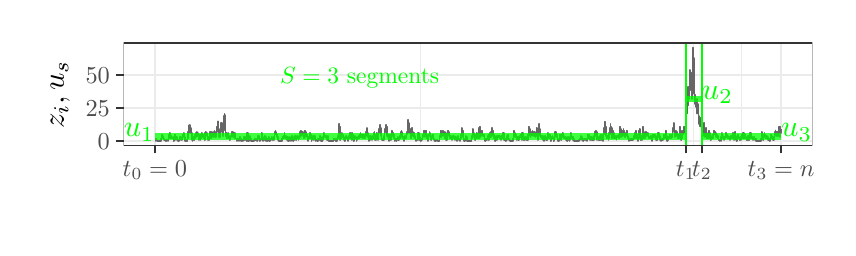
\begin{tikzpicture}[x=1pt,y=1pt]
\definecolor{fillColor}{RGB}{255,255,255}
\path[use as bounding box,fill=fillColor,fill opacity=0.00] (0,0) rectangle (289.08, 72.27);
\begin{scope}
\path[clip] (  0.00,  0.00) rectangle (289.08, 72.27);
\definecolor{drawColor}{RGB}{255,255,255}
\definecolor{fillColor}{RGB}{255,255,255}

\path[draw=drawColor,line width= 0.6pt,line join=round,line cap=round,fill=fillColor] (  0.00,  0.00) rectangle (289.08, 72.27);
\end{scope}
\begin{scope}
\path[clip] ( 34.65, 29.59) rectangle (283.58, 66.77);
\definecolor{fillColor}{RGB}{255,255,255}

\path[fill=fillColor] ( 34.65, 29.59) rectangle (283.58, 66.77);
\definecolor{drawColor}{gray}{0.92}

\path[draw=drawColor,line width= 0.3pt,line join=round] (141.89, 29.59) --
	(141.89, 66.77);

\path[draw=drawColor,line width= 0.3pt,line join=round] (240.71, 29.59) --
	(240.71, 66.77);

\path[draw=drawColor,line width= 0.3pt,line join=round] (257.94, 29.59) --
	(257.94, 66.77);

\path[draw=drawColor,line width= 0.6pt,line join=round] ( 34.65, 31.28) --
	(283.58, 31.28);

\path[draw=drawColor,line width= 0.6pt,line join=round] ( 34.65, 43.18) --
	(283.58, 43.18);

\path[draw=drawColor,line width= 0.6pt,line join=round] ( 34.65, 55.08) --
	(283.58, 55.08);

\path[draw=drawColor,line width= 0.6pt,line join=round] ( 45.97, 29.59) --
	( 45.97, 66.77);

\path[draw=drawColor,line width= 0.6pt,line join=round] (237.82, 29.59) --
	(237.82, 66.77);

\path[draw=drawColor,line width= 0.6pt,line join=round] (243.61, 29.59) --
	(243.61, 66.77);

\path[draw=drawColor,line width= 0.6pt,line join=round] (272.26, 29.59) --
	(272.26, 66.77);
\definecolor{drawColor}{gray}{0.40}

\path[draw=drawColor,line width= 0.6pt,line join=round] ( 45.97, 31.75) --
	( 46.15, 31.75) --
	( 46.15, 31.28) --
	( 46.17, 31.28) --
	( 46.17, 31.75) --
	( 46.18, 31.75) --
	( 46.18, 32.23) --
	( 46.60, 32.23) --
	( 46.60, 31.75) --
	( 46.63, 31.75) --
	( 46.63, 31.28) --
	( 48.22, 31.28) --
	( 48.22, 31.75) --
	( 48.26, 31.75) --
	( 48.26, 32.23) --
	( 48.49, 32.23) --
	( 48.49, 32.71) --
	( 48.56, 32.71) --
	( 48.56, 33.18) --
	( 48.63, 33.18) --
	( 48.63, 33.66) --
	( 48.67, 33.66) --
	( 48.67, 33.18) --
	( 48.71, 33.18) --
	( 48.71, 32.71) --
	( 48.83, 32.71) --
	( 48.83, 33.18) --
	( 48.94, 33.18) --
	( 48.94, 32.71) --
	( 49.00, 32.71) --
	( 49.00, 33.18) --
	( 49.01, 33.18) --
	( 49.01, 32.71) --
	( 49.08, 32.71) --
	( 49.08, 32.23) --
	( 49.29, 32.23) --
	( 49.29, 31.75) --
	( 49.31, 31.75) --
	( 49.31, 32.23) --
	( 49.45, 32.23) --
	( 49.45, 31.75) --
	( 49.76, 31.75) --
	( 49.76, 31.28) --
	( 50.20, 31.28) --
	( 50.20, 31.75) --
	( 50.65, 31.75) --
	( 50.65, 31.28) --
	( 50.68, 31.28) --
	( 50.68, 31.75) --
	( 50.86, 31.75) --
	( 50.86, 32.23) --
	( 50.96, 32.23) --
	( 50.96, 32.71) --
	( 51.04, 32.71) --
	( 51.04, 33.18) --
	( 51.06, 33.18) --
	( 51.06, 33.66) --
	( 51.14, 33.66) --
	( 51.14, 33.18) --
	( 51.20, 33.18) --
	( 51.20, 33.66) --
	( 51.30, 33.66) --
	( 51.30, 34.13) --
	( 51.31, 34.13) --
	( 51.31, 33.66) --
	( 51.32, 33.66) --
	( 51.32, 34.13) --
	( 51.41, 34.13) --
	( 51.41, 33.66) --
	( 51.47, 33.66) --
	( 51.47, 34.13) --
	( 51.50, 34.13) --
	( 51.50, 33.66) --
	( 51.51, 33.66) --
	( 51.51, 33.18) --
	( 51.53, 33.18) --
	( 51.53, 33.66) --
	( 51.65, 33.66) --
	( 51.65, 33.18) --
	( 51.75, 33.18) --
	( 51.75, 32.71) --
	( 51.77, 32.71) --
	( 51.77, 32.23) --
	( 51.80, 32.23) --
	( 51.80, 32.71) --
	( 51.82, 32.71) --
	( 51.82, 33.18) --
	( 51.93, 33.18) --
	( 51.93, 32.71) --
	( 51.97, 32.71) --
	( 51.97, 32.23) --
	( 52.26, 32.23) --
	( 52.26, 32.71) --
	( 52.27, 32.71) --
	( 52.27, 32.23) --
	( 52.70, 32.23) --
	( 52.70, 31.28) --
	( 52.81, 31.28) --
	( 52.81, 31.75) --
	( 52.83, 31.75) --
	( 52.83, 32.23) --
	( 52.88, 32.23) --
	( 52.88, 32.71) --
	( 53.02, 32.71) --
	( 53.02, 33.18) --
	( 53.10, 33.18) --
	( 53.10, 33.66) --
	( 53.26, 33.66) --
	( 53.26, 33.18) --
	( 53.29, 33.18) --
	( 53.29, 32.71) --
	( 53.34, 32.71) --
	( 53.34, 32.23) --
	( 53.34, 32.23) --
	( 53.34, 32.71) --
	( 53.47, 32.71) --
	( 53.47, 32.23) --
	( 53.55, 32.23) --
	( 53.55, 31.75) --
	( 53.60, 31.75) --
	( 53.60, 32.23) --
	( 53.69, 32.23) --
	( 53.69, 32.71) --
	( 53.79, 32.71) --
	( 53.79, 32.23) --
	( 53.98, 32.23) --
	( 53.98, 32.71) --
	( 54.05, 32.71) --
	( 54.05, 32.23) --
	( 54.14, 32.23) --
	( 54.14, 31.75) --
	( 54.43, 31.75) --
	( 54.43, 31.28) --
	( 54.79, 31.28) --
	( 54.79, 31.75) --
	( 55.03, 31.75) --
	( 55.03, 32.23) --
	( 55.09, 32.23) --
	( 55.09, 32.71) --
	( 55.25, 32.71) --
	( 55.25, 32.23) --
	( 55.35, 32.23) --
	( 55.35, 32.71) --
	( 55.48, 32.71) --
	( 55.48, 32.23) --
	( 55.54, 32.23) --
	( 55.54, 31.75) --
	( 55.78, 31.75) --
	( 55.78, 32.23) --
	( 55.80, 32.23) --
	( 55.80, 31.75) --
	( 55.81, 31.75) --
	( 55.81, 32.23) --
	( 55.98, 32.23) --
	( 55.98, 33.18) --
	( 56.17, 33.18) --
	( 56.17, 33.66) --
	( 56.23, 33.66) --
	( 56.23, 33.18) --
	( 56.27, 33.18) --
	( 56.27, 32.71) --
	( 56.41, 32.71) --
	( 56.41, 33.66) --
	( 56.43, 33.66) --
	( 56.43, 34.13) --
	( 56.44, 34.13) --
	( 56.44, 33.18) --
	( 56.62, 33.18) --
	( 56.62, 32.71) --
	( 56.87, 32.71) --
	( 56.87, 31.75) --
	( 56.87, 31.75) --
	( 56.87, 31.28) --
	( 57.13, 31.28) --
	( 57.13, 31.75) --
	( 57.59, 31.75) --
	( 57.59, 31.28) --
	( 57.72, 31.28) --
	( 57.72, 31.75) --
	( 57.77, 31.75) --
	( 57.77, 32.23) --
	( 57.82, 32.23) --
	( 57.82, 33.18) --
	( 57.91, 33.18) --
	( 57.91, 34.13) --
	( 58.05, 34.13) --
	( 58.05, 34.61) --
	( 58.10, 34.61) --
	( 58.10, 35.09) --
	( 58.17, 35.09) --
	( 58.17, 34.61) --
	( 58.20, 34.61) --
	( 58.20, 36.04) --
	( 58.22, 36.04) --
	( 58.22, 36.51) --
	( 58.22, 36.51) --
	( 58.22, 36.04) --
	( 58.27, 36.04) --
	( 58.27, 36.99) --
	( 58.27, 36.99) --
	( 58.27, 36.04) --
	( 58.34, 36.04) --
	( 58.34, 36.51) --
	( 58.37, 36.51) --
	( 58.37, 35.56) --
	( 58.43, 35.56) --
	( 58.43, 36.04) --
	( 58.51, 36.04) --
	( 58.51, 35.56) --
	( 58.56, 35.56) --
	( 58.56, 35.09) --
	( 58.59, 35.09) --
	( 58.59, 36.51) --
	( 58.64, 36.51) --
	( 58.64, 36.99) --
	( 58.65, 36.99) --
	( 58.65, 36.51) --
	( 58.65, 36.51) --
	( 58.65, 35.56) --
	( 58.67, 35.56) --
	( 58.67, 35.09) --
	( 58.73, 35.09) --
	( 58.73, 34.13) --
	( 58.81, 34.13) --
	( 58.81, 34.61) --
	( 58.84, 34.61) --
	( 58.84, 35.09) --
	( 58.84, 35.09) --
	( 58.84, 35.56) --
	( 58.89, 35.56) --
	( 58.89, 35.09) --
	( 58.99, 35.09) --
	( 58.99, 35.56) --
	( 59.02, 35.56) --
	( 59.02, 36.04) --
	( 59.04, 36.04) --
	( 59.04, 34.61) --
	( 59.05, 34.61) --
	( 59.05, 35.09) --
	( 59.09, 35.09) --
	( 59.09, 34.61) --
	( 59.25, 34.61) --
	( 59.25, 34.13) --
	( 59.27, 34.13) --
	( 59.27, 33.66) --
	( 59.29, 33.66) --
	( 59.29, 32.71) --
	( 59.45, 32.71) --
	( 59.45, 31.75) --
	( 59.51, 31.75) --
	( 59.51, 31.28) --
	( 59.56, 31.28) --
	( 59.56, 31.75) --
	( 59.65, 31.75) --
	( 59.65, 32.23) --
	( 59.87, 32.23) --
	( 59.87, 32.71) --
	( 60.00, 32.71) --
	( 60.00, 32.23) --
	( 60.10, 32.23) --
	( 60.10, 31.75) --
	( 60.22, 31.75) --
	( 60.22, 32.23) --
	( 60.32, 32.23) --
	( 60.32, 31.75) --
	( 60.33, 31.75) --
	( 60.33, 32.23) --
	( 60.37, 32.23) --
	( 60.37, 32.71) --
	( 60.39, 32.71) --
	( 60.39, 33.18) --
	( 60.56, 33.18) --
	( 60.56, 33.66) --
	( 60.67, 33.66) --
	( 60.67, 33.18) --
	( 60.69, 33.18) --
	( 60.69, 33.66) --
	( 60.78, 33.66) --
	( 60.78, 33.18) --
	( 60.82, 33.18) --
	( 60.82, 32.71) --
	( 60.83, 32.71) --
	( 60.83, 33.66) --
	( 60.85, 33.66) --
	( 60.85, 33.18) --
	( 60.92, 33.18) --
	( 60.92, 33.66) --
	( 60.94, 33.66) --
	( 60.94, 34.13) --
	( 61.09, 34.13) --
	( 61.09, 34.61) --
	( 61.14, 34.61) --
	( 61.14, 34.13) --
	( 61.23, 34.13) --
	( 61.23, 34.61) --
	( 61.28, 34.61) --
	( 61.28, 33.66) --
	( 61.37, 33.66) --
	( 61.37, 34.13) --
	( 61.38, 34.13) --
	( 61.38, 33.66) --
	( 61.39, 33.66) --
	( 61.39, 33.18) --
	( 61.42, 33.18) --
	( 61.42, 34.13) --
	( 61.46, 34.13) --
	( 61.46, 33.66) --
	( 61.54, 33.66) --
	( 61.54, 33.18) --
	( 61.68, 33.18) --
	( 61.68, 32.71) --
	( 61.79, 32.71) --
	( 61.79, 33.18) --
	( 61.82, 33.18) --
	( 61.82, 32.71) --
	( 61.88, 32.71) --
	( 61.88, 31.75) --
	( 61.89, 31.75) --
	( 61.89, 32.23) --
	( 61.91, 32.23) --
	( 61.91, 32.71) --
	( 61.96, 32.71) --
	( 61.96, 33.18) --
	( 62.22, 33.18) --
	( 62.22, 33.66) --
	( 62.23, 33.66) --
	( 62.23, 33.18) --
	( 62.34, 33.18) --
	( 62.34, 32.71) --
	( 62.36, 32.71) --
	( 62.36, 32.23) --
	( 62.42, 32.23) --
	( 62.42, 31.75) --
	( 62.50, 31.75) --
	( 62.50, 32.23) --
	( 62.61, 32.23) --
	( 62.61, 32.71) --
	( 62.63, 32.71) --
	( 62.63, 33.18) --
	( 62.64, 33.18) --
	( 62.64, 33.66) --
	( 62.66, 33.66) --
	( 62.66, 33.18) --
	( 62.68, 33.18) --
	( 62.68, 33.66) --
	( 62.75, 33.66) --
	( 62.75, 34.13) --
	( 62.95, 34.13) --
	( 62.95, 33.66) --
	( 63.03, 33.66) --
	( 63.03, 34.13) --
	( 63.09, 34.13) --
	( 63.09, 33.66) --
	( 63.09, 33.66) --
	( 63.09, 33.18) --
	( 63.10, 33.18) --
	( 63.10, 33.66) --
	( 63.14, 33.66) --
	( 63.14, 33.18) --
	( 63.20, 33.18) --
	( 63.20, 32.71) --
	( 63.42, 32.71) --
	( 63.42, 33.18) --
	( 63.45, 33.18) --
	( 63.45, 33.66) --
	( 63.48, 33.66) --
	( 63.48, 33.18) --
	( 63.51, 33.18) --
	( 63.51, 32.71) --
	( 63.55, 32.71) --
	( 63.55, 32.23) --
	( 63.86, 32.23) --
	( 63.86, 32.71) --
	( 63.87, 32.71) --
	( 63.87, 32.23) --
	( 63.91, 32.23) --
	( 63.91, 31.75) --
	( 63.96, 31.75) --
	( 63.96, 32.23) --
	( 63.97, 32.23) --
	( 63.97, 32.71) --
	( 64.06, 32.71) --
	( 64.06, 33.18) --
	( 64.14, 33.18) --
	( 64.14, 33.66) --
	( 64.17, 33.66) --
	( 64.17, 34.13) --
	( 64.25, 34.13) --
	( 64.25, 34.61) --
	( 64.31, 34.61) --
	( 64.31, 34.13) --
	( 64.39, 34.13) --
	( 64.39, 34.61) --
	( 64.41, 34.61) --
	( 64.41, 34.13) --
	( 64.42, 34.13) --
	( 64.42, 33.66) --
	( 64.48, 33.66) --
	( 64.48, 33.18) --
	( 64.52, 33.18) --
	( 64.52, 33.66) --
	( 64.58, 33.66) --
	( 64.58, 34.13) --
	( 64.59, 34.13) --
	( 64.59, 33.66) --
	( 64.60, 33.66) --
	( 64.60, 34.13) --
	( 64.62, 34.13) --
	( 64.62, 33.66) --
	( 64.65, 33.66) --
	( 64.65, 34.13) --
	( 64.71, 34.13) --
	( 64.71, 33.66) --
	( 64.76, 33.66) --
	( 64.76, 34.13) --
	( 64.85, 34.13) --
	( 64.85, 33.66) --
	( 64.97, 33.66) --
	( 64.97, 33.18) --
	( 65.04, 33.18) --
	( 65.04, 32.71) --
	( 65.05, 32.71) --
	( 65.05, 32.23) --
	( 65.10, 32.23) --
	( 65.10, 31.75) --
	( 65.13, 31.75) --
	( 65.13, 32.23) --
	( 65.15, 32.23) --
	( 65.15, 31.75) --
	( 65.28, 31.75) --
	( 65.28, 32.23) --
	( 65.53, 32.23) --
	( 65.53, 32.71) --
	( 65.58, 32.71) --
	( 65.58, 32.23) --
	( 65.73, 32.23) --
	( 65.73, 31.75) --
	( 65.76, 31.75) --
	( 65.76, 32.71) --
	( 65.78, 32.71) --
	( 65.78, 33.18) --
	( 65.80, 33.18) --
	( 65.80, 33.66) --
	( 65.82, 33.66) --
	( 65.82, 34.13) --
	( 65.86, 34.13) --
	( 65.86, 34.61) --
	( 65.98, 34.61) --
	( 65.98, 34.13) --
	( 66.05, 34.13) --
	( 66.05, 34.61) --
	( 66.21, 34.61) --
	( 66.21, 33.66) --
	( 66.24, 33.66) --
	( 66.24, 33.18) --
	( 66.24, 33.18) --
	( 66.24, 32.71) --
	( 66.31, 32.71) --
	( 66.31, 32.23) --
	( 66.39, 32.23) --
	( 66.39, 32.71) --
	( 66.41, 32.71) --
	( 66.41, 33.66) --
	( 66.53, 33.66) --
	( 66.53, 34.13) --
	( 66.58, 34.13) --
	( 66.58, 34.61) --
	( 66.72, 34.61) --
	( 66.72, 34.13) --
	( 66.84, 34.13) --
	( 66.84, 33.66) --
	( 66.86, 33.66) --
	( 66.86, 32.71) --
	( 66.89, 32.71) --
	( 66.89, 33.18) --
	( 66.96, 33.18) --
	( 66.96, 32.71) --
	( 66.98, 32.71) --
	( 66.98, 33.18) --
	( 66.99, 33.18) --
	( 66.99, 32.71) --
	( 67.02, 32.71) --
	( 67.02, 33.18) --
	( 67.03, 33.18) --
	( 67.03, 32.71) --
	( 67.09, 32.71) --
	( 67.09, 33.18) --
	( 67.16, 33.18) --
	( 67.16, 33.66) --
	( 67.19, 33.66) --
	( 67.19, 34.13) --
	( 67.27, 34.13) --
	( 67.27, 34.61) --
	( 67.34, 34.61) --
	( 67.34, 34.13) --
	( 67.34, 34.13) --
	( 67.34, 34.61) --
	( 67.43, 34.61) --
	( 67.43, 34.13) --
	( 67.46, 34.13) --
	( 67.46, 34.61) --
	( 67.47, 34.61) --
	( 67.47, 35.09) --
	( 67.48, 35.09) --
	( 67.48, 34.61) --
	( 67.54, 34.61) --
	( 67.54, 34.13) --
	( 67.62, 34.13) --
	( 67.62, 33.66) --
	( 67.64, 33.66) --
	( 67.64, 33.18) --
	( 67.72, 33.18) --
	( 67.72, 32.71) --
	( 67.73, 32.71) --
	( 67.73, 33.18) --
	( 67.76, 33.18) --
	( 67.76, 34.13) --
	( 67.80, 34.13) --
	( 67.80, 33.66) --
	( 67.91, 33.66) --
	( 67.91, 33.18) --
	( 67.92, 33.18) --
	( 67.92, 32.71) --
	( 67.94, 32.71) --
	( 67.94, 33.18) --
	( 67.99, 33.18) --
	( 67.99, 33.66) --
	( 68.06, 33.66) --
	( 68.06, 34.13) --
	( 68.16, 34.13) --
	( 68.16, 34.61) --
	( 68.18, 34.61) --
	( 68.18, 34.13) --
	( 68.20, 34.13) --
	( 68.20, 34.61) --
	( 68.20, 34.61) --
	( 68.20, 35.09) --
	( 68.21, 35.09) --
	( 68.21, 34.61) --
	( 68.21, 34.61) --
	( 68.21, 34.13) --
	( 68.24, 34.13) --
	( 68.24, 34.61) --
	( 68.39, 34.61) --
	( 68.39, 35.09) --
	( 68.39, 35.09) --
	( 68.39, 34.61) --
	( 68.44, 34.61) --
	( 68.44, 35.09) --
	( 68.44, 35.09) --
	( 68.44, 34.61) --
	( 68.46, 34.61) --
	( 68.46, 36.04) --
	( 68.47, 36.04) --
	( 68.47, 36.51) --
	( 68.49, 36.51) --
	( 68.49, 36.04) --
	( 68.51, 36.04) --
	( 68.51, 36.51) --
	( 68.56, 36.51) --
	( 68.56, 36.99) --
	( 68.60, 36.99) --
	( 68.60, 37.47) --
	( 68.61, 37.47) --
	( 68.61, 36.99) --
	( 68.65, 36.99) --
	( 68.65, 36.51) --
	( 68.66, 36.51) --
	( 68.66, 36.04) --
	( 68.66, 36.04) --
	( 68.66, 36.51) --
	( 68.69, 36.51) --
	( 68.69, 36.99) --
	( 68.69, 36.99) --
	( 68.69, 36.51) --
	( 68.70, 36.51) --
	( 68.70, 37.47) --
	( 68.77, 37.47) --
	( 68.77, 37.94) --
	( 68.83, 37.94) --
	( 68.83, 38.42) --
	( 68.83, 38.42) --
	( 68.83, 37.94) --
	( 68.89, 37.94) --
	( 68.89, 37.47) --
	( 68.92, 37.47) --
	( 68.92, 36.04) --
	( 68.92, 36.04) --
	( 68.92, 35.09) --
	( 68.93, 35.09) --
	( 68.93, 35.56) --
	( 68.99, 35.56) --
	( 68.99, 36.04) --
	( 69.01, 36.04) --
	( 69.01, 35.56) --
	( 69.05, 35.56) --
	( 69.05, 35.09) --
	( 69.06, 35.09) --
	( 69.06, 34.61) --
	( 69.14, 34.61) --
	( 69.14, 34.13) --
	( 69.16, 34.13) --
	( 69.16, 33.18) --
	( 69.20, 33.18) --
	( 69.20, 33.66) --
	( 69.21, 33.66) --
	( 69.21, 32.71) --
	( 69.30, 32.71) --
	( 69.30, 33.18) --
	( 69.38, 33.18) --
	( 69.38, 33.66) --
	( 69.39, 33.66) --
	( 69.39, 33.18) --
	( 69.44, 33.18) --
	( 69.44, 32.71) --
	( 69.51, 32.71) --
	( 69.51, 33.66) --
	( 69.55, 33.66) --
	( 69.55, 34.13) --
	( 69.59, 34.13) --
	( 69.59, 34.61) --
	( 69.59, 34.61) --
	( 69.59, 34.13) --
	( 69.66, 34.13) --
	( 69.66, 34.61) --
	( 69.68, 34.61) --
	( 69.68, 35.09) --
	( 69.75, 35.09) --
	( 69.75, 34.61) --
	( 69.78, 34.61) --
	( 69.78, 35.09) --
	( 69.79, 35.09) --
	( 69.79, 35.56) --
	( 69.82, 35.56) --
	( 69.82, 36.04) --
	( 69.85, 36.04) --
	( 69.85, 35.56) --
	( 69.87, 35.56) --
	( 69.87, 36.04) --
	( 69.90, 36.04) --
	( 69.90, 36.51) --
	( 69.92, 36.51) --
	( 69.92, 36.99) --
	( 69.92, 36.99) --
	( 69.92, 37.47) --
	( 69.97, 37.47) --
	( 69.97, 37.94) --
	( 70.00, 37.94) --
	( 70.00, 37.47) --
	( 70.02, 37.47) --
	( 70.02, 37.94) --
	( 70.04, 37.94) --
	( 70.04, 37.47) --
	( 70.05, 37.47) --
	( 70.05, 36.99) --
	( 70.08, 36.99) --
	( 70.08, 37.47) --
	( 70.09, 37.47) --
	( 70.09, 37.94) --
	( 70.11, 37.94) --
	( 70.11, 37.47) --
	( 70.19, 37.47) --
	( 70.19, 37.94) --
	( 70.24, 37.94) --
	( 70.24, 37.47) --
	( 70.27, 37.47) --
	( 70.27, 36.99) --
	( 70.28, 36.99) --
	( 70.28, 37.47) --
	( 70.29, 37.47) --
	( 70.29, 36.99) --
	( 70.32, 36.99) --
	( 70.32, 37.47) --
	( 70.35, 37.47) --
	( 70.35, 36.99) --
	( 70.37, 36.99) --
	( 70.37, 36.51) --
	( 70.38, 36.51) --
	( 70.38, 36.04) --
	( 70.41, 36.04) --
	( 70.41, 35.56) --
	( 70.43, 35.56) --
	( 70.43, 35.09) --
	( 70.47, 35.09) --
	( 70.47, 34.61) --
	( 70.52, 34.61) --
	( 70.52, 34.13) --
	( 70.53, 34.13) --
	( 70.53, 34.61) --
	( 70.54, 34.61) --
	( 70.54, 34.13) --
	( 70.54, 34.13) --
	( 70.54, 33.66) --
	( 70.59, 33.66) --
	( 70.59, 33.18) --
	( 70.60, 33.18) --
	( 70.60, 33.66) --
	( 70.63, 33.66) --
	( 70.63, 34.13) --
	( 70.64, 34.13) --
	( 70.64, 33.66) --
	( 70.72, 33.66) --
	( 70.72, 34.13) --
	( 70.73, 34.13) --
	( 70.73, 33.66) --
	( 70.77, 33.66) --
	( 70.77, 33.18) --
	( 70.79, 33.18) --
	( 70.79, 33.66) --
	( 70.79, 33.66) --
	( 70.79, 34.61) --
	( 70.80, 34.61) --
	( 70.80, 35.09) --
	( 70.86, 35.09) --
	( 70.86, 35.56) --
	( 70.89, 35.56) --
	( 70.89, 36.04) --
	( 70.91, 36.04) --
	( 70.91, 36.51) --
	( 70.91, 36.51) --
	( 70.91, 36.99) --
	( 70.95, 36.99) --
	( 70.95, 37.47) --
	( 70.97, 37.47) --
	( 70.97, 37.94) --
	( 70.98, 37.94) --
	( 70.98, 37.47) --
	( 70.98, 37.47) --
	( 70.98, 37.94) --
	( 71.00, 37.94) --
	( 71.00, 39.37) --
	( 71.02, 39.37) --
	( 71.02, 39.85) --
	( 71.04, 39.85) --
	( 71.04, 39.37) --
	( 71.05, 39.37) --
	( 71.05, 39.85) --
	( 71.06, 39.85) --
	( 71.06, 40.32) --
	( 71.07, 40.32) --
	( 71.07, 40.80) --
	( 71.08, 40.80) --
	( 71.08, 41.27) --
	( 71.09, 41.27) --
	( 71.09, 40.80) --
	( 71.14, 40.80) --
	( 71.14, 41.27) --
	( 71.17, 41.27) --
	( 71.17, 40.80) --
	( 71.24, 40.80) --
	( 71.24, 40.32) --
	( 71.25, 40.32) --
	( 71.25, 39.85) --
	( 71.26, 39.85) --
	( 71.26, 39.37) --
	( 71.31, 39.37) --
	( 71.31, 38.89) --
	( 71.35, 38.89) --
	( 71.35, 38.42) --
	( 71.36, 38.42) --
	( 71.36, 37.94) --
	( 71.36, 37.94) --
	( 71.36, 37.47) --
	( 71.40, 37.47) --
	( 71.40, 36.99) --
	( 71.42, 36.99) --
	( 71.42, 36.51) --
	( 71.44, 36.51) --
	( 71.44, 36.04) --
	( 71.45, 36.04) --
	( 71.45, 34.61) --
	( 71.46, 34.61) --
	( 71.46, 35.09) --
	( 71.47, 35.09) --
	( 71.47, 34.13) --
	( 71.50, 34.13) --
	( 71.50, 33.66) --
	( 71.51, 33.66) --
	( 71.51, 33.18) --
	( 71.52, 33.18) --
	( 71.52, 33.66) --
	( 71.53, 33.66) --
	( 71.53, 34.13) --
	( 71.54, 34.13) --
	( 71.54, 33.66) --
	( 71.59, 33.66) --
	( 71.59, 33.18) --
	( 71.71, 33.18) --
	( 71.71, 34.13) --
	( 71.91, 34.13) --
	( 71.91, 33.66) --
	( 71.97, 33.66) --
	( 71.97, 32.23) --
	( 72.14, 32.23) --
	( 72.14, 33.18) --
	( 72.16, 33.18) --
	( 72.16, 32.23) --
	( 72.25, 32.23) --
	( 72.25, 32.71) --
	( 72.38, 32.71) --
	( 72.38, 33.18) --
	( 72.52, 33.18) --
	( 72.52, 33.66) --
	( 72.53, 33.66) --
	( 72.53, 34.13) --
	( 72.59, 34.13) --
	( 72.59, 33.18) --
	( 72.69, 33.18) --
	( 72.69, 32.71) --
	( 72.83, 32.71) --
	( 72.83, 32.23) --
	( 72.84, 32.23) --
	( 72.84, 32.71) --
	( 72.97, 32.71) --
	( 72.97, 32.23) --
	( 72.98, 32.23) --
	( 72.98, 31.75) --
	( 73.00, 31.75) --
	( 73.00, 32.23) --
	( 73.01, 32.23) --
	( 73.01, 32.71) --
	( 73.28, 32.71) --
	( 73.28, 33.18) --
	( 73.29, 33.18) --
	( 73.29, 32.71) --
	( 73.43, 32.71) --
	( 73.43, 33.18) --
	( 73.46, 33.18) --
	( 73.46, 32.71) --
	( 73.53, 32.71) --
	( 73.53, 33.18) --
	( 73.66, 33.18) --
	( 73.66, 33.66) --
	( 73.73, 33.66) --
	( 73.73, 33.18) --
	( 73.77, 33.18) --
	( 73.77, 33.66) --
	( 73.83, 33.66) --
	( 73.83, 34.61) --
	( 73.88, 34.61) --
	( 73.88, 34.13) --
	( 73.91, 34.13) --
	( 73.91, 33.66) --
	( 73.98, 33.66) --
	( 73.98, 33.18) --
	( 74.03, 33.18) --
	( 74.03, 33.66) --
	( 74.05, 33.66) --
	( 74.05, 34.13) --
	( 74.11, 34.13) --
	( 74.11, 33.66) --
	( 74.16, 33.66) --
	( 74.16, 34.13) --
	( 74.20, 34.13) --
	( 74.20, 34.61) --
	( 74.21, 34.61) --
	( 74.21, 34.13) --
	( 74.21, 34.13) --
	( 74.21, 33.66) --
	( 74.24, 33.66) --
	( 74.24, 33.18) --
	( 74.28, 33.18) --
	( 74.28, 32.71) --
	( 74.36, 32.71) --
	( 74.36, 33.18) --
	( 74.38, 33.18) --
	( 74.38, 33.66) --
	( 74.41, 33.66) --
	( 74.41, 33.18) --
	( 74.50, 33.18) --
	( 74.50, 32.71) --
	( 74.52, 32.71) --
	( 74.52, 33.18) --
	( 74.52, 33.18) --
	( 74.52, 33.66) --
	( 74.62, 33.66) --
	( 74.62, 34.13) --
	( 74.65, 34.13) --
	( 74.65, 33.66) --
	( 74.65, 33.66) --
	( 74.65, 34.13) --
	( 74.81, 34.13) --
	( 74.81, 33.66) --
	( 74.83, 33.66) --
	( 74.83, 33.18) --
	( 74.97, 33.18) --
	( 74.97, 32.23) --
	( 75.05, 32.23) --
	( 75.05, 32.71) --
	( 75.07, 32.71) --
	( 75.07, 32.23) --
	( 75.08, 32.23) --
	( 75.08, 32.71) --
	( 75.10, 32.71) --
	( 75.10, 32.23) --
	( 75.50, 32.23) --
	( 75.50, 31.75) --
	( 75.53, 31.75) --
	( 75.53, 31.28) --
	( 75.72, 31.28) --
	( 75.72, 31.75) --
	( 75.83, 31.75) --
	( 75.83, 32.23) --
	( 76.12, 32.23) --
	( 76.12, 31.75) --
	( 76.28, 31.75) --
	( 76.28, 31.28) --
	( 76.47, 31.28) --
	( 76.47, 31.75) --
	( 76.53, 31.75) --
	( 76.53, 32.23) --
	( 76.54, 32.23) --
	( 76.54, 32.71) --
	( 76.92, 32.71) --
	( 76.92, 32.23) --
	( 76.98, 32.23) --
	( 76.98, 31.75) --
	( 76.99, 31.75) --
	( 76.99, 31.28) --
	( 77.22, 31.28) --
	( 77.22, 31.75) --
	( 77.68, 31.75) --
	( 77.68, 31.28) --
	( 77.89, 31.28) --
	( 77.89, 31.75) --
	( 78.03, 31.75) --
	( 78.03, 32.23) --
	( 78.20, 32.23) --
	( 78.20, 32.71) --
	( 78.24, 32.71) --
	( 78.24, 32.23) --
	( 78.35, 32.23) --
	( 78.35, 31.75) --
	( 78.51, 31.75) --
	( 78.51, 32.23) --
	( 78.57, 32.23) --
	( 78.57, 32.71) --
	( 78.65, 32.71) --
	( 78.65, 32.23) --
	( 78.96, 32.23) --
	( 78.96, 31.75) --
	( 79.02, 31.75) --
	( 79.02, 31.28) --
	( 79.20, 31.28) --
	( 79.20, 32.71) --
	( 79.23, 32.71) --
	( 79.23, 34.13) --
	( 79.65, 34.13) --
	( 79.65, 32.71) --
	( 79.68, 32.71) --
	( 79.68, 32.23) --
	( 79.68, 32.23) --
	( 79.68, 31.28) --
	( 79.93, 31.28) --
	( 79.93, 31.75) --
	( 79.96, 31.75) --
	( 79.96, 32.23) --
	( 80.14, 32.23) --
	( 80.14, 32.71) --
	( 80.29, 32.71) --
	( 80.29, 33.18) --
	( 80.35, 33.18) --
	( 80.35, 32.71) --
	( 80.41, 32.71) --
	( 80.41, 32.23) --
	( 80.59, 32.23) --
	( 80.59, 31.75) --
	( 80.74, 31.75) --
	( 80.74, 31.28) --
	( 81.79, 31.28) --
	( 81.79, 31.75) --
	( 82.03, 31.75) --
	( 82.03, 32.23) --
	( 82.24, 32.23) --
	( 82.24, 31.75) --
	( 82.27, 31.75) --
	( 82.27, 32.23) --
	( 82.48, 32.23) --
	( 82.48, 31.75) --
	( 82.53, 31.75) --
	( 82.53, 32.23) --
	( 82.72, 32.23) --
	( 82.72, 31.75) --
	( 82.98, 31.75) --
	( 82.98, 31.28) --
	( 83.02, 31.28) --
	( 83.02, 31.75) --
	( 83.25, 31.75) --
	( 83.25, 32.23) --
	( 83.28, 32.23) --
	( 83.28, 32.71) --
	( 83.29, 32.71) --
	( 83.29, 33.18) --
	( 83.47, 33.18) --
	( 83.47, 32.71) --
	( 83.71, 32.71) --
	( 83.71, 32.23) --
	( 83.73, 32.23) --
	( 83.73, 31.75) --
	( 83.74, 31.75) --
	( 83.74, 31.28) --
	( 83.85, 31.28) --
	( 83.85, 31.75) --
	( 84.23, 31.75) --
	( 84.23, 32.23) --
	( 84.30, 32.23) --
	( 84.30, 31.75) --
	( 84.38, 31.75) --
	( 84.38, 32.23) --
	( 84.46, 32.23) --
	( 84.46, 32.71) --
	( 84.49, 32.71) --
	( 84.49, 33.66) --
	( 84.51, 33.66) --
	( 84.51, 34.13) --
	( 84.68, 34.13) --
	( 84.68, 33.66) --
	( 84.83, 33.66) --
	( 84.83, 33.18) --
	( 84.91, 33.18) --
	( 84.91, 32.71) --
	( 84.95, 32.71) --
	( 84.95, 31.75) --
	( 84.96, 31.75) --
	( 84.96, 31.28) --
	( 84.99, 31.28) --
	( 84.99, 31.75) --
	( 85.22, 31.75) --
	( 85.22, 32.23) --
	( 85.44, 32.23) --
	( 85.44, 31.75) --
	( 85.57, 31.75) --
	( 85.57, 32.23) --
	( 85.63, 32.23) --
	( 85.63, 33.18) --
	( 85.67, 33.18) --
	( 85.67, 32.71) --
	( 86.02, 32.71) --
	( 86.02, 32.23) --
	( 86.08, 32.23) --
	( 86.08, 31.28) --
	( 86.14, 31.28) --
	( 86.14, 31.75) --
	( 86.38, 31.75) --
	( 86.38, 32.23) --
	( 86.59, 32.23) --
	( 86.59, 31.28) --
	( 86.66, 31.28) --
	( 86.66, 31.75) --
	( 86.80, 31.75) --
	( 86.80, 32.23) --
	( 87.05, 32.23) --
	( 87.05, 32.71) --
	( 87.09, 32.71) --
	( 87.09, 32.23) --
	( 87.24, 32.23) --
	( 87.24, 31.28) --
	( 87.50, 31.28) --
	( 87.50, 31.75) --
	( 87.93, 31.75) --
	( 87.93, 32.23) --
	( 87.95, 32.23) --
	( 87.95, 31.75) --
	( 88.03, 31.75) --
	( 88.03, 32.23) --
	( 88.20, 32.23) --
	( 88.20, 32.71) --
	( 88.38, 32.71) --
	( 88.38, 32.23) --
	( 88.49, 32.23) --
	( 88.49, 31.75) --
	( 88.50, 31.75) --
	( 88.50, 32.23) --
	( 88.63, 32.23) --
	( 88.63, 31.75) --
	( 88.76, 31.75) --
	( 88.76, 32.23) --
	( 88.95, 32.23) --
	( 88.95, 31.75) --
	( 89.11, 31.75) --
	( 89.11, 32.23) --
	( 89.12, 32.23) --
	( 89.12, 32.71) --
	( 89.17, 32.71) --
	( 89.17, 33.66) --
	( 89.21, 33.66) --
	( 89.21, 33.18) --
	( 89.25, 33.18) --
	( 89.25, 33.66) --
	( 89.28, 33.66) --
	( 89.28, 34.13) --
	( 89.39, 34.13) --
	( 89.39, 34.61) --
	( 89.50, 34.61) --
	( 89.50, 35.09) --
	( 89.56, 35.09) --
	( 89.56, 34.61) --
	( 89.57, 34.61) --
	( 89.57, 35.09) --
	( 89.58, 35.09) --
	( 89.58, 34.61) --
	( 89.63, 34.61) --
	( 89.63, 33.66) --
	( 89.69, 33.66) --
	( 89.69, 34.13) --
	( 89.70, 34.13) --
	( 89.70, 33.66) --
	( 89.71, 33.66) --
	( 89.71, 34.13) --
	( 89.73, 34.13) --
	( 89.73, 33.66) --
	( 89.81, 33.66) --
	( 89.81, 34.13) --
	( 89.84, 34.13) --
	( 89.84, 33.66) --
	( 89.95, 33.66) --
	( 89.95, 33.18) --
	( 89.99, 33.18) --
	( 89.99, 33.66) --
	( 90.02, 33.66) --
	( 90.02, 33.18) --
	( 90.08, 33.18) --
	( 90.08, 33.66) --
	( 90.15, 33.66) --
	( 90.15, 33.18) --
	( 90.15, 33.18) --
	( 90.15, 32.71) --
	( 90.22, 32.71) --
	( 90.22, 33.18) --
	( 90.26, 33.18) --
	( 90.26, 32.71) --
	( 90.44, 32.71) --
	( 90.44, 32.23) --
	( 90.54, 32.23) --
	( 90.54, 31.75) --
	( 90.68, 31.75) --
	( 90.68, 31.28) --
	( 91.91, 31.28) --
	( 91.91, 31.75) --
	( 91.93, 31.75) --
	( 91.93, 32.23) --
	( 92.07, 32.23) --
	( 92.07, 32.71) --
	( 92.35, 32.71) --
	( 92.35, 32.23) --
	( 92.36, 32.23) --
	( 92.36, 32.71) --
	( 92.38, 32.71) --
	( 92.38, 33.18) --
	( 92.39, 33.18) --
	( 92.39, 32.71) --
	( 92.53, 32.71) --
	( 92.53, 32.23) --
	( 92.61, 32.23) --
	( 92.61, 32.71) --
	( 92.69, 32.71) --
	( 92.69, 33.18) --
	( 92.79, 33.18) --
	( 92.79, 34.13) --
	( 92.81, 34.13) --
	( 92.81, 33.66) --
	( 92.83, 33.66) --
	( 92.83, 33.18) --
	( 93.07, 33.18) --
	( 93.07, 32.71) --
	( 93.11, 32.71) --
	( 93.11, 33.18) --
	( 93.14, 33.18) --
	( 93.14, 32.71) --
	( 93.16, 32.71) --
	( 93.16, 33.18) --
	( 93.24, 33.18) --
	( 93.24, 32.23) --
	( 93.52, 32.23) --
	( 93.52, 32.71) --
	( 93.56, 32.71) --
	( 93.56, 32.23) --
	( 93.61, 32.23) --
	( 93.61, 31.75) --
	( 93.64, 31.75) --
	( 93.64, 32.23) --
	( 93.72, 32.23) --
	( 93.72, 32.71) --
	( 93.97, 32.71) --
	( 93.97, 32.23) --
	( 94.09, 32.23) --
	( 94.09, 31.75) --
	( 94.17, 31.75) --
	( 94.17, 31.28) --
	( 94.42, 31.28) --
	( 94.42, 31.75) --
	( 94.42, 31.75) --
	( 94.42, 32.23) --
	( 94.75, 32.23) --
	( 94.75, 32.71) --
	( 94.87, 32.71) --
	( 94.87, 31.75) --
	( 95.20, 31.75) --
	( 95.20, 31.28) --
	( 95.22, 31.28) --
	( 95.22, 31.75) --
	( 95.39, 31.75) --
	( 95.39, 32.23) --
	( 95.47, 32.23) --
	( 95.47, 32.71) --
	( 95.50, 32.71) --
	( 95.50, 33.18) --
	( 95.67, 33.18) --
	( 95.67, 32.71) --
	( 95.84, 32.71) --
	( 95.84, 32.23) --
	( 95.92, 32.23) --
	( 95.92, 31.75) --
	( 95.95, 31.75) --
	( 95.95, 31.28) --
	( 96.00, 31.28) --
	( 96.00, 31.75) --
	( 96.37, 31.75) --
	( 96.37, 32.23) --
	( 96.44, 32.23) --
	( 96.44, 32.71) --
	( 96.45, 32.71) --
	( 96.45, 32.23) --
	( 96.46, 32.23) --
	( 96.46, 32.71) --
	( 96.56, 32.71) --
	( 96.56, 33.18) --
	( 96.82, 33.18) --
	( 96.82, 32.71) --
	( 96.84, 32.71) --
	( 96.84, 33.18) --
	( 96.89, 33.18) --
	( 96.89, 32.71) --
	( 96.90, 32.71) --
	( 96.90, 32.23) --
	( 97.01, 32.23) --
	( 97.01, 31.75) --
	( 97.14, 31.75) --
	( 97.14, 32.23) --
	( 97.22, 32.23) --
	( 97.22, 32.71) --
	( 97.30, 32.71) --
	( 97.30, 32.23) --
	( 97.36, 32.23) --
	( 97.36, 32.71) --
	( 97.44, 32.71) --
	( 97.44, 33.18) --
	( 97.58, 33.18) --
	( 97.58, 32.71) --
	( 97.60, 32.71) --
	( 97.60, 33.18) --
	( 97.67, 33.18) --
	( 97.67, 32.71) --
	( 97.81, 32.71) --
	( 97.81, 32.23) --
	( 97.89, 32.23) --
	( 97.89, 31.75) --
	( 97.92, 31.75) --
	( 97.92, 32.23) --
	( 97.95, 32.23) --
	( 97.95, 32.71) --
	( 98.06, 32.71) --
	( 98.06, 32.23) --
	( 98.11, 32.23) --
	( 98.11, 32.71) --
	( 98.19, 32.71) --
	( 98.19, 32.23) --
	( 98.21, 32.23) --
	( 98.21, 32.71) --
	( 98.32, 32.71) --
	( 98.32, 33.18) --
	( 98.36, 33.18) --
	( 98.36, 33.66) --
	( 98.42, 33.66) --
	( 98.42, 34.13) --
	( 98.51, 34.13) --
	( 98.51, 34.61) --
	( 98.56, 34.61) --
	( 98.56, 34.13) --
	( 98.65, 34.13) --
	( 98.65, 33.66) --
	( 98.70, 33.66) --
	( 98.70, 34.13) --
	( 98.70, 34.13) --
	( 98.70, 34.61) --
	( 98.76, 34.61) --
	( 98.76, 35.09) --
	( 98.77, 35.09) --
	( 98.77, 34.61) --
	( 98.81, 34.61) --
	( 98.81, 34.13) --
	( 98.84, 34.13) --
	( 98.84, 34.61) --
	( 98.85, 34.61) --
	( 98.85, 33.66) --
	( 98.96, 33.66) --
	( 98.96, 33.18) --
	( 98.96, 33.18) --
	( 98.96, 33.66) --
	( 99.12, 33.66) --
	( 99.12, 34.13) --
	( 99.15, 34.13) --
	( 99.15, 33.66) --
	( 99.16, 33.66) --
	( 99.16, 33.18) --
	( 99.16, 33.18) --
	( 99.16, 33.66) --
	( 99.19, 33.66) --
	( 99.19, 34.13) --
	( 99.21, 34.13) --
	( 99.21, 34.61) --
	( 99.22, 34.61) --
	( 99.22, 34.13) --
	( 99.25, 34.13) --
	( 99.25, 34.61) --
	( 99.29, 34.61) --
	( 99.29, 34.13) --
	( 99.39, 34.13) --
	( 99.39, 34.61) --
	( 99.41, 34.61) --
	( 99.41, 34.13) --
	( 99.50, 34.13) --
	( 99.50, 34.61) --
	( 99.57, 34.61) --
	( 99.57, 34.13) --
	( 99.61, 34.13) --
	( 99.61, 33.66) --
	( 99.64, 33.66) --
	( 99.64, 33.18) --
	( 99.65, 33.18) --
	( 99.65, 33.66) --
	( 99.70, 33.66) --
	( 99.70, 33.18) --
	( 99.84, 33.18) --
	( 99.84, 32.71) --
	( 99.86, 32.71) --
	( 99.86, 32.23) --
	( 99.89, 32.23) --
	( 99.89, 32.71) --
	( 99.89, 32.71) --
	( 99.89, 33.18) --
	(100.10, 33.18) --
	(100.10, 32.71) --
	(100.18, 32.71) --
	(100.18, 33.18) --
	(100.24, 33.18) --
	(100.24, 33.66) --
	(100.26, 33.66) --
	(100.26, 34.13) --
	(100.32, 34.13) --
	(100.32, 35.09) --
	(100.34, 35.09) --
	(100.34, 34.61) --
	(100.34, 34.61) --
	(100.34, 34.13) --
	(100.38, 34.13) --
	(100.38, 34.61) --
	(100.40, 34.61) --
	(100.40, 34.13) --
	(100.49, 34.13) --
	(100.49, 34.61) --
	(100.63, 34.61) --
	(100.63, 34.13) --
	(100.68, 34.13) --
	(100.68, 33.66) --
	(100.71, 33.66) --
	(100.71, 33.18) --
	(100.74, 33.18) --
	(100.74, 34.13) --
	(100.77, 34.13) --
	(100.77, 33.66) --
	(100.77, 33.66) --
	(100.77, 33.18) --
	(100.78, 33.18) --
	(100.78, 33.66) --
	(100.83, 33.66) --
	(100.83, 33.18) --
	(100.94, 33.18) --
	(100.94, 32.71) --
	(101.19, 32.71) --
	(101.19, 31.75) --
	(101.23, 31.75) --
	(101.23, 31.28) --
	(101.29, 31.28) --
	(101.29, 31.75) --
	(101.52, 31.75) --
	(101.52, 32.23) --
	(101.68, 32.23) --
	(101.68, 32.71) --
	(101.75, 32.71) --
	(101.75, 32.23) --
	(101.93, 32.23) --
	(101.93, 33.18) --
	(101.97, 33.18) --
	(101.97, 32.71) --
	(101.98, 32.71) --
	(101.98, 33.66) --
	(102.05, 33.66) --
	(102.05, 34.13) --
	(102.14, 34.13) --
	(102.14, 33.66) --
	(102.16, 33.66) --
	(102.16, 33.18) --
	(102.19, 33.18) --
	(102.19, 33.66) --
	(102.38, 33.66) --
	(102.38, 33.18) --
	(102.43, 33.18) --
	(102.43, 32.71) --
	(102.43, 32.71) --
	(102.43, 32.23) --
	(102.51, 32.23) --
	(102.51, 31.28) --
	(102.51, 31.28) --
	(102.51, 31.75) --
	(102.68, 31.75) --
	(102.68, 32.23) --
	(102.81, 32.23) --
	(102.81, 32.71) --
	(102.85, 32.71) --
	(102.85, 33.18) --
	(102.96, 33.18) --
	(102.96, 32.71) --
	(103.14, 32.71) --
	(103.14, 32.23) --
	(103.26, 32.23) --
	(103.26, 31.75) --
	(103.29, 31.75) --
	(103.29, 32.23) --
	(103.33, 32.23) --
	(103.33, 32.71) --
	(103.55, 32.71) --
	(103.55, 33.18) --
	(103.75, 33.18) --
	(103.75, 32.71) --
	(103.76, 32.71) --
	(103.76, 32.23) --
	(103.78, 32.23) --
	(103.78, 31.75) --
	(104.00, 31.75) --
	(104.00, 31.28) --
	(104.01, 31.28) --
	(104.01, 31.75) --
	(104.47, 31.75) --
	(104.47, 31.28) --
	(104.81, 31.28) --
	(104.81, 31.75) --
	(105.00, 31.75) --
	(105.00, 32.23) --
	(105.13, 32.23) --
	(105.13, 31.75) --
	(105.41, 31.75) --
	(105.41, 32.23) --
	(105.45, 32.23) --
	(105.45, 31.75) --
	(105.46, 31.75) --
	(105.46, 32.23) --
	(105.49, 32.23) --
	(105.49, 32.71) --
	(105.63, 32.71) --
	(105.63, 33.18) --
	(105.86, 33.18) --
	(105.86, 32.71) --
	(105.91, 32.71) --
	(105.91, 32.23) --
	(105.95, 32.23) --
	(105.95, 31.75) --
	(106.08, 31.75) --
	(106.08, 31.28) --
	(106.54, 31.28) --
	(106.54, 31.75) --
	(106.70, 31.75) --
	(106.70, 32.23) --
	(106.79, 32.23) --
	(106.79, 32.71) --
	(106.85, 32.71) --
	(106.85, 33.18) --
	(106.91, 33.18) --
	(106.91, 33.66) --
	(106.99, 33.66) --
	(106.99, 33.18) --
	(107.11, 33.18) --
	(107.11, 33.66) --
	(107.14, 33.66) --
	(107.14, 34.13) --
	(107.15, 34.13) --
	(107.15, 33.66) --
	(107.24, 33.66) --
	(107.24, 33.18) --
	(107.30, 33.18) --
	(107.30, 32.71) --
	(107.35, 32.71) --
	(107.35, 33.18) --
	(107.36, 33.18) --
	(107.36, 32.71) --
	(107.48, 32.71) --
	(107.48, 33.18) --
	(107.56, 33.18) --
	(107.56, 32.71) --
	(107.71, 32.71) --
	(107.71, 33.18) --
	(107.80, 33.18) --
	(107.80, 32.71) --
	(107.80, 32.71) --
	(107.80, 33.18) --
	(107.93, 33.18) --
	(107.93, 32.71) --
	(108.03, 32.71) --
	(108.03, 32.23) --
	(108.04, 32.23) --
	(108.04, 32.71) --
	(108.15, 32.71) --
	(108.15, 32.23) --
	(108.25, 32.23) --
	(108.25, 31.75) --
	(108.28, 31.75) --
	(108.28, 32.23) --
	(108.46, 32.23) --
	(108.46, 32.71) --
	(108.47, 32.71) --
	(108.47, 33.18) --
	(108.49, 33.18) --
	(108.49, 32.71) --
	(108.57, 32.71) --
	(108.57, 32.23) --
	(108.64, 32.23) --
	(108.64, 31.75) --
	(108.75, 31.75) --
	(108.75, 31.28) --
	(110.49, 31.28) --
	(110.49, 31.75) --
	(110.76, 31.75) --
	(110.76, 32.23) --
	(110.94, 32.23) --
	(110.94, 31.75) --
	(111.20, 31.75) --
	(111.20, 31.28) --
	(111.82, 31.28) --
	(111.82, 31.75) --
	(111.87, 31.75) --
	(111.87, 32.23) --
	(112.22, 32.23) --
	(112.22, 32.71) --
	(112.25, 32.71) --
	(112.25, 33.18) --
	(112.27, 33.18) --
	(112.27, 32.71) --
	(112.31, 32.71) --
	(112.31, 34.13) --
	(112.32, 34.13) --
	(112.32, 33.66) --
	(112.34, 33.66) --
	(112.34, 35.09) --
	(112.36, 35.09) --
	(112.36, 35.56) --
	(112.40, 35.56) --
	(112.40, 36.04) --
	(112.41, 36.04) --
	(112.41, 36.51) --
	(112.48, 36.51) --
	(112.48, 36.99) --
	(112.50, 36.99) --
	(112.50, 37.47) --
	(112.67, 37.47) --
	(112.67, 36.99) --
	(112.70, 36.99) --
	(112.70, 36.51) --
	(112.76, 36.51) --
	(112.76, 36.04) --
	(112.77, 36.04) --
	(112.77, 35.09) --
	(112.79, 35.09) --
	(112.79, 33.66) --
	(112.81, 33.66) --
	(112.81, 34.13) --
	(112.82, 34.13) --
	(112.82, 33.66) --
	(112.86, 33.66) --
	(112.86, 33.18) --
	(112.87, 33.18) --
	(112.87, 32.71) --
	(112.93, 32.71) --
	(112.93, 32.23) --
	(112.96, 32.23) --
	(112.96, 31.75) --
	(113.05, 31.75) --
	(113.05, 32.23) --
	(113.20, 32.23) --
	(113.20, 32.71) --
	(113.21, 32.71) --
	(113.21, 33.18) --
	(113.26, 33.18) --
	(113.26, 32.71) --
	(113.26, 32.71) --
	(113.26, 32.23) --
	(113.34, 32.23) --
	(113.34, 32.71) --
	(113.49, 32.71) --
	(113.49, 33.18) --
	(113.55, 33.18) --
	(113.55, 33.66) --
	(113.58, 33.66) --
	(113.58, 34.13) --
	(113.64, 34.13) --
	(113.64, 33.66) --
	(113.65, 33.66) --
	(113.65, 32.71) --
	(113.66, 32.71) --
	(113.66, 33.18) --
	(113.75, 33.18) --
	(113.75, 33.66) --
	(113.79, 33.66) --
	(113.79, 33.18) --
	(113.84, 33.18) --
	(113.84, 33.66) --
	(114.01, 33.66) --
	(114.01, 33.18) --
	(114.03, 33.18) --
	(114.03, 32.71) --
	(114.06, 32.71) --
	(114.06, 33.18) --
	(114.12, 33.18) --
	(114.12, 32.71) --
	(114.21, 32.71) --
	(114.21, 32.23) --
	(114.28, 32.23) --
	(114.28, 31.75) --
	(114.50, 31.75) --
	(114.50, 31.28) --
	(114.70, 31.28) --
	(114.70, 31.75) --
	(114.75, 31.75) --
	(114.75, 32.23) --
	(114.95, 32.23) --
	(114.95, 32.71) --
	(115.13, 32.71) --
	(115.13, 33.18) --
	(115.16, 33.18) --
	(115.16, 32.71) --
	(115.21, 32.71) --
	(115.21, 32.23) --
	(115.31, 32.23) --
	(115.31, 32.71) --
	(115.40, 32.71) --
	(115.40, 32.23) --
	(115.59, 32.23) --
	(115.59, 31.75) --
	(115.76, 31.75) --
	(115.76, 31.28) --
	(115.85, 31.28) --
	(115.85, 31.75) --
	(115.89, 31.75) --
	(115.89, 32.23) --
	(115.99, 32.23) --
	(115.99, 32.71) --
	(116.02, 32.71) --
	(116.02, 33.18) --
	(116.26, 33.18) --
	(116.26, 33.66) --
	(116.31, 33.66) --
	(116.31, 33.18) --
	(116.34, 33.18) --
	(116.34, 32.71) --
	(116.42, 32.71) --
	(116.42, 33.18) --
	(116.44, 33.18) --
	(116.44, 32.71) --
	(116.47, 32.71) --
	(116.47, 32.23) --
	(116.50, 32.23) --
	(116.50, 32.71) --
	(116.53, 32.71) --
	(116.53, 33.18) --
	(116.53, 33.18) --
	(116.53, 33.66) --
	(116.55, 33.66) --
	(116.55, 34.13) --
	(116.71, 34.13) --
	(116.71, 33.66) --
	(116.77, 33.66) --
	(116.77, 33.18) --
	(116.92, 33.18) --
	(116.92, 33.66) --
	(116.96, 33.66) --
	(116.96, 33.18) --
	(116.98, 33.18) --
	(116.98, 32.71) --
	(116.98, 32.71) --
	(116.98, 32.23) --
	(117.01, 32.23) --
	(117.01, 31.75) --
	(117.04, 31.75) --
	(117.04, 32.23) --
	(117.05, 32.23) --
	(117.05, 32.71) --
	(117.10, 32.71) --
	(117.10, 33.18) --
	(117.15, 33.18) --
	(117.15, 33.66) --
	(117.26, 33.66) --
	(117.26, 34.13) --
	(117.37, 34.13) --
	(117.37, 33.66) --
	(117.45, 33.66) --
	(117.45, 33.18) --
	(117.49, 33.18) --
	(117.49, 32.71) --
	(117.55, 32.71) --
	(117.55, 32.23) --
	(117.60, 32.23) --
	(117.60, 31.75) --
	(117.71, 31.75) --
	(117.71, 31.28) --
	(117.94, 31.28) --
	(117.94, 31.75) --
	(118.14, 31.75) --
	(118.14, 32.23) --
	(118.35, 32.23) --
	(118.35, 32.71) --
	(118.35, 32.71) --
	(118.35, 33.18) --
	(118.39, 33.18) --
	(118.39, 32.71) --
	(118.59, 32.71) --
	(118.59, 32.23) --
	(118.79, 32.23) --
	(118.79, 31.75) --
	(118.80, 31.75) --
	(118.80, 31.28) --
	(118.84, 31.28) --
	(118.84, 31.75) --
	(119.05, 31.75) --
	(119.05, 32.23) --
	(119.27, 32.23) --
	(119.27, 32.71) --
	(119.29, 32.71) --
	(119.29, 32.23) --
	(119.44, 32.23) --
	(119.44, 32.71) --
	(119.51, 32.71) --
	(119.51, 32.23) --
	(119.55, 32.23) --
	(119.55, 32.71) --
	(119.72, 32.71) --
	(119.72, 32.23) --
	(119.82, 32.23) --
	(119.82, 32.71) --
	(119.84, 32.71) --
	(119.84, 33.18) --
	(119.85, 33.18) --
	(119.85, 33.66) --
	(119.89, 33.66) --
	(119.89, 33.18) --
	(120.00, 33.18) --
	(120.00, 32.71) --
	(120.23, 32.71) --
	(120.23, 33.18) --
	(120.25, 33.18) --
	(120.25, 34.13) --
	(120.27, 34.13) --
	(120.27, 33.66) --
	(120.29, 33.66) --
	(120.29, 33.18) --
	(120.31, 33.18) --
	(120.31, 32.71) --
	(120.47, 32.71) --
	(120.47, 33.18) --
	(120.48, 33.18) --
	(120.48, 32.71) --
	(120.53, 32.71) --
	(120.53, 33.18) --
	(120.66, 33.18) --
	(120.66, 33.66) --
	(120.70, 33.66) --
	(120.70, 32.71) --
	(120.87, 32.71) --
	(120.87, 33.18) --
	(120.91, 33.18) --
	(120.91, 32.71) --
	(120.95, 32.71) --
	(120.95, 33.18) --
	(120.98, 33.18) --
	(120.98, 32.71) --
	(121.11, 32.71) --
	(121.11, 32.23) --
	(121.12, 32.23) --
	(121.12, 32.71) --
	(121.20, 32.71) --
	(121.20, 33.18) --
	(121.26, 33.18) --
	(121.26, 33.66) --
	(121.32, 33.66) --
	(121.32, 33.18) --
	(121.34, 33.18) --
	(121.34, 33.66) --
	(121.41, 33.66) --
	(121.41, 33.18) --
	(121.47, 33.18) --
	(121.47, 33.66) --
	(121.56, 33.66) --
	(121.56, 33.18) --
	(121.65, 33.18) --
	(121.65, 32.71) --
	(121.67, 32.71) --
	(121.67, 33.18) --
	(121.70, 33.18) --
	(121.70, 33.66) --
	(121.71, 33.66) --
	(121.71, 33.18) --
	(121.80, 33.18) --
	(121.80, 32.71) --
	(121.91, 32.71) --
	(121.91, 32.23) --
	(122.03, 32.23) --
	(122.03, 32.71) --
	(122.10, 32.71) --
	(122.10, 33.18) --
	(122.12, 33.18) --
	(122.12, 32.71) --
	(122.13, 32.71) --
	(122.13, 33.18) --
	(122.15, 33.18) --
	(122.15, 34.13) --
	(122.16, 34.13) --
	(122.16, 33.66) --
	(122.18, 33.66) --
	(122.18, 34.13) --
	(122.30, 34.13) --
	(122.30, 34.61) --
	(122.40, 34.61) --
	(122.40, 35.09) --
	(122.44, 35.09) --
	(122.44, 35.56) --
	(122.48, 35.56) --
	(122.48, 35.09) --
	(122.49, 35.09) --
	(122.49, 35.56) --
	(122.55, 35.56) --
	(122.55, 36.04) --
	(122.55, 36.04) --
	(122.55, 35.56) --
	(122.59, 35.56) --
	(122.59, 35.09) --
	(122.60, 35.09) --
	(122.60, 35.56) --
	(122.61, 35.56) --
	(122.61, 35.09) --
	(122.61, 35.09) --
	(122.61, 34.61) --
	(122.63, 34.61) --
	(122.63, 34.13) --
	(122.65, 34.13) --
	(122.65, 34.61) --
	(122.75, 34.61) --
	(122.75, 35.09) --
	(122.75, 35.09) --
	(122.75, 34.61) --
	(122.85, 34.61) --
	(122.85, 34.13) --
	(122.90, 34.13) --
	(122.90, 33.66) --
	(122.94, 33.66) --
	(122.94, 34.13) --
	(122.95, 34.13) --
	(122.95, 33.66) --
	(123.00, 33.66) --
	(123.00, 33.18) --
	(123.05, 33.18) --
	(123.05, 32.71) --
	(123.10, 32.71) --
	(123.10, 32.23) --
	(123.20, 32.23) --
	(123.20, 31.75) --
	(123.39, 31.75) --
	(123.39, 31.28) --
	(123.42, 31.28) --
	(123.42, 31.75) --
	(123.61, 31.75) --
	(123.61, 32.23) --
	(123.68, 32.23) --
	(123.68, 32.71) --
	(123.73, 32.71) --
	(123.73, 33.18) --
	(123.84, 33.18) --
	(123.84, 32.71) --
	(123.95, 32.71) --
	(123.95, 33.18) --
	(124.06, 33.18) --
	(124.06, 32.71) --
	(124.07, 32.71) --
	(124.07, 33.18) --
	(124.12, 33.18) --
	(124.12, 32.71) --
	(124.18, 32.71) --
	(124.18, 32.23) --
	(124.39, 32.23) --
	(124.39, 31.75) --
	(124.40, 31.75) --
	(124.40, 32.23) --
	(124.46, 32.23) --
	(124.46, 32.71) --
	(124.52, 32.71) --
	(124.52, 32.23) --
	(124.54, 32.23) --
	(124.54, 32.71) --
	(124.84, 32.71) --
	(124.84, 33.18) --
	(124.85, 33.18) --
	(124.85, 32.71) --
	(124.91, 32.71) --
	(124.91, 32.23) --
	(124.91, 32.23) --
	(124.91, 32.71) --
	(124.99, 32.71) --
	(124.99, 32.23) --
	(125.00, 32.23) --
	(125.00, 32.71) --
	(125.04, 32.71) --
	(125.04, 33.18) --
	(125.07, 33.18) --
	(125.07, 33.66) --
	(125.24, 33.66) --
	(125.24, 34.13) --
	(125.27, 34.13) --
	(125.27, 34.61) --
	(125.29, 34.61) --
	(125.29, 34.13) --
	(125.37, 34.13) --
	(125.37, 33.66) --
	(125.38, 33.66) --
	(125.38, 33.18) --
	(125.45, 33.18) --
	(125.45, 32.71) --
	(125.49, 32.71) --
	(125.49, 32.23) --
	(125.52, 32.23) --
	(125.52, 31.75) --
	(125.59, 31.75) --
	(125.59, 32.23) --
	(125.68, 32.23) --
	(125.68, 32.71) --
	(125.72, 32.71) --
	(125.72, 32.23) --
	(125.84, 32.23) --
	(125.84, 31.75) --
	(125.85, 31.75) --
	(125.85, 32.23) --
	(125.91, 32.23) --
	(125.91, 32.71) --
	(125.92, 32.71) --
	(125.92, 33.18) --
	(125.98, 33.18) --
	(125.98, 33.66) --
	(126.01, 33.66) --
	(126.01, 34.13) --
	(126.14, 34.13) --
	(126.14, 33.66) --
	(126.28, 33.66) --
	(126.28, 34.13) --
	(126.30, 34.13) --
	(126.30, 33.66) --
	(126.37, 33.66) --
	(126.37, 33.18) --
	(126.38, 33.18) --
	(126.38, 32.71) --
	(126.43, 32.71) --
	(126.43, 32.23) --
	(126.47, 32.23) --
	(126.47, 31.75) --
	(126.50, 31.75) --
	(126.50, 32.23) --
	(126.61, 32.23) --
	(126.61, 32.71) --
	(126.70, 32.71) --
	(126.70, 33.18) --
	(126.73, 33.18) --
	(126.73, 32.71) --
	(126.82, 32.71) --
	(126.82, 34.13) --
	(126.85, 34.13) --
	(126.85, 34.61) --
	(126.88, 34.61) --
	(126.88, 35.09) --
	(126.90, 35.09) --
	(126.90, 35.56) --
	(126.96, 35.56) --
	(126.96, 35.09) --
	(127.00, 35.09) --
	(127.00, 35.56) --
	(127.10, 35.56) --
	(127.10, 36.04) --
	(127.20, 36.04) --
	(127.20, 36.51) --
	(127.26, 36.51) --
	(127.26, 36.99) --
	(127.28, 36.99) --
	(127.28, 35.56) --
	(127.30, 35.56) --
	(127.30, 35.09) --
	(127.33, 35.09) --
	(127.33, 36.04) --
	(127.33, 36.04) --
	(127.33, 35.56) --
	(127.34, 35.56) --
	(127.34, 36.04) --
	(127.35, 36.04) --
	(127.35, 35.56) --
	(127.38, 35.56) --
	(127.38, 36.51) --
	(127.41, 36.51) --
	(127.41, 36.99) --
	(127.52, 36.99) --
	(127.52, 36.51) --
	(127.55, 36.51) --
	(127.55, 36.04) --
	(127.60, 36.04) --
	(127.60, 35.56) --
	(127.63, 35.56) --
	(127.63, 35.09) --
	(127.65, 35.09) --
	(127.65, 34.61) --
	(127.71, 34.61) --
	(127.71, 34.13) --
	(127.74, 34.13) --
	(127.74, 34.61) --
	(127.78, 34.61) --
	(127.78, 33.18) --
	(127.83, 33.18) --
	(127.83, 32.71) --
	(127.86, 32.71) --
	(127.86, 32.23) --
	(128.05, 32.23) --
	(128.05, 31.75) --
	(128.19, 31.75) --
	(128.19, 32.23) --
	(128.20, 32.23) --
	(128.20, 31.75) --
	(128.55, 31.75) --
	(128.55, 32.23) --
	(128.59, 32.23) --
	(128.59, 31.75) --
	(128.64, 31.75) --
	(128.64, 32.23) --
	(128.78, 32.23) --
	(128.78, 32.71) --
	(128.84, 32.71) --
	(128.84, 33.18) --
	(128.89, 33.18) --
	(128.89, 33.66) --
	(128.97, 33.66) --
	(128.97, 35.09) --
	(128.99, 35.09) --
	(128.99, 34.61) --
	(129.03, 34.61) --
	(129.03, 35.09) --
	(129.09, 35.09) --
	(129.09, 34.61) --
	(129.17, 34.61) --
	(129.17, 35.09) --
	(129.22, 35.09) --
	(129.22, 35.56) --
	(129.24, 35.56) --
	(129.24, 35.09) --
	(129.29, 35.09) --
	(129.29, 34.61) --
	(129.32, 34.61) --
	(129.32, 36.04) --
	(129.34, 36.04) --
	(129.34, 35.56) --
	(129.39, 35.56) --
	(129.39, 36.04) --
	(129.43, 36.04) --
	(129.43, 34.61) --
	(129.43, 34.61) --
	(129.43, 36.51) --
	(129.48, 36.51) --
	(129.48, 36.04) --
	(129.56, 36.04) --
	(129.56, 36.51) --
	(129.57, 36.51) --
	(129.57, 36.99) --
	(129.63, 36.99) --
	(129.63, 36.51) --
	(129.67, 36.51) --
	(129.67, 36.04) --
	(129.75, 36.04) --
	(129.75, 36.51) --
	(129.77, 36.51) --
	(129.77, 35.09) --
	(129.84, 35.09) --
	(129.84, 34.61) --
	(129.86, 34.61) --
	(129.86, 35.09) --
	(129.88, 35.09) --
	(129.88, 33.18) --
	(129.90, 33.18) --
	(129.90, 33.66) --
	(129.92, 33.66) --
	(129.92, 34.13) --
	(130.01, 34.13) --
	(130.01, 33.66) --
	(130.02, 33.66) --
	(130.02, 33.18) --
	(130.06, 33.18) --
	(130.06, 33.66) --
	(130.20, 33.66) --
	(130.20, 33.18) --
	(130.31, 33.18) --
	(130.31, 32.71) --
	(130.35, 32.71) --
	(130.35, 32.23) --
	(130.37, 32.23) --
	(130.37, 31.75) --
	(130.51, 31.75) --
	(130.51, 31.28) --
	(130.66, 31.28) --
	(130.66, 31.75) --
	(130.69, 31.75) --
	(130.69, 32.71) --
	(130.73, 32.71) --
	(130.73, 33.18) --
	(130.83, 33.18) --
	(130.83, 33.66) --
	(131.11, 33.66) --
	(131.11, 33.18) --
	(131.14, 33.18) --
	(131.14, 32.71) --
	(131.15, 32.71) --
	(131.15, 32.23) --
	(131.16, 32.23) --
	(131.16, 31.75) --
	(131.17, 31.75) --
	(131.17, 32.23) --
	(131.24, 32.23) --
	(131.24, 32.71) --
	(131.25, 32.71) --
	(131.25, 33.18) --
	(131.29, 33.18) --
	(131.29, 32.71) --
	(131.36, 32.71) --
	(131.36, 33.18) --
	(131.41, 33.18) --
	(131.41, 33.66) --
	(131.52, 33.66) --
	(131.52, 34.13) --
	(131.55, 34.13) --
	(131.55, 34.61) --
	(131.58, 34.61) --
	(131.58, 35.09) --
	(131.61, 35.09) --
	(131.61, 34.61) --
	(131.69, 34.61) --
	(131.69, 34.13) --
	(131.70, 34.13) --
	(131.70, 33.66) --
	(131.72, 33.66) --
	(131.72, 34.13) --
	(131.80, 34.13) --
	(131.80, 33.66) --
	(131.86, 33.66) --
	(131.86, 33.18) --
	(131.93, 33.18) --
	(131.93, 33.66) --
	(131.95, 33.66) --
	(131.95, 34.13) --
	(132.00, 34.13) --
	(132.00, 33.66) --
	(132.04, 33.66) --
	(132.04, 33.18) --
	(132.08, 33.18) --
	(132.08, 33.66) --
	(132.13, 33.66) --
	(132.13, 34.13) --
	(132.17, 34.13) --
	(132.17, 33.66) --
	(132.37, 33.66) --
	(132.37, 33.18) --
	(132.39, 33.18) --
	(132.39, 32.71) --
	(132.43, 32.71) --
	(132.43, 32.23) --
	(132.54, 32.23) --
	(132.54, 31.75) --
	(132.58, 31.75) --
	(132.58, 31.28) --
	(132.60, 31.28) --
	(132.60, 31.75) --
	(132.62, 31.75) --
	(132.62, 32.23) --
	(133.06, 32.23) --
	(133.06, 31.75) --
	(133.07, 31.75) --
	(133.07, 31.28) --
	(133.31, 31.28) --
	(133.31, 31.75) --
	(133.41, 31.75) --
	(133.41, 32.23) --
	(133.71, 32.23) --
	(133.71, 32.71) --
	(133.76, 32.71) --
	(133.76, 32.23) --
	(133.87, 32.23) --
	(133.87, 31.75) --
	(134.11, 31.75) --
	(134.11, 32.23) --
	(134.16, 32.23) --
	(134.16, 31.75) --
	(134.18, 31.75) --
	(134.18, 32.23) --
	(134.46, 32.23) --
	(134.46, 32.71) --
	(134.52, 32.71) --
	(134.52, 33.18) --
	(134.57, 33.18) --
	(134.57, 32.71) --
	(134.63, 32.71) --
	(134.63, 32.23) --
	(134.73, 32.23) --
	(134.73, 32.71) --
	(134.78, 32.71) --
	(134.78, 33.18) --
	(134.80, 33.18) --
	(134.80, 33.66) --
	(134.82, 33.66) --
	(134.82, 34.13) --
	(134.90, 34.13) --
	(134.90, 34.61) --
	(134.92, 34.61) --
	(134.92, 34.13) --
	(134.93, 34.13) --
	(134.93, 34.61) --
	(134.97, 34.61) --
	(134.97, 34.13) --
	(135.01, 34.13) --
	(135.01, 34.61) --
	(135.07, 34.61) --
	(135.07, 35.09) --
	(135.12, 35.09) --
	(135.12, 34.61) --
	(135.23, 34.61) --
	(135.23, 34.13) --
	(135.26, 34.13) --
	(135.26, 33.66) --
	(135.27, 33.66) --
	(135.27, 33.18) --
	(135.30, 33.18) --
	(135.30, 33.66) --
	(135.36, 33.66) --
	(135.36, 33.18) --
	(135.39, 33.18) --
	(135.39, 32.71) --
	(135.41, 32.71) --
	(135.41, 32.23) --
	(135.42, 32.23) --
	(135.42, 32.71) --
	(135.52, 32.71) --
	(135.52, 32.23) --
	(135.56, 32.23) --
	(135.56, 32.71) --
	(135.75, 32.71) --
	(135.75, 32.23) --
	(135.76, 32.23) --
	(135.76, 32.71) --
	(135.88, 32.71) --
	(135.88, 32.23) --
	(135.91, 32.23) --
	(135.91, 31.75) --
	(135.96, 31.75) --
	(135.96, 31.28) --
	(136.02, 31.28) --
	(136.02, 31.75) --
	(136.08, 31.75) --
	(136.08, 32.23) --
	(136.32, 32.23) --
	(136.32, 32.71) --
	(136.45, 32.71) --
	(136.45, 33.18) --
	(136.47, 33.18) --
	(136.47, 32.71) --
	(136.53, 32.71) --
	(136.53, 32.23) --
	(136.66, 32.23) --
	(136.66, 32.71) --
	(136.76, 32.71) --
	(136.76, 32.23) --
	(136.82, 32.23) --
	(136.82, 32.71) --
	(136.85, 32.71) --
	(136.85, 33.66) --
	(136.87, 33.66) --
	(136.87, 34.13) --
	(136.91, 34.13) --
	(136.91, 33.66) --
	(137.10, 33.66) --
	(137.10, 34.61) --
	(137.11, 34.61) --
	(137.11, 34.13) --
	(137.21, 34.13) --
	(137.21, 35.09) --
	(137.24, 35.09) --
	(137.24, 36.04) --
	(137.26, 36.04) --
	(137.26, 35.56) --
	(137.27, 35.56) --
	(137.27, 36.04) --
	(137.31, 36.04) --
	(137.31, 35.09) --
	(137.32, 35.09) --
	(137.32, 34.61) --
	(137.36, 34.61) --
	(137.36, 35.09) --
	(137.37, 35.09) --
	(137.37, 35.56) --
	(137.40, 35.56) --
	(137.40, 36.04) --
	(137.41, 36.04) --
	(137.41, 36.51) --
	(137.43, 36.51) --
	(137.43, 36.99) --
	(137.45, 36.99) --
	(137.45, 37.47) --
	(137.51, 37.47) --
	(137.51, 37.94) --
	(137.52, 37.94) --
	(137.52, 38.42) --
	(137.54, 38.42) --
	(137.54, 38.89) --
	(137.55, 38.89) --
	(137.55, 37.94) --
	(137.57, 37.94) --
	(137.57, 38.42) --
	(137.62, 38.42) --
	(137.62, 38.89) --
	(137.66, 38.89) --
	(137.66, 37.94) --
	(137.69, 37.94) --
	(137.69, 36.99) --
	(137.72, 36.99) --
	(137.72, 36.51) --
	(137.81, 36.51) --
	(137.81, 36.04) --
	(137.82, 36.04) --
	(137.82, 35.56) --
	(137.84, 35.56) --
	(137.84, 36.04) --
	(137.85, 36.04) --
	(137.85, 35.56) --
	(137.86, 35.56) --
	(137.86, 35.09) --
	(137.88, 35.09) --
	(137.88, 34.61) --
	(137.90, 34.61) --
	(137.90, 34.13) --
	(137.92, 34.13) --
	(137.92, 34.61) --
	(137.93, 34.61) --
	(137.93, 35.09) --
	(137.96, 35.09) --
	(137.96, 34.61) --
	(137.97, 34.61) --
	(137.97, 34.13) --
	(137.98, 34.13) --
	(137.98, 34.61) --
	(137.99, 34.61) --
	(137.99, 34.13) --
	(137.99, 34.13) --
	(137.99, 34.61) --
	(138.02, 34.61) --
	(138.02, 35.09) --
	(138.07, 35.09) --
	(138.07, 35.56) --
	(138.08, 35.56) --
	(138.08, 35.09) --
	(138.19, 35.09) --
	(138.19, 35.56) --
	(138.29, 35.56) --
	(138.29, 35.09) --
	(138.36, 35.09) --
	(138.36, 35.56) --
	(138.37, 35.56) --
	(138.37, 35.09) --
	(138.38, 35.09) --
	(138.38, 34.61) --
	(138.44, 34.61) --
	(138.44, 34.13) --
	(138.45, 34.13) --
	(138.45, 33.66) --
	(138.47, 33.66) --
	(138.47, 33.18) --
	(138.48, 33.18) --
	(138.48, 32.71) --
	(138.52, 32.71) --
	(138.52, 32.23) --
	(138.56, 32.23) --
	(138.56, 32.71) --
	(138.57, 32.71) --
	(138.57, 33.18) --
	(138.63, 33.18) --
	(138.63, 34.13) --
	(138.64, 34.13) --
	(138.64, 33.66) --
	(138.75, 33.66) --
	(138.75, 34.13) --
	(138.81, 34.13) --
	(138.81, 33.66) --
	(138.83, 33.66) --
	(138.83, 34.61) --
	(138.89, 34.61) --
	(138.89, 35.56) --
	(138.93, 35.56) --
	(138.93, 36.04) --
	(139.02, 36.04) --
	(139.02, 35.56) --
	(139.02, 35.56) --
	(139.02, 35.09) --
	(139.07, 35.09) --
	(139.07, 35.56) --
	(139.08, 35.56) --
	(139.08, 34.61) --
	(139.20, 34.61) --
	(139.20, 34.13) --
	(139.27, 34.13) --
	(139.27, 34.61) --
	(139.28, 34.61) --
	(139.28, 33.66) --
	(139.32, 33.66) --
	(139.32, 34.13) --
	(139.35, 34.13) --
	(139.35, 33.18) --
	(139.38, 33.18) --
	(139.38, 32.71) --
	(139.38, 32.71) --
	(139.38, 33.18) --
	(139.48, 33.18) --
	(139.48, 33.66) --
	(139.52, 33.66) --
	(139.52, 33.18) --
	(139.70, 33.18) --
	(139.70, 33.66) --
	(139.71, 33.66) --
	(139.71, 34.13) --
	(139.72, 34.13) --
	(139.72, 33.66) --
	(139.77, 33.66) --
	(139.77, 33.18) --
	(139.84, 33.18) --
	(139.84, 32.71) --
	(139.89, 32.71) --
	(139.89, 33.18) --
	(139.94, 33.18) --
	(139.94, 32.23) --
	(140.15, 32.23) --
	(140.15, 31.75) --
	(140.35, 31.75) --
	(140.35, 31.28) --
	(140.39, 31.28) --
	(140.39, 31.75) --
	(140.81, 31.75) --
	(140.81, 32.23) --
	(140.84, 32.23) --
	(140.84, 31.75) --
	(140.91, 31.75) --
	(140.91, 32.23) --
	(140.92, 32.23) --
	(140.92, 32.71) --
	(140.95, 32.71) --
	(140.95, 33.18) --
	(140.99, 33.18) --
	(140.99, 34.13) --
	(141.26, 34.13) --
	(141.26, 33.66) --
	(141.29, 33.66) --
	(141.29, 34.13) --
	(141.37, 34.13) --
	(141.37, 33.66) --
	(141.37, 33.66) --
	(141.37, 33.18) --
	(141.41, 33.18) --
	(141.41, 32.71) --
	(141.44, 32.71) --
	(141.44, 31.75) --
	(141.54, 31.75) --
	(141.54, 32.71) --
	(141.74, 32.71) --
	(141.74, 32.23) --
	(141.99, 32.23) --
	(141.99, 31.28) --
	(142.08, 31.28) --
	(142.08, 31.75) --
	(142.47, 31.75) --
	(142.47, 32.23) --
	(142.53, 32.23) --
	(142.53, 31.75) --
	(142.54, 31.75) --
	(142.54, 32.23) --
	(142.71, 32.23) --
	(142.71, 32.71) --
	(142.85, 32.71) --
	(142.85, 33.18) --
	(142.92, 33.18) --
	(142.92, 32.71) --
	(142.96, 32.71) --
	(142.96, 33.66) --
	(142.99, 33.66) --
	(142.99, 33.18) --
	(143.01, 33.18) --
	(143.01, 33.66) --
	(143.13, 33.66) --
	(143.13, 34.13) --
	(143.17, 34.13) --
	(143.17, 33.66) --
	(143.18, 33.66) --
	(143.18, 35.09) --
	(143.30, 35.09) --
	(143.30, 34.61) --
	(143.32, 34.61) --
	(143.32, 35.09) --
	(143.42, 35.09) --
	(143.42, 34.13) --
	(143.42, 34.13) --
	(143.42, 35.09) --
	(143.46, 35.09) --
	(143.46, 34.61) --
	(143.58, 34.61) --
	(143.58, 34.13) --
	(143.62, 34.13) --
	(143.62, 33.66) --
	(143.63, 33.66) --
	(143.63, 32.71) --
	(143.66, 32.71) --
	(143.66, 33.66) --
	(143.67, 33.66) --
	(143.67, 34.13) --
	(143.68, 34.13) --
	(143.68, 34.61) --
	(143.76, 34.61) --
	(143.76, 34.13) --
	(143.79, 34.13) --
	(143.79, 34.61) --
	(143.86, 34.61) --
	(143.86, 34.13) --
	(143.87, 34.13) --
	(143.87, 33.66) --
	(143.94, 33.66) --
	(143.94, 34.13) --
	(143.95, 34.13) --
	(143.95, 34.61) --
	(143.99, 34.61) --
	(143.99, 35.09) --
	(144.11, 35.09) --
	(144.11, 34.61) --
	(144.11, 34.61) --
	(144.11, 34.13) --
	(144.12, 34.13) --
	(144.12, 33.66) --
	(144.12, 33.66) --
	(144.12, 34.13) --
	(144.13, 34.13) --
	(144.13, 33.66) --
	(144.19, 33.66) --
	(144.19, 33.18) --
	(144.39, 33.18) --
	(144.39, 32.23) --
	(144.44, 32.23) --
	(144.44, 31.75) --
	(144.57, 31.75) --
	(144.57, 31.28) --
	(144.72, 31.28) --
	(144.72, 31.75) --
	(144.79, 31.75) --
	(144.79, 32.23) --
	(144.82, 32.23) --
	(144.82, 32.71) --
	(144.86, 32.71) --
	(144.86, 33.18) --
	(145.09, 33.18) --
	(145.09, 33.66) --
	(145.14, 33.66) --
	(145.14, 34.13) --
	(145.17, 34.13) --
	(145.17, 33.66) --
	(145.19, 33.66) --
	(145.19, 34.13) --
	(145.23, 34.13) --
	(145.23, 34.61) --
	(145.24, 34.61) --
	(145.24, 34.13) --
	(145.27, 34.13) --
	(145.27, 33.66) --
	(145.31, 33.66) --
	(145.31, 33.18) --
	(145.36, 33.18) --
	(145.36, 33.66) --
	(145.55, 33.66) --
	(145.55, 33.18) --
	(145.59, 33.18) --
	(145.59, 32.71) --
	(145.65, 32.71) --
	(145.65, 32.23) --
	(145.68, 32.23) --
	(145.68, 31.75) --
	(145.71, 31.75) --
	(145.71, 32.23) --
	(145.81, 32.23) --
	(145.81, 31.75) --
	(145.92, 31.75) --
	(145.92, 32.23) --
	(145.96, 32.23) --
	(145.96, 32.71) --
	(146.05, 32.71) --
	(146.05, 33.18) --
	(146.16, 33.18) --
	(146.16, 32.71) --
	(146.17, 32.71) --
	(146.17, 33.18) --
	(146.26, 33.18) --
	(146.26, 33.66) --
	(146.38, 33.66) --
	(146.38, 33.18) --
	(146.42, 33.18) --
	(146.42, 32.71) --
	(146.50, 32.71) --
	(146.50, 32.23) --
	(146.57, 32.23) --
	(146.57, 32.71) --
	(146.62, 32.71) --
	(146.62, 32.23) --
	(146.71, 32.23) --
	(146.71, 31.75) --
	(147.02, 31.75) --
	(147.02, 31.28) --
	(147.59, 31.28) --
	(147.59, 31.75) --
	(148.03, 31.75) --
	(148.03, 31.28) --
	(148.81, 31.28) --
	(148.81, 31.75) --
	(148.83, 31.75) --
	(148.83, 32.23) --
	(148.87, 32.23) --
	(148.87, 32.71) --
	(149.01, 32.71) --
	(149.01, 33.18) --
	(149.13, 33.18) --
	(149.13, 33.66) --
	(149.15, 33.66) --
	(149.15, 34.13) --
	(149.20, 34.13) --
	(149.20, 34.61) --
	(149.22, 34.61) --
	(149.22, 35.09) --
	(149.26, 35.09) --
	(149.26, 34.61) --
	(149.29, 34.61) --
	(149.29, 34.13) --
	(149.32, 34.13) --
	(149.32, 33.66) --
	(149.43, 33.66) --
	(149.43, 33.18) --
	(149.46, 33.18) --
	(149.46, 32.71) --
	(149.46, 32.71) --
	(149.46, 33.18) --
	(149.54, 33.18) --
	(149.54, 33.66) --
	(149.57, 33.66) --
	(149.57, 34.13) --
	(149.58, 34.13) --
	(149.58, 33.66) --
	(149.60, 33.66) --
	(149.60, 33.18) --
	(149.63, 33.18) --
	(149.63, 33.66) --
	(149.67, 33.66) --
	(149.67, 33.18) --
	(149.69, 33.18) --
	(149.69, 33.66) --
	(149.76, 33.66) --
	(149.76, 34.13) --
	(149.91, 34.13) --
	(149.91, 34.61) --
	(149.91, 34.61) --
	(149.91, 34.13) --
	(149.94, 34.13) --
	(149.94, 34.61) --
	(149.97, 34.61) --
	(149.97, 34.13) --
	(150.00, 34.13) --
	(150.00, 34.61) --
	(150.00, 34.61) --
	(150.00, 35.09) --
	(150.02, 35.09) --
	(150.02, 34.61) --
	(150.08, 34.61) --
	(150.08, 34.13) --
	(150.14, 34.13) --
	(150.14, 33.66) --
	(150.16, 33.66) --
	(150.16, 34.13) --
	(150.17, 34.13) --
	(150.17, 34.61) --
	(150.21, 34.61) --
	(150.21, 34.13) --
	(150.27, 34.13) --
	(150.27, 34.61) --
	(150.35, 34.61) --
	(150.35, 34.13) --
	(150.39, 34.13) --
	(150.39, 33.66) --
	(150.41, 33.66) --
	(150.41, 34.13) --
	(150.45, 34.13) --
	(150.45, 33.66) --
	(150.45, 33.66) --
	(150.45, 33.18) --
	(150.62, 33.18) --
	(150.62, 32.71) --
	(150.63, 32.71) --
	(150.63, 32.23) --
	(150.66, 32.23) --
	(150.66, 32.71) --
	(150.71, 32.71) --
	(150.71, 33.18) --
	(150.72, 33.18) --
	(150.72, 32.71) --
	(150.79, 32.71) --
	(150.79, 33.66) --
	(150.81, 33.66) --
	(150.81, 34.61) --
	(150.87, 34.61) --
	(150.87, 34.13) --
	(151.11, 34.13) --
	(151.11, 33.66) --
	(151.16, 33.66) --
	(151.16, 33.18) --
	(151.23, 33.18) --
	(151.23, 33.66) --
	(151.24, 33.66) --
	(151.24, 32.71) --
	(151.26, 32.71) --
	(151.26, 31.75) --
	(151.60, 31.75) --
	(151.60, 32.23) --
	(151.61, 32.23) --
	(151.61, 32.71) --
	(151.65, 32.71) --
	(151.65, 33.18) --
	(151.68, 33.18) --
	(151.68, 32.71) --
	(151.71, 32.71) --
	(151.71, 33.18) --
	(151.73, 33.18) --
	(151.73, 33.66) --
	(151.92, 33.66) --
	(151.92, 34.13) --
	(151.94, 34.13) --
	(151.94, 34.61) --
	(151.95, 34.61) --
	(151.95, 35.09) --
	(152.05, 35.09) --
	(152.05, 34.61) --
	(152.06, 34.61) --
	(152.06, 34.13) --
	(152.09, 34.13) --
	(152.09, 34.61) --
	(152.10, 34.61) --
	(152.10, 34.13) --
	(152.14, 34.13) --
	(152.14, 34.61) --
	(152.16, 34.61) --
	(152.16, 34.13) --
	(152.18, 34.13) --
	(152.18, 33.66) --
	(152.35, 33.66) --
	(152.35, 33.18) --
	(152.39, 33.18) --
	(152.39, 32.71) --
	(152.40, 32.71) --
	(152.40, 32.23) --
	(152.50, 32.23) --
	(152.50, 32.71) --
	(152.50, 32.71) --
	(152.50, 33.18) --
	(152.54, 33.18) --
	(152.54, 32.71) --
	(152.59, 32.71) --
	(152.59, 32.23) --
	(152.78, 32.23) --
	(152.78, 32.71) --
	(152.82, 32.71) --
	(152.82, 33.18) --
	(152.95, 33.18) --
	(152.95, 32.23) --
	(153.16, 32.23) --
	(153.16, 32.71) --
	(153.23, 32.71) --
	(153.23, 32.23) --
	(153.26, 32.23) --
	(153.26, 31.75) --
	(153.36, 31.75) --
	(153.36, 32.23) --
	(153.58, 32.23) --
	(153.58, 32.71) --
	(153.61, 32.71) --
	(153.61, 32.23) --
	(153.68, 32.23) --
	(153.68, 32.71) --
	(153.74, 32.71) --
	(153.74, 33.18) --
	(153.81, 33.18) --
	(153.81, 32.71) --
	(153.97, 32.71) --
	(153.97, 33.18) --
	(154.03, 33.18) --
	(154.03, 32.71) --
	(154.04, 32.71) --
	(154.04, 33.18) --
	(154.14, 33.18) --
	(154.14, 32.71) --
	(154.19, 32.71) --
	(154.19, 32.23) --
	(154.42, 32.23) --
	(154.42, 31.75) --
	(154.44, 31.75) --
	(154.44, 32.23) --
	(154.47, 32.23) --
	(154.47, 32.71) --
	(154.49, 32.71) --
	(154.49, 32.23) --
	(154.62, 32.23) --
	(154.62, 32.71) --
	(154.89, 32.71) --
	(154.89, 32.23) --
	(154.92, 32.23) --
	(154.92, 31.75) --
	(155.07, 31.75) --
	(155.07, 31.28) --
	(155.10, 31.28) --
	(155.10, 31.75) --
	(155.16, 31.75) --
	(155.16, 32.23) --
	(155.28, 32.23) --
	(155.28, 32.71) --
	(155.38, 32.71) --
	(155.38, 33.18) --
	(155.55, 33.18) --
	(155.55, 32.71) --
	(155.61, 32.71) --
	(155.61, 32.23) --
	(155.66, 32.23) --
	(155.66, 32.71) --
	(155.73, 32.71) --
	(155.73, 32.23) --
	(155.83, 32.23) --
	(155.83, 31.75) --
	(156.12, 31.75) --
	(156.12, 31.28) --
	(156.21, 31.28) --
	(156.21, 31.75) --
	(156.45, 31.75) --
	(156.45, 32.23) --
	(156.61, 32.23) --
	(156.61, 33.18) --
	(156.65, 33.18) --
	(156.65, 33.66) --
	(156.67, 33.66) --
	(156.67, 33.18) --
	(156.77, 33.18) --
	(156.77, 32.71) --
	(156.81, 32.71) --
	(156.81, 33.18) --
	(156.81, 33.18) --
	(156.81, 33.66) --
	(156.85, 33.66) --
	(156.85, 34.13) --
	(156.91, 34.13) --
	(156.91, 34.61) --
	(156.93, 34.61) --
	(156.93, 35.56) --
	(156.99, 35.56) --
	(156.99, 36.04) --
	(157.06, 36.04) --
	(157.06, 35.09) --
	(157.10, 35.09) --
	(157.10, 34.61) --
	(157.12, 34.61) --
	(157.12, 35.09) --
	(157.13, 35.09) --
	(157.13, 34.61) --
	(157.15, 34.61) --
	(157.15, 35.09) --
	(157.26, 35.09) --
	(157.26, 34.61) --
	(157.30, 34.61) --
	(157.30, 34.13) --
	(157.36, 34.13) --
	(157.36, 33.66) --
	(157.39, 33.66) --
	(157.39, 32.71) --
	(157.44, 32.71) --
	(157.44, 32.23) --
	(157.57, 32.23) --
	(157.57, 31.75) --
	(157.60, 31.75) --
	(157.60, 31.28) --
	(158.02, 31.28) --
	(158.02, 31.75) --
	(158.19, 31.75) --
	(158.19, 32.23) --
	(158.27, 32.23) --
	(158.27, 32.71) --
	(158.34, 32.71) --
	(158.34, 33.18) --
	(158.47, 33.18) --
	(158.47, 32.71) --
	(158.63, 32.71) --
	(158.63, 32.23) --
	(158.73, 32.23) --
	(158.73, 31.75) --
	(158.79, 31.75) --
	(158.79, 31.28) --
	(160.38, 31.28) --
	(160.38, 32.23) --
	(160.44, 32.23) --
	(160.44, 32.71) --
	(160.56, 32.71) --
	(160.56, 33.18) --
	(160.69, 33.18) --
	(160.69, 33.66) --
	(160.69, 33.66) --
	(160.69, 34.13) --
	(160.75, 34.13) --
	(160.75, 35.09) --
	(160.80, 35.09) --
	(160.80, 35.56) --
	(160.83, 35.56) --
	(160.83, 34.61) --
	(160.89, 34.61) --
	(160.89, 34.13) --
	(160.94, 34.13) --
	(160.94, 34.61) --
	(160.96, 34.61) --
	(160.96, 35.09) --
	(161.00, 35.09) --
	(161.00, 34.61) --
	(161.09, 34.61) --
	(161.09, 35.09) --
	(161.14, 35.09) --
	(161.14, 34.61) --
	(161.14, 34.61) --
	(161.14, 34.13) --
	(161.20, 34.13) --
	(161.20, 33.18) --
	(161.25, 33.18) --
	(161.25, 32.71) --
	(161.27, 32.71) --
	(161.27, 33.18) --
	(161.39, 33.18) --
	(161.39, 32.71) --
	(161.42, 32.71) --
	(161.42, 32.23) --
	(161.53, 32.23) --
	(161.53, 31.75) --
	(161.63, 31.75) --
	(161.63, 32.23) --
	(161.73, 32.23) --
	(161.73, 31.75) --
	(161.77, 31.75) --
	(161.77, 32.23) --
	(161.97, 32.23) --
	(161.97, 32.71) --
	(162.01, 32.71) --
	(162.01, 33.18) --
	(162.07, 33.18) --
	(162.07, 33.66) --
	(162.08, 33.66) --
	(162.08, 33.18) --
	(162.12, 33.18) --
	(162.12, 33.66) --
	(162.13, 33.66) --
	(162.13, 34.13) --
	(162.22, 34.13) --
	(162.22, 33.66) --
	(162.38, 33.66) --
	(162.38, 34.13) --
	(162.42, 34.13) --
	(162.42, 33.66) --
	(162.43, 33.66) --
	(162.43, 34.13) --
	(162.46, 34.13) --
	(162.46, 33.66) --
	(162.51, 33.66) --
	(162.51, 33.18) --
	(162.57, 33.18) --
	(162.57, 32.71) --
	(162.59, 32.71) --
	(162.59, 32.23) --
	(162.60, 32.23) --
	(162.60, 32.71) --
	(162.64, 32.71) --
	(162.64, 33.18) --
	(162.84, 33.18) --
	(162.84, 32.71) --
	(162.89, 32.71) --
	(162.89, 32.23) --
	(162.92, 32.23) --
	(162.92, 32.71) --
	(162.98, 32.71) --
	(162.98, 33.18) --
	(163.05, 33.18) --
	(163.05, 32.71) --
	(163.09, 32.71) --
	(163.09, 32.23) --
	(163.09, 32.23) --
	(163.09, 33.66) --
	(163.10, 33.66) --
	(163.10, 34.61) --
	(163.10, 34.61) --
	(163.10, 35.09) --
	(163.12, 35.09) --
	(163.12, 35.56) --
	(163.13, 35.56) --
	(163.13, 36.04) --
	(163.42, 36.04) --
	(163.42, 35.56) --
	(163.44, 35.56) --
	(163.44, 36.04) --
	(163.49, 36.04) --
	(163.49, 36.51) --
	(163.55, 36.51) --
	(163.55, 35.09) --
	(163.55, 35.09) --
	(163.55, 33.66) --
	(163.56, 33.66) --
	(163.56, 33.18) --
	(163.59, 33.18) --
	(163.59, 32.71) --
	(163.59, 32.71) --
	(163.59, 33.18) --
	(163.69, 33.18) --
	(163.69, 33.66) --
	(163.79, 33.66) --
	(163.79, 34.13) --
	(163.81, 34.13) --
	(163.81, 34.61) --
	(163.81, 34.61) --
	(163.81, 34.13) --
	(163.82, 34.13) --
	(163.82, 34.61) --
	(163.88, 34.61) --
	(163.88, 34.13) --
	(163.94, 34.13) --
	(163.94, 34.61) --
	(163.94, 34.61) --
	(163.94, 34.13) --
	(163.98, 34.13) --
	(163.98, 34.61) --
	(164.04, 34.61) --
	(164.04, 34.13) --
	(164.09, 34.13) --
	(164.09, 34.61) --
	(164.13, 34.61) --
	(164.13, 35.09) --
	(164.14, 35.09) --
	(164.14, 34.61) --
	(164.18, 34.61) --
	(164.18, 35.09) --
	(164.20, 35.09) --
	(164.20, 34.61) --
	(164.24, 34.61) --
	(164.24, 34.13) --
	(164.26, 34.13) --
	(164.26, 33.66) --
	(164.32, 33.66) --
	(164.32, 34.13) --
	(164.39, 34.13) --
	(164.39, 33.66) --
	(164.43, 33.66) --
	(164.43, 33.18) --
	(164.44, 33.18) --
	(164.44, 33.66) --
	(164.54, 33.66) --
	(164.54, 33.18) --
	(164.57, 33.18) --
	(164.57, 33.66) --
	(164.58, 33.66) --
	(164.58, 33.18) --
	(164.62, 33.18) --
	(164.62, 33.66) --
	(164.63, 33.66) --
	(164.63, 33.18) --
	(164.67, 33.18) --
	(164.67, 33.66) --
	(164.77, 33.66) --
	(164.77, 33.18) --
	(164.85, 33.18) --
	(164.85, 33.66) --
	(164.89, 33.66) --
	(164.89, 33.18) --
	(164.92, 33.18) --
	(164.92, 33.66) --
	(165.02, 33.66) --
	(165.02, 33.18) --
	(165.07, 33.18) --
	(165.07, 32.71) --
	(165.12, 32.71) --
	(165.12, 32.23) --
	(165.30, 32.23) --
	(165.30, 31.75) --
	(165.37, 31.75) --
	(165.37, 31.28) --
	(165.40, 31.28) --
	(165.40, 31.75) --
	(165.83, 31.75) --
	(165.83, 32.23) --
	(165.85, 32.23) --
	(165.85, 31.75) --
	(165.90, 31.75) --
	(165.90, 32.23) --
	(166.12, 32.23) --
	(166.12, 33.18) --
	(166.28, 33.18) --
	(166.28, 32.71) --
	(166.32, 32.71) --
	(166.32, 33.18) --
	(166.33, 33.18) --
	(166.33, 32.71) --
	(166.57, 32.71) --
	(166.57, 31.75) --
	(166.64, 31.75) --
	(166.64, 32.71) --
	(166.71, 32.71) --
	(166.71, 33.66) --
	(166.77, 33.66) --
	(166.77, 33.18) --
	(166.86, 33.18) --
	(166.86, 33.66) --
	(166.98, 33.66) --
	(166.98, 34.13) --
	(167.10, 34.13) --
	(167.10, 33.18) --
	(167.16, 33.18) --
	(167.16, 32.71) --
	(167.29, 32.71) --
	(167.29, 33.18) --
	(167.31, 33.18) --
	(167.31, 32.71) --
	(167.35, 32.71) --
	(167.35, 33.18) --
	(167.38, 33.18) --
	(167.38, 33.66) --
	(167.39, 33.66) --
	(167.39, 34.13) --
	(167.43, 34.13) --
	(167.43, 33.66) --
	(167.50, 33.66) --
	(167.50, 34.13) --
	(167.50, 34.13) --
	(167.50, 34.61) --
	(167.56, 34.61) --
	(167.56, 35.09) --
	(167.59, 35.09) --
	(167.59, 35.56) --
	(167.62, 35.56) --
	(167.62, 35.09) --
	(167.66, 35.09) --
	(167.66, 35.56) --
	(167.68, 35.56) --
	(167.68, 36.04) --
	(167.74, 36.04) --
	(167.74, 35.56) --
	(167.81, 35.56) --
	(167.81, 35.09) --
	(167.83, 35.09) --
	(167.83, 35.56) --
	(167.84, 35.56) --
	(167.84, 34.61) --
	(167.86, 34.61) --
	(167.86, 36.04) --
	(167.95, 36.04) --
	(167.95, 35.56) --
	(167.95, 35.56) --
	(167.95, 35.09) --
	(168.00, 35.09) --
	(168.00, 35.56) --
	(168.01, 35.56) --
	(168.01, 35.09) --
	(168.05, 35.09) --
	(168.05, 34.61) --
	(168.10, 34.61) --
	(168.10, 34.13) --
	(168.11, 34.13) --
	(168.11, 33.66) --
	(168.14, 33.66) --
	(168.14, 33.18) --
	(168.21, 33.18) --
	(168.21, 33.66) --
	(168.29, 33.66) --
	(168.29, 33.18) --
	(168.31, 33.18) --
	(168.31, 32.23) --
	(168.38, 32.23) --
	(168.38, 33.66) --
	(168.46, 33.66) --
	(168.46, 33.18) --
	(168.49, 33.18) --
	(168.49, 33.66) --
	(168.66, 33.66) --
	(168.66, 33.18) --
	(168.83, 33.18) --
	(168.83, 31.75) --
	(168.95, 31.75) --
	(168.95, 31.28) --
	(169.01, 31.28) --
	(169.01, 31.75) --
	(169.32, 31.75) --
	(169.32, 32.23) --
	(169.47, 32.23) --
	(169.47, 31.75) --
	(169.49, 31.75) --
	(169.49, 32.23) --
	(169.50, 32.23) --
	(169.50, 32.71) --
	(169.60, 32.71) --
	(169.60, 33.18) --
	(169.77, 33.18) --
	(169.77, 32.71) --
	(169.78, 32.71) --
	(169.78, 33.18) --
	(169.94, 33.18) --
	(169.94, 32.71) --
	(169.94, 32.71) --
	(169.94, 33.18) --
	(169.96, 33.18) --
	(169.96, 32.71) --
	(170.00, 32.71) --
	(170.00, 33.18) --
	(170.05, 33.18) --
	(170.05, 32.71) --
	(170.29, 32.71) --
	(170.29, 33.18) --
	(170.39, 33.18) --
	(170.39, 32.71) --
	(170.45, 32.71) --
	(170.45, 32.23) --
	(170.46, 32.23) --
	(170.46, 32.71) --
	(170.53, 32.71) --
	(170.53, 33.18) --
	(170.67, 33.18) --
	(170.67, 32.71) --
	(170.74, 32.71) --
	(170.74, 32.23) --
	(170.81, 32.23) --
	(170.81, 32.71) --
	(170.91, 32.71) --
	(170.91, 32.23) --
	(170.99, 32.23) --
	(170.99, 31.75) --
	(171.01, 31.75) --
	(171.01, 32.23) --
	(171.08, 32.23) --
	(171.08, 32.71) --
	(171.19, 32.71) --
	(171.19, 32.23) --
	(171.25, 32.23) --
	(171.25, 33.18) --
	(171.46, 33.18) --
	(171.46, 32.71) --
	(171.53, 32.71) --
	(171.53, 32.23) --
	(171.63, 32.23) --
	(171.63, 33.18) --
	(171.66, 33.18) --
	(171.66, 33.66) --
	(171.67, 33.66) --
	(171.67, 34.13) --
	(171.70, 34.13) --
	(171.70, 33.18) --
	(171.72, 33.18) --
	(171.72, 33.66) --
	(171.95, 33.66) --
	(171.95, 34.13) --
	(172.06, 34.13) --
	(172.06, 33.66) --
	(172.08, 33.66) --
	(172.08, 32.71) --
	(172.11, 32.71) --
	(172.11, 32.23) --
	(172.17, 32.23) --
	(172.17, 31.75) --
	(172.26, 31.75) --
	(172.26, 32.23) --
	(172.40, 32.23) --
	(172.40, 31.75) --
	(172.72, 31.75) --
	(172.72, 31.28) --
	(172.94, 31.28) --
	(172.94, 31.75) --
	(173.19, 31.75) --
	(173.19, 32.23) --
	(173.25, 32.23) --
	(173.25, 32.71) --
	(173.31, 32.71) --
	(173.31, 33.18) --
	(173.39, 33.18) --
	(173.39, 32.71) --
	(173.40, 32.71) --
	(173.40, 33.18) --
	(173.46, 33.18) --
	(173.46, 33.66) --
	(173.64, 33.66) --
	(173.64, 33.18) --
	(173.70, 33.18) --
	(173.70, 32.71) --
	(173.77, 32.71) --
	(173.77, 32.23) --
	(173.85, 32.23) --
	(173.85, 31.75) --
	(174.37, 31.75) --
	(174.37, 31.28) --
	(175.34, 31.28) --
	(175.34, 31.75) --
	(175.45, 31.75) --
	(175.45, 32.23) --
	(175.50, 32.23) --
	(175.50, 32.71) --
	(175.57, 32.71) --
	(175.57, 33.18) --
	(175.61, 33.18) --
	(175.61, 33.66) --
	(175.62, 33.66) --
	(175.62, 34.13) --
	(175.72, 34.13) --
	(175.72, 34.61) --
	(175.78, 34.61) --
	(175.78, 35.09) --
	(175.79, 35.09) --
	(175.79, 34.61) --
	(175.90, 34.61) --
	(175.90, 34.13) --
	(175.92, 34.13) --
	(175.92, 34.61) --
	(175.95, 34.61) --
	(175.95, 34.13) --
	(176.02, 34.13) --
	(176.02, 33.66) --
	(176.03, 33.66) --
	(176.03, 34.13) --
	(176.07, 34.13) --
	(176.07, 33.66) --
	(176.07, 33.66) --
	(176.07, 33.18) --
	(176.17, 33.18) --
	(176.17, 32.71) --
	(176.19, 32.71) --
	(176.19, 33.66) --
	(176.22, 33.66) --
	(176.22, 33.18) --
	(176.23, 33.18) --
	(176.23, 33.66) --
	(176.38, 33.66) --
	(176.38, 33.18) --
	(176.48, 33.18) --
	(176.48, 32.71) --
	(176.64, 32.71) --
	(176.64, 31.75) --
	(176.66, 31.75) --
	(176.66, 32.71) --
	(176.69, 32.71) --
	(176.69, 32.23) --
	(176.81, 32.23) --
	(176.81, 32.71) --
	(177.11, 32.71) --
	(177.11, 31.75) --
	(177.24, 31.75) --
	(177.24, 32.23) --
	(177.26, 32.23) --
	(177.26, 31.75) --
	(177.45, 31.75) --
	(177.45, 32.23) --
	(177.56, 32.23) --
	(177.56, 32.71) --
	(177.69, 32.71) --
	(177.69, 32.23) --
	(177.78, 32.23) --
	(177.78, 32.71) --
	(177.96, 32.71) --
	(177.96, 33.18) --
	(178.02, 33.18) --
	(178.02, 32.71) --
	(178.11, 32.71) --
	(178.11, 33.18) --
	(178.13, 33.18) --
	(178.13, 33.66) --
	(178.23, 33.66) --
	(178.23, 33.18) --
	(178.35, 33.18) --
	(178.35, 32.71) --
	(178.41, 32.71) --
	(178.41, 32.23) --
	(178.54, 32.23) --
	(178.54, 32.71) --
	(178.56, 32.71) --
	(178.56, 32.23) --
	(178.57, 32.23) --
	(178.57, 31.75) --
	(178.58, 31.75) --
	(178.58, 32.71) --
	(178.68, 32.71) --
	(178.68, 33.18) --
	(178.69, 33.18) --
	(178.69, 33.66) --
	(178.74, 33.66) --
	(178.74, 34.13) --
	(178.99, 34.13) --
	(178.99, 33.66) --
	(179.03, 33.66) --
	(179.03, 32.71) --
	(179.13, 32.71) --
	(179.13, 32.23) --
	(179.18, 32.23) --
	(179.18, 31.75) --
	(179.24, 31.75) --
	(179.24, 32.23) --
	(179.41, 32.23) --
	(179.41, 31.75) --
	(179.41, 31.75) --
	(179.41, 32.23) --
	(179.60, 32.23) --
	(179.60, 31.75) --
	(179.69, 31.75) --
	(179.69, 32.23) --
	(179.74, 32.23) --
	(179.74, 32.71) --
	(179.87, 32.71) --
	(179.87, 32.23) --
	(179.95, 32.23) --
	(179.95, 32.71) --
	(180.14, 32.71) --
	(180.14, 32.23) --
	(180.19, 32.23) --
	(180.19, 31.75) --
	(180.34, 31.75) --
	(180.34, 32.23) --
	(180.40, 32.23) --
	(180.40, 31.75) --
	(180.78, 31.75) --
	(180.78, 32.23) --
	(180.80, 32.23) --
	(180.80, 32.71) --
	(180.84, 32.71) --
	(180.84, 33.18) --
	(180.90, 33.18) --
	(180.90, 33.66) --
	(180.95, 33.66) --
	(180.95, 34.13) --
	(181.02, 34.13) --
	(181.02, 35.09) --
	(181.02, 35.09) --
	(181.02, 35.56) --
	(181.10, 35.56) --
	(181.10, 36.04) --
	(181.13, 36.04) --
	(181.13, 36.51) --
	(181.23, 36.51) --
	(181.23, 36.04) --
	(181.25, 36.04) --
	(181.25, 35.56) --
	(181.26, 35.56) --
	(181.26, 36.04) --
	(181.30, 36.04) --
	(181.30, 35.56) --
	(181.40, 35.56) --
	(181.40, 35.09) --
	(181.45, 35.09) --
	(181.45, 34.61) --
	(181.47, 34.61) --
	(181.47, 33.66) --
	(181.55, 33.66) --
	(181.55, 33.18) --
	(181.57, 33.18) --
	(181.57, 33.66) --
	(181.57, 33.66) --
	(181.57, 33.18) --
	(181.58, 33.18) --
	(181.58, 33.66) --
	(181.68, 33.66) --
	(181.68, 33.18) --
	(181.69, 33.18) --
	(181.69, 32.71) --
	(181.75, 32.71) --
	(181.75, 33.66) --
	(181.79, 33.66) --
	(181.79, 34.13) --
	(181.80, 34.13) --
	(181.80, 33.66) --
	(181.91, 33.66) --
	(181.91, 34.13) --
	(182.02, 34.13) --
	(182.02, 33.66) --
	(182.02, 33.66) --
	(182.02, 34.13) --
	(182.03, 34.13) --
	(182.03, 34.61) --
	(182.03, 34.61) --
	(182.03, 34.13) --
	(182.19, 34.13) --
	(182.19, 33.66) --
	(182.20, 33.66) --
	(182.20, 33.18) --
	(182.20, 33.18) --
	(182.20, 33.66) --
	(182.22, 33.66) --
	(182.22, 34.13) --
	(182.24, 34.13) --
	(182.24, 33.66) --
	(182.29, 33.66) --
	(182.29, 34.13) --
	(182.36, 34.13) --
	(182.36, 33.66) --
	(182.45, 33.66) --
	(182.45, 34.61) --
	(182.46, 34.61) --
	(182.46, 35.09) --
	(182.47, 35.09) --
	(182.47, 34.61) --
	(182.48, 34.61) --
	(182.48, 34.13) --
	(182.65, 34.13) --
	(182.65, 33.66) --
	(182.66, 33.66) --
	(182.66, 34.13) --
	(182.67, 34.13) --
	(182.67, 33.66) --
	(182.68, 33.66) --
	(182.68, 34.13) --
	(182.75, 34.13) --
	(182.75, 33.66) --
	(182.88, 33.66) --
	(182.88, 34.13) --
	(182.89, 34.13) --
	(182.89, 34.61) --
	(182.90, 34.61) --
	(182.90, 33.66) --
	(182.92, 33.66) --
	(182.92, 33.18) --
	(183.03, 33.18) --
	(183.03, 33.66) --
	(183.04, 33.66) --
	(183.04, 34.13) --
	(183.11, 34.13) --
	(183.11, 33.66) --
	(183.13, 33.66) --
	(183.13, 33.18) --
	(183.29, 33.18) --
	(183.29, 34.13) --
	(183.32, 34.13) --
	(183.32, 34.61) --
	(183.33, 34.61) --
	(183.33, 34.13) --
	(183.34, 34.13) --
	(183.34, 33.66) --
	(183.48, 33.66) --
	(183.48, 32.71) --
	(183.51, 32.71) --
	(183.51, 33.18) --
	(183.58, 33.18) --
	(183.58, 34.13) --
	(183.63, 34.13) --
	(183.63, 33.66) --
	(183.74, 33.66) --
	(183.74, 34.13) --
	(183.74, 34.13) --
	(183.74, 33.18) --
	(183.75, 33.18) --
	(183.75, 33.66) --
	(183.83, 33.66) --
	(183.83, 33.18) --
	(183.88, 33.18) --
	(183.88, 33.66) --
	(183.90, 33.66) --
	(183.90, 34.13) --
	(183.91, 34.13) --
	(183.91, 34.61) --
	(183.92, 34.61) --
	(183.92, 35.56) --
	(183.92, 35.56) --
	(183.92, 36.04) --
	(183.96, 36.04) --
	(183.96, 35.56) --
	(184.04, 35.56) --
	(184.04, 35.09) --
	(184.15, 35.09) --
	(184.15, 35.56) --
	(184.19, 35.56) --
	(184.19, 35.09) --
	(184.21, 35.09) --
	(184.21, 34.61) --
	(184.33, 34.61) --
	(184.33, 34.13) --
	(184.36, 34.13) --
	(184.36, 33.66) --
	(184.36, 33.66) --
	(184.36, 33.18) --
	(184.37, 33.18) --
	(184.37, 32.23) --
	(184.37, 32.23) --
	(184.37, 31.75) --
	(184.40, 31.75) --
	(184.40, 32.71) --
	(184.45, 32.71) --
	(184.45, 33.66) --
	(184.46, 33.66) --
	(184.46, 34.13) --
	(184.47, 34.13) --
	(184.47, 34.61) --
	(184.48, 34.61) --
	(184.48, 35.09) --
	(184.56, 35.09) --
	(184.56, 35.56) --
	(184.60, 35.56) --
	(184.60, 35.09) --
	(184.63, 35.09) --
	(184.63, 36.99) --
	(184.82, 36.99) --
	(184.82, 37.47) --
	(184.85, 37.47) --
	(184.85, 36.51) --
	(184.86, 36.51) --
	(184.86, 36.99) --
	(184.88, 36.99) --
	(184.88, 37.47) --
	(184.90, 37.47) --
	(184.90, 36.51) --
	(184.91, 36.51) --
	(184.91, 36.99) --
	(184.91, 36.99) --
	(184.91, 36.51) --
	(184.92, 36.51) --
	(184.92, 36.04) --
	(184.93, 36.04) --
	(184.93, 35.56) --
	(185.01, 35.56) --
	(185.01, 35.09) --
	(185.09, 35.09) --
	(185.09, 33.18) --
	(185.17, 33.18) --
	(185.17, 33.66) --
	(185.18, 33.66) --
	(185.18, 34.13) --
	(185.27, 34.13) --
	(185.27, 33.66) --
	(185.33, 33.66) --
	(185.33, 33.18) --
	(185.36, 33.18) --
	(185.36, 32.71) --
	(185.59, 32.71) --
	(185.59, 33.18) --
	(185.62, 33.18) --
	(185.62, 32.71) --
	(185.63, 32.71) --
	(185.63, 32.23) --
	(185.74, 32.23) --
	(185.74, 32.71) --
	(185.76, 32.71) --
	(185.76, 32.23) --
	(185.82, 32.23) --
	(185.82, 32.71) --
	(185.83, 32.71) --
	(185.83, 33.18) --
	(186.04, 33.18) --
	(186.04, 32.71) --
	(186.13, 32.71) --
	(186.13, 33.18) --
	(186.19, 33.18) --
	(186.19, 32.71) --
	(186.27, 32.71) --
	(186.27, 32.23) --
	(186.28, 32.23) --
	(186.28, 31.75) --
	(186.58, 31.75) --
	(186.58, 31.28) --
	(186.66, 31.28) --
	(186.66, 32.23) --
	(186.88, 32.23) --
	(186.88, 33.18) --
	(187.11, 33.18) --
	(187.11, 32.71) --
	(187.12, 32.71) --
	(187.12, 32.23) --
	(187.25, 32.23) --
	(187.25, 32.71) --
	(187.33, 32.71) --
	(187.33, 31.75) --
	(187.70, 31.75) --
	(187.70, 32.23) --
	(187.71, 32.23) --
	(187.71, 31.75) --
	(187.79, 31.75) --
	(187.79, 32.23) --
	(187.82, 32.23) --
	(187.82, 33.18) --
	(187.87, 33.18) --
	(187.87, 33.66) --
	(187.90, 33.66) --
	(187.90, 34.13) --
	(188.02, 34.13) --
	(188.02, 33.66) --
	(188.15, 33.66) --
	(188.15, 33.18) --
	(188.25, 33.18) --
	(188.25, 32.71) --
	(188.25, 32.71) --
	(188.25, 33.18) --
	(188.27, 33.18) --
	(188.27, 32.71) --
	(188.32, 32.71) --
	(188.32, 32.23) --
	(188.35, 32.23) --
	(188.35, 32.71) --
	(188.42, 32.71) --
	(188.42, 33.18) --
	(188.43, 33.18) --
	(188.43, 33.66) --
	(188.43, 33.66) --
	(188.43, 33.18) --
	(188.45, 33.18) --
	(188.45, 33.66) --
	(188.64, 33.66) --
	(188.64, 33.18) --
	(188.81, 33.18) --
	(188.81, 32.71) --
	(188.87, 32.71) --
	(188.87, 32.23) --
	(188.88, 32.23) --
	(188.88, 31.75) --
	(188.91, 31.75) --
	(188.91, 31.28) --
	(189.06, 31.28) --
	(189.06, 31.75) --
	(189.17, 31.75) --
	(189.17, 32.23) --
	(189.33, 32.23) --
	(189.33, 32.71) --
	(189.51, 32.71) --
	(189.51, 32.23) --
	(189.60, 32.23) --
	(189.60, 33.18) --
	(189.62, 33.18) --
	(189.62, 32.71) --
	(189.78, 32.71) --
	(189.78, 32.23) --
	(190.05, 32.23) --
	(190.05, 31.75) --
	(190.05, 31.75) --
	(190.05, 31.28) --
	(190.24, 31.28) --
	(190.24, 32.23) --
	(190.42, 32.23) --
	(190.42, 32.71) --
	(190.53, 32.71) --
	(190.53, 34.13) --
	(190.58, 34.13) --
	(190.58, 34.61) --
	(190.69, 34.61) --
	(190.69, 33.66) --
	(190.83, 33.66) --
	(190.83, 34.61) --
	(190.87, 34.61) --
	(190.87, 34.13) --
	(190.96, 34.13) --
	(190.96, 34.61) --
	(190.98, 34.61) --
	(190.98, 33.18) --
	(191.03, 33.18) --
	(191.03, 32.71) --
	(191.07, 32.71) --
	(191.07, 33.18) --
	(191.10, 33.18) --
	(191.10, 33.66) --
	(191.29, 33.66) --
	(191.29, 32.71) --
	(191.41, 32.71) --
	(191.41, 32.23) --
	(191.53, 32.23) --
	(191.53, 31.75) --
	(191.56, 31.75) --
	(191.56, 31.28) --
	(192.07, 31.28) --
	(192.07, 31.75) --
	(192.22, 31.75) --
	(192.22, 32.23) --
	(192.24, 32.23) --
	(192.24, 32.71) --
	(192.34, 32.71) --
	(192.34, 33.18) --
	(192.35, 33.18) --
	(192.35, 33.66) --
	(192.53, 33.66) --
	(192.53, 33.18) --
	(192.57, 33.18) --
	(192.57, 33.66) --
	(192.67, 33.66) --
	(192.67, 33.18) --
	(192.69, 33.18) --
	(192.69, 32.71) --
	(192.79, 32.71) --
	(192.79, 32.23) --
	(192.80, 32.23) --
	(192.80, 31.75) --
	(192.87, 31.75) --
	(192.87, 32.23) --
	(192.91, 32.23) --
	(192.91, 32.71) --
	(192.92, 32.71) --
	(192.92, 33.18) --
	(193.02, 33.18) --
	(193.02, 32.71) --
	(193.11, 32.71) --
	(193.11, 33.18) --
	(193.13, 33.18) --
	(193.13, 33.66) --
	(193.30, 33.66) --
	(193.30, 34.13) --
	(193.32, 34.13) --
	(193.32, 33.66) --
	(193.36, 33.66) --
	(193.36, 33.18) --
	(193.37, 33.18) --
	(193.37, 32.71) --
	(193.45, 32.71) --
	(193.45, 33.18) --
	(193.56, 33.18) --
	(193.56, 32.71) --
	(193.70, 32.71) --
	(193.70, 33.18) --
	(193.75, 33.18) --
	(193.75, 32.71) --
	(193.91, 32.71) --
	(193.91, 32.23) --
	(194.03, 32.23) --
	(194.03, 32.71) --
	(194.03, 32.71) --
	(194.03, 32.23) --
	(194.07, 32.23) --
	(194.07, 32.71) --
	(194.16, 32.71) --
	(194.16, 32.23) --
	(194.48, 32.23) --
	(194.48, 31.75) --
	(194.49, 31.75) --
	(194.49, 32.23) --
	(194.50, 32.23) --
	(194.50, 32.71) --
	(194.52, 32.71) --
	(194.52, 32.23) --
	(194.91, 32.23) --
	(194.91, 31.75) --
	(194.95, 31.75) --
	(194.95, 31.28) --
	(195.01, 31.28) --
	(195.01, 31.75) --
	(195.32, 31.75) --
	(195.32, 32.23) --
	(195.34, 32.23) --
	(195.34, 32.71) --
	(195.46, 32.71) --
	(195.46, 32.23) --
	(195.67, 32.23) --
	(195.67, 31.75) --
	(195.78, 31.75) --
	(195.78, 31.28) --
	(195.80, 31.28) --
	(195.80, 31.75) --
	(195.94, 31.75) --
	(195.94, 32.71) --
	(196.11, 32.71) --
	(196.11, 33.18) --
	(196.11, 33.18) --
	(196.11, 33.66) --
	(196.25, 33.66) --
	(196.25, 33.18) --
	(196.36, 33.18) --
	(196.36, 33.66) --
	(196.37, 33.66) --
	(196.37, 34.13) --
	(196.40, 34.13) --
	(196.40, 33.18) --
	(196.56, 33.18) --
	(196.56, 32.23) --
	(196.73, 32.23) --
	(196.73, 32.71) --
	(196.81, 32.71) --
	(196.81, 32.23) --
	(196.82, 32.23) --
	(196.82, 31.75) --
	(196.92, 31.75) --
	(196.92, 32.23) --
	(197.06, 32.23) --
	(197.06, 32.71) --
	(197.18, 32.71) --
	(197.18, 32.23) --
	(197.37, 32.23) --
	(197.37, 31.75) --
	(197.51, 31.75) --
	(197.51, 31.28) --
	(199.11, 31.28) --
	(199.11, 31.75) --
	(199.52, 31.75) --
	(199.52, 32.23) --
	(199.56, 32.23) --
	(199.56, 31.75) --
	(199.61, 31.75) --
	(199.61, 32.23) --
	(199.83, 32.23) --
	(199.83, 32.71) --
	(199.97, 32.71) --
	(199.97, 33.18) --
	(199.98, 33.18) --
	(199.98, 32.71) --
	(200.07, 32.71) --
	(200.07, 32.23) --
	(200.11, 32.23) --
	(200.11, 32.71) --
	(200.28, 32.71) --
	(200.28, 32.23) --
	(200.42, 32.23) --
	(200.42, 31.75) --
	(200.56, 31.75) --
	(200.56, 31.28) --
	(200.84, 31.28) --
	(200.84, 31.75) --
	(200.98, 31.75) --
	(200.98, 32.23) --
	(201.29, 32.23) --
	(201.29, 31.75) --
	(201.36, 31.75) --
	(201.36, 32.23) --
	(201.44, 32.23) --
	(201.44, 31.75) --
	(201.49, 31.75) --
	(201.49, 32.23) --
	(201.81, 32.23) --
	(201.81, 31.75) --
	(201.83, 31.75) --
	(201.83, 32.23) --
	(201.94, 32.23) --
	(201.94, 31.75) --
	(202.04, 31.75) --
	(202.04, 31.28) --
	(202.05, 31.28) --
	(202.05, 31.75) --
	(202.05, 31.75) --
	(202.05, 32.23) --
	(202.25, 32.23) --
	(202.25, 32.71) --
	(202.30, 32.71) --
	(202.30, 32.23) --
	(202.39, 32.23) --
	(202.39, 32.71) --
	(202.43, 32.71) --
	(202.43, 33.18) --
	(202.44, 33.18) --
	(202.44, 33.66) --
	(202.51, 33.66) --
	(202.51, 33.18) --
	(202.64, 33.18) --
	(202.64, 33.66) --
	(202.70, 33.66) --
	(202.70, 33.18) --
	(202.74, 33.18) --
	(202.74, 33.66) --
	(202.84, 33.66) --
	(202.84, 33.18) --
	(202.88, 33.18) --
	(202.88, 32.71) --
	(202.89, 32.71) --
	(202.89, 32.23) --
	(203.02, 32.23) --
	(203.02, 32.71) --
	(203.09, 32.71) --
	(203.09, 32.23) --
	(203.19, 32.23) --
	(203.19, 31.75) --
	(203.36, 31.75) --
	(203.36, 32.23) --
	(203.46, 32.23) --
	(203.46, 32.71) --
	(203.47, 32.71) --
	(203.47, 32.23) --
	(203.76, 32.23) --
	(203.76, 31.75) --
	(203.79, 31.75) --
	(203.79, 32.23) --
	(203.89, 32.23) --
	(203.89, 32.71) --
	(203.92, 32.71) --
	(203.92, 32.23) --
	(204.00, 32.23) --
	(204.00, 31.75) --
	(204.08, 31.75) --
	(204.08, 32.23) --
	(204.34, 32.23) --
	(204.34, 31.75) --
	(204.45, 31.75) --
	(204.45, 32.23) --
	(204.53, 32.23) --
	(204.53, 31.75) --
	(204.54, 31.75) --
	(204.54, 32.23) --
	(204.65, 32.23) --
	(204.65, 33.18) --
	(204.77, 33.18) --
	(204.77, 34.13) --
	(204.87, 34.13) --
	(204.87, 34.61) --
	(204.90, 34.61) --
	(204.90, 34.13) --
	(204.99, 34.13) --
	(204.99, 34.61) --
	(204.99, 34.61) --
	(204.99, 34.13) --
	(205.10, 34.13) --
	(205.10, 33.18) --
	(205.18, 33.18) --
	(205.18, 33.66) --
	(205.19, 33.66) --
	(205.19, 34.61) --
	(205.23, 34.61) --
	(205.23, 33.66) --
	(205.25, 33.66) --
	(205.25, 34.13) --
	(205.32, 34.13) --
	(205.32, 33.66) --
	(205.33, 33.66) --
	(205.33, 34.61) --
	(205.38, 34.61) --
	(205.38, 35.09) --
	(205.44, 35.09) --
	(205.44, 34.61) --
	(205.63, 34.61) --
	(205.63, 34.13) --
	(205.64, 34.13) --
	(205.64, 33.18) --
	(205.71, 33.18) --
	(205.71, 32.71) --
	(205.78, 32.71) --
	(205.78, 31.75) --
	(205.79, 31.75) --
	(205.79, 32.23) --
	(205.83, 32.23) --
	(205.83, 32.71) --
	(205.84, 32.71) --
	(205.84, 32.23) --
	(206.23, 32.23) --
	(206.23, 32.71) --
	(206.24, 32.71) --
	(206.24, 32.23) --
	(206.28, 32.23) --
	(206.28, 31.75) --
	(206.68, 31.75) --
	(206.68, 32.23) --
	(206.69, 32.23) --
	(206.69, 31.75) --
	(206.73, 31.75) --
	(206.73, 32.23) --
	(206.74, 32.23) --
	(206.74, 32.71) --
	(206.81, 32.71) --
	(206.81, 33.18) --
	(207.08, 33.18) --
	(207.08, 33.66) --
	(207.13, 33.66) --
	(207.13, 33.18) --
	(207.19, 33.18) --
	(207.19, 32.71) --
	(207.19, 32.71) --
	(207.19, 32.23) --
	(207.26, 32.23) --
	(207.26, 31.75) --
	(207.34, 31.75) --
	(207.34, 32.23) --
	(207.44, 32.23) --
	(207.44, 32.71) --
	(207.47, 32.71) --
	(207.47, 33.18) --
	(207.53, 33.18) --
	(207.53, 32.71) --
	(207.65, 32.71) --
	(207.65, 32.23) --
	(207.87, 32.23) --
	(207.87, 31.75) --
	(207.91, 31.75) --
	(207.91, 31.28) --
	(207.95, 31.28) --
	(207.95, 31.75) --
	(207.97, 31.75) --
	(207.97, 32.23) --
	(208.00, 32.23) --
	(208.00, 33.66) --
	(208.24, 33.66) --
	(208.24, 34.13) --
	(208.26, 34.13) --
	(208.26, 34.61) --
	(208.27, 34.61) --
	(208.27, 35.09) --
	(208.28, 35.09) --
	(208.28, 35.56) --
	(208.34, 35.56) --
	(208.34, 36.04) --
	(208.40, 36.04) --
	(208.40, 35.56) --
	(208.42, 35.56) --
	(208.42, 35.09) --
	(208.44, 35.09) --
	(208.44, 34.61) --
	(208.45, 34.61) --
	(208.45, 34.13) --
	(208.46, 34.13) --
	(208.46, 33.66) --
	(208.47, 33.66) --
	(208.47, 34.13) --
	(208.49, 34.13) --
	(208.49, 35.56) --
	(208.50, 35.56) --
	(208.50, 36.04) --
	(208.64, 36.04) --
	(208.64, 36.99) --
	(208.69, 36.99) --
	(208.69, 38.42) --
	(208.70, 38.42) --
	(208.70, 36.99) --
	(208.73, 36.99) --
	(208.73, 36.51) --
	(208.80, 36.51) --
	(208.80, 36.04) --
	(208.91, 36.04) --
	(208.91, 36.51) --
	(208.92, 36.51) --
	(208.92, 36.04) --
	(208.95, 36.04) --
	(208.95, 34.61) --
	(208.95, 34.61) --
	(208.95, 34.13) --
	(209.09, 34.13) --
	(209.09, 33.18) --
	(209.11, 33.18) --
	(209.11, 33.66) --
	(209.13, 33.66) --
	(209.13, 33.18) --
	(209.14, 33.18) --
	(209.14, 32.23) --
	(209.22, 32.23) --
	(209.22, 32.71) --
	(209.36, 32.71) --
	(209.36, 32.23) --
	(209.42, 32.23) --
	(209.42, 32.71) --
	(209.43, 32.71) --
	(209.43, 33.18) --
	(209.56, 33.18) --
	(209.56, 32.71) --
	(209.62, 32.71) --
	(209.62, 33.18) --
	(209.69, 33.18) --
	(209.69, 32.71) --
	(209.88, 32.71) --
	(209.88, 32.23) --
	(209.89, 32.23) --
	(209.89, 31.75) --
	(209.90, 31.75) --
	(209.90, 32.23) --
	(209.99, 32.23) --
	(209.99, 32.71) --
	(210.04, 32.71) --
	(210.04, 33.18) --
	(210.06, 33.18) --
	(210.06, 34.13) --
	(210.06, 34.13) --
	(210.06, 33.66) --
	(210.07, 33.66) --
	(210.07, 33.18) --
	(210.10, 33.18) --
	(210.10, 33.66) --
	(210.11, 33.66) --
	(210.11, 34.13) --
	(210.20, 34.13) --
	(210.20, 34.61) --
	(210.20, 34.61) --
	(210.20, 35.56) --
	(210.38, 35.56) --
	(210.38, 36.04) --
	(210.44, 36.04) --
	(210.44, 35.56) --
	(210.49, 35.56) --
	(210.49, 35.09) --
	(210.49, 35.09) --
	(210.49, 34.61) --
	(210.51, 34.61) --
	(210.51, 34.13) --
	(210.56, 34.13) --
	(210.56, 33.66) --
	(210.58, 33.66) --
	(210.58, 34.61) --
	(210.58, 34.61) --
	(210.58, 35.09) --
	(210.59, 35.09) --
	(210.59, 35.56) --
	(210.61, 35.56) --
	(210.61, 36.04) --
	(210.62, 36.04) --
	(210.62, 36.51) --
	(210.63, 36.51) --
	(210.63, 37.47) --
	(210.65, 37.47) --
	(210.65, 36.99) --
	(210.66, 36.99) --
	(210.66, 36.04) --
	(210.67, 36.04) --
	(210.67, 36.51) --
	(210.76, 36.51) --
	(210.76, 36.04) --
	(210.83, 36.04) --
	(210.83, 35.56) --
	(210.89, 35.56) --
	(210.89, 36.04) --
	(211.03, 36.04) --
	(211.03, 35.09) --
	(211.04, 35.09) --
	(211.04, 34.61) --
	(211.04, 34.61) --
	(211.04, 34.13) --
	(211.06, 34.13) --
	(211.06, 33.66) --
	(211.07, 33.66) --
	(211.07, 33.18) --
	(211.09, 33.18) --
	(211.09, 32.23) --
	(211.11, 32.23) --
	(211.11, 33.66) --
	(211.13, 33.66) --
	(211.13, 33.18) --
	(211.13, 33.18) --
	(211.13, 33.66) --
	(211.34, 33.66) --
	(211.34, 33.18) --
	(211.35, 33.18) --
	(211.35, 34.61) --
	(211.41, 34.61) --
	(211.41, 35.09) --
	(211.56, 35.09) --
	(211.56, 33.66) --
	(211.58, 33.66) --
	(211.58, 33.18) --
	(211.60, 33.18) --
	(211.60, 33.66) --
	(211.66, 33.66) --
	(211.66, 34.13) --
	(211.81, 34.13) --
	(211.81, 32.71) --
	(211.86, 32.71) --
	(211.86, 32.23) --
	(211.91, 32.23) --
	(211.91, 32.71) --
	(211.96, 32.71) --
	(211.96, 32.23) --
	(211.98, 32.23) --
	(211.98, 32.71) --
	(212.11, 32.71) --
	(212.11, 32.23) --
	(212.22, 32.23) --
	(212.22, 32.71) --
	(212.29, 32.71) --
	(212.29, 33.18) --
	(212.36, 33.18) --
	(212.36, 32.71) --
	(212.43, 32.71) --
	(212.43, 32.23) --
	(212.58, 32.23) --
	(212.58, 32.71) --
	(212.66, 32.71) --
	(212.66, 32.23) --
	(212.74, 32.23) --
	(212.74, 31.75) --
	(212.74, 31.75) --
	(212.74, 32.23) --
	(212.79, 32.23) --
	(212.79, 32.71) --
	(212.94, 32.71) --
	(212.94, 33.18) --
	(213.04, 33.18) --
	(213.04, 32.71) --
	(213.06, 32.71) --
	(213.06, 33.18) --
	(213.20, 33.18) --
	(213.20, 32.71) --
	(213.22, 32.71) --
	(213.22, 33.18) --
	(213.25, 33.18) --
	(213.25, 32.71) --
	(213.27, 32.71) --
	(213.27, 33.18) --
	(213.39, 33.18) --
	(213.39, 32.71) --
	(213.43, 32.71) --
	(213.43, 33.18) --
	(213.51, 33.18) --
	(213.51, 32.71) --
	(213.52, 32.71) --
	(213.52, 33.18) --
	(213.68, 33.18) --
	(213.68, 32.71) --
	(213.73, 32.71) --
	(213.73, 32.23) --
	(213.74, 32.23) --
	(213.74, 32.71) --
	(213.75, 32.71) --
	(213.75, 33.18) --
	(213.77, 33.18) --
	(213.77, 33.66) --
	(213.81, 33.66) --
	(213.81, 34.13) --
	(213.84, 34.13) --
	(213.84, 34.61) --
	(213.88, 34.61) --
	(213.88, 34.13) --
	(213.90, 34.13) --
	(213.90, 34.61) --
	(213.97, 34.61) --
	(213.97, 34.13) --
	(214.00, 34.13) --
	(214.00, 35.09) --
	(214.03, 35.09) --
	(214.03, 35.56) --
	(214.08, 35.56) --
	(214.08, 36.04) --
	(214.10, 36.04) --
	(214.10, 36.51) --
	(214.15, 36.51) --
	(214.15, 36.04) --
	(214.16, 36.04) --
	(214.16, 35.56) --
	(214.17, 35.56) --
	(214.17, 36.04) --
	(214.19, 36.04) --
	(214.19, 35.56) --
	(214.20, 35.56) --
	(214.20, 35.09) --
	(214.23, 35.09) --
	(214.23, 34.61) --
	(214.25, 34.61) --
	(214.25, 35.09) --
	(214.36, 35.09) --
	(214.36, 35.56) --
	(214.44, 35.56) --
	(214.44, 35.09) --
	(214.45, 35.09) --
	(214.45, 34.61) --
	(214.46, 34.61) --
	(214.46, 34.13) --
	(214.48, 34.13) --
	(214.48, 33.18) --
	(214.49, 33.18) --
	(214.49, 32.71) --
	(214.49, 32.71) --
	(214.49, 33.18) --
	(214.58, 33.18) --
	(214.58, 33.66) --
	(214.63, 33.66) --
	(214.63, 33.18) --
	(214.68, 33.18) --
	(214.68, 34.13) --
	(214.70, 34.13) --
	(214.70, 33.66) --
	(214.76, 33.66) --
	(214.76, 34.13) --
	(214.81, 34.13) --
	(214.81, 33.66) --
	(214.85, 33.66) --
	(214.85, 34.13) --
	(214.86, 34.13) --
	(214.86, 33.66) --
	(214.87, 33.66) --
	(214.87, 33.18) --
	(214.90, 33.18) --
	(214.90, 33.66) --
	(214.91, 33.66) --
	(214.91, 34.13) --
	(214.93, 34.13) --
	(214.93, 34.61) --
	(215.00, 34.61) --
	(215.00, 34.13) --
	(215.01, 34.13) --
	(215.01, 34.61) --
	(215.04, 34.61) --
	(215.04, 34.13) --
	(215.06, 34.13) --
	(215.06, 34.61) --
	(215.15, 34.61) --
	(215.15, 35.09) --
	(215.27, 35.09) --
	(215.27, 35.56) --
	(215.35, 35.56) --
	(215.35, 35.09) --
	(215.36, 35.09) --
	(215.36, 34.61) --
	(215.39, 34.61) --
	(215.39, 34.13) --
	(215.40, 34.13) --
	(215.40, 34.61) --
	(215.43, 34.61) --
	(215.43, 34.13) --
	(215.50, 34.13) --
	(215.50, 33.66) --
	(215.55, 33.66) --
	(215.55, 33.18) --
	(215.56, 33.18) --
	(215.56, 33.66) --
	(215.60, 33.66) --
	(215.60, 33.18) --
	(215.65, 33.18) --
	(215.65, 32.71) --
	(215.68, 32.71) --
	(215.68, 33.18) --
	(215.75, 33.18) --
	(215.75, 32.71) --
	(215.79, 32.71) --
	(215.79, 33.18) --
	(215.84, 33.18) --
	(215.84, 32.71) --
	(216.01, 32.71) --
	(216.01, 33.18) --
	(216.02, 33.18) --
	(216.02, 32.71) --
	(216.08, 32.71) --
	(216.08, 33.18) --
	(216.10, 33.18) --
	(216.10, 33.66) --
	(216.13, 33.66) --
	(216.13, 33.18) --
	(216.18, 33.18) --
	(216.18, 33.66) --
	(216.25, 33.66) --
	(216.25, 33.18) --
	(216.30, 33.18) --
	(216.30, 33.66) --
	(216.32, 33.66) --
	(216.32, 34.13) --
	(216.36, 34.13) --
	(216.36, 34.61) --
	(216.37, 34.61) --
	(216.37, 34.13) --
	(216.40, 34.13) --
	(216.40, 34.61) --
	(216.42, 34.61) --
	(216.42, 35.09) --
	(216.46, 35.09) --
	(216.46, 34.61) --
	(216.53, 34.61) --
	(216.53, 34.13) --
	(216.55, 34.13) --
	(216.55, 33.66) --
	(216.69, 33.66) --
	(216.69, 34.13) --
	(216.72, 34.13) --
	(216.72, 34.61) --
	(216.75, 34.61) --
	(216.75, 34.13) --
	(216.77, 34.13) --
	(216.77, 33.66) --
	(216.79, 33.66) --
	(216.79, 33.18) --
	(216.82, 33.18) --
	(216.82, 32.71) --
	(216.85, 32.71) --
	(216.85, 32.23) --
	(217.14, 32.23) --
	(217.14, 31.75) --
	(217.17, 31.75) --
	(217.17, 31.28) --
	(217.20, 31.28) --
	(217.20, 31.75) --
	(217.33, 31.75) --
	(217.33, 32.23) --
	(217.65, 32.23) --
	(217.65, 31.75) --
	(218.08, 31.75) --
	(218.08, 32.23) --
	(218.23, 32.23) --
	(218.23, 31.75) --
	(218.28, 31.75) --
	(218.28, 32.23) --
	(218.54, 32.23) --
	(218.54, 31.75) --
	(218.68, 31.75) --
	(218.68, 32.23) --
	(218.73, 32.23) --
	(218.73, 31.75) --
	(218.79, 31.75) --
	(218.79, 32.23) --
	(219.08, 32.23) --
	(219.08, 33.18) --
	(219.13, 33.18) --
	(219.13, 32.71) --
	(219.24, 32.71) --
	(219.24, 32.23) --
	(219.40, 32.23) --
	(219.40, 33.66) --
	(219.45, 33.66) --
	(219.45, 34.13) --
	(219.51, 34.13) --
	(219.51, 33.66) --
	(219.54, 33.66) --
	(219.54, 33.18) --
	(219.60, 33.18) --
	(219.60, 33.66) --
	(219.63, 33.66) --
	(219.63, 34.13) --
	(219.68, 34.13) --
	(219.68, 34.61) --
	(219.72, 34.61) --
	(219.72, 35.09) --
	(219.85, 35.09) --
	(219.85, 33.66) --
	(219.90, 33.66) --
	(219.90, 33.18) --
	(219.92, 33.18) --
	(219.92, 33.66) --
	(219.99, 33.66) --
	(219.99, 34.13) --
	(220.05, 34.13) --
	(220.05, 33.66) --
	(220.08, 33.66) --
	(220.08, 33.18) --
	(220.13, 33.18) --
	(220.13, 32.71) --
	(220.17, 32.71) --
	(220.17, 32.23) --
	(220.37, 32.23) --
	(220.37, 31.75) --
	(220.44, 31.75) --
	(220.44, 31.28) --
	(220.48, 31.28) --
	(220.48, 31.75) --
	(220.74, 31.75) --
	(220.74, 32.23) --
	(220.83, 32.23) --
	(220.83, 32.71) --
	(220.86, 32.71) --
	(220.86, 33.18) --
	(220.87, 33.18) --
	(220.87, 33.66) --
	(220.90, 33.66) --
	(220.90, 34.61) --
	(220.91, 34.61) --
	(220.91, 34.13) --
	(220.98, 34.13) --
	(220.98, 34.61) --
	(220.98, 34.61) --
	(220.98, 35.09) --
	(221.02, 35.09) --
	(221.02, 35.56) --
	(221.20, 35.56) --
	(221.20, 35.09) --
	(221.26, 35.09) --
	(221.26, 35.56) --
	(221.28, 35.56) --
	(221.28, 35.09) --
	(221.32, 35.09) --
	(221.32, 34.61) --
	(221.32, 34.61) --
	(221.32, 34.13) --
	(221.35, 34.13) --
	(221.35, 33.18) --
	(221.39, 33.18) --
	(221.39, 32.71) --
	(221.43, 32.71) --
	(221.43, 32.23) --
	(221.47, 32.23) --
	(221.47, 31.75) --
	(221.51, 31.75) --
	(221.51, 33.18) --
	(221.60, 33.18) --
	(221.60, 32.71) --
	(221.77, 32.71) --
	(221.77, 33.18) --
	(221.91, 33.18) --
	(221.91, 32.71) --
	(221.96, 32.71) --
	(221.96, 31.75) --
	(221.99, 31.75) --
	(221.99, 32.71) --
	(222.04, 32.71) --
	(222.04, 33.18) --
	(222.11, 33.18) --
	(222.11, 33.66) --
	(222.22, 33.66) --
	(222.22, 33.18) --
	(222.24, 33.18) --
	(222.24, 33.66) --
	(222.27, 33.66) --
	(222.27, 34.61) --
	(222.30, 34.61) --
	(222.30, 35.09) --
	(222.32, 35.09) --
	(222.32, 35.56) --
	(222.33, 35.56) --
	(222.33, 36.04) --
	(222.42, 36.04) --
	(222.42, 36.51) --
	(222.44, 36.51) --
	(222.44, 35.56) --
	(222.49, 35.56) --
	(222.49, 35.09) --
	(222.56, 35.09) --
	(222.56, 34.61) --
	(222.69, 34.61) --
	(222.69, 34.13) --
	(222.72, 34.13) --
	(222.72, 33.18) --
	(222.74, 33.18) --
	(222.74, 32.71) --
	(222.75, 32.71) --
	(222.75, 32.23) --
	(222.75, 32.23) --
	(222.75, 32.71) --
	(222.79, 32.71) --
	(222.79, 32.23) --
	(222.84, 32.23) --
	(222.84, 32.71) --
	(222.87, 32.71) --
	(222.87, 32.23) --
	(222.98, 32.23) --
	(222.98, 32.71) --
	(223.01, 32.71) --
	(223.01, 33.18) --
	(223.15, 33.18) --
	(223.15, 33.66) --
	(223.16, 33.66) --
	(223.16, 34.13) --
	(223.21, 34.13) --
	(223.21, 33.66) --
	(223.22, 33.66) --
	(223.22, 34.13) --
	(223.22, 34.13) --
	(223.22, 34.61) --
	(223.29, 34.61) --
	(223.29, 34.13) --
	(223.41, 34.13) --
	(223.41, 34.61) --
	(223.43, 34.61) --
	(223.43, 34.13) --
	(223.46, 34.13) --
	(223.46, 33.66) --
	(223.53, 33.66) --
	(223.53, 34.13) --
	(223.60, 34.13) --
	(223.60, 34.61) --
	(223.61, 34.61) --
	(223.61, 34.13) --
	(223.61, 34.13) --
	(223.61, 33.66) --
	(223.63, 33.66) --
	(223.63, 34.13) --
	(223.67, 34.13) --
	(223.67, 33.66) --
	(223.67, 33.66) --
	(223.67, 33.18) --
	(223.78, 33.18) --
	(223.78, 33.66) --
	(223.86, 33.66) --
	(223.86, 33.18) --
	(223.87, 33.18) --
	(223.87, 33.66) --
	(223.91, 33.66) --
	(223.91, 34.13) --
	(223.99, 34.13) --
	(223.99, 33.66) --
	(224.00, 33.66) --
	(224.00, 34.13) --
	(224.04, 34.13) --
	(224.04, 33.66) --
	(224.08, 33.66) --
	(224.08, 34.13) --
	(224.08, 34.13) --
	(224.08, 33.66) --
	(224.21, 33.66) --
	(224.21, 34.13) --
	(224.23, 34.13) --
	(224.23, 33.66) --
	(224.32, 33.66) --
	(224.32, 33.18) --
	(224.36, 33.18) --
	(224.36, 32.71) --
	(224.45, 32.71) --
	(224.45, 32.23) --
	(224.46, 32.23) --
	(224.46, 32.71) --
	(224.53, 32.71) --
	(224.53, 32.23) --
	(224.61, 32.23) --
	(224.61, 32.71) --
	(224.66, 32.71) --
	(224.66, 32.23) --
	(224.70, 32.23) --
	(224.70, 32.71) --
	(224.91, 32.71) --
	(224.91, 32.23) --
	(225.05, 32.23) --
	(225.05, 32.71) --
	(225.06, 32.71) --
	(225.06, 32.23) --
	(225.07, 32.23) --
	(225.07, 32.71) --
	(225.09, 32.71) --
	(225.09, 33.18) --
	(225.15, 33.18) --
	(225.15, 32.71) --
	(225.48, 32.71) --
	(225.48, 32.23) --
	(225.51, 32.23) --
	(225.51, 31.75) --
	(225.52, 31.75) --
	(225.52, 31.28) --
	(225.65, 31.28) --
	(225.65, 31.75) --
	(225.66, 31.75) --
	(225.66, 32.23) --
	(225.67, 32.23) --
	(225.67, 32.71) --
	(225.70, 32.71) --
	(225.70, 33.18) --
	(226.05, 33.18) --
	(226.05, 33.66) --
	(226.08, 33.66) --
	(226.08, 33.18) --
	(226.10, 33.18) --
	(226.10, 33.66) --
	(226.12, 33.66) --
	(226.12, 33.18) --
	(226.14, 33.18) --
	(226.14, 32.71) --
	(226.30, 32.71) --
	(226.30, 33.18) --
	(226.50, 33.18) --
	(226.50, 32.71) --
	(226.52, 32.71) --
	(226.52, 33.66) --
	(226.55, 33.66) --
	(226.55, 33.18) --
	(226.55, 33.18) --
	(226.55, 32.71) --
	(226.58, 32.71) --
	(226.58, 33.18) --
	(226.73, 33.18) --
	(226.73, 33.66) --
	(226.75, 33.66) --
	(226.75, 33.18) --
	(226.97, 33.18) --
	(226.97, 32.23) --
	(227.04, 32.23) --
	(227.04, 31.75) --
	(227.56, 31.75) --
	(227.56, 32.23) --
	(227.57, 32.23) --
	(227.57, 32.71) --
	(227.60, 32.71) --
	(227.60, 33.18) --
	(227.63, 33.18) --
	(227.63, 32.71) --
	(227.73, 32.71) --
	(227.73, 33.18) --
	(227.88, 33.18) --
	(227.88, 34.13) --
	(228.01, 34.13) --
	(228.01, 33.18) --
	(228.05, 33.18) --
	(228.05, 32.71) --
	(228.13, 32.71) --
	(228.13, 33.18) --
	(228.14, 33.18) --
	(228.14, 33.66) --
	(228.15, 33.66) --
	(228.15, 34.13) --
	(228.18, 34.13) --
	(228.18, 33.66) --
	(228.33, 33.66) --
	(228.33, 32.71) --
	(228.38, 32.71) --
	(228.38, 33.18) --
	(228.58, 33.18) --
	(228.58, 32.23) --
	(228.60, 32.23) --
	(228.60, 31.75) --
	(228.83, 31.75) --
	(228.83, 31.28) --
	(228.91, 31.28) --
	(228.91, 31.75) --
	(229.10, 31.75) --
	(229.10, 32.23) --
	(229.36, 32.23) --
	(229.36, 31.75) --
	(229.40, 31.75) --
	(229.40, 32.23) --
	(229.55, 32.23) --
	(229.55, 31.75) --
	(229.64, 31.75) --
	(229.64, 32.23) --
	(229.72, 32.23) --
	(229.72, 33.18) --
	(229.85, 33.18) --
	(229.85, 32.71) --
	(229.90, 32.71) --
	(229.90, 33.18) --
	(230.01, 33.18) --
	(230.01, 33.66) --
	(230.09, 33.66) --
	(230.09, 33.18) --
	(230.17, 33.18) --
	(230.17, 32.71) --
	(230.17, 32.71) --
	(230.17, 32.23) --
	(230.26, 32.23) --
	(230.26, 33.18) --
	(230.37, 33.18) --
	(230.37, 32.71) --
	(230.40, 32.71) --
	(230.40, 33.18) --
	(230.43, 33.18) --
	(230.43, 33.66) --
	(230.44, 33.66) --
	(230.44, 34.13) --
	(230.48, 34.13) --
	(230.48, 33.66) --
	(230.52, 33.66) --
	(230.52, 34.13) --
	(230.53, 34.13) --
	(230.53, 35.09) --
	(230.71, 35.09) --
	(230.71, 34.61) --
	(230.71, 34.61) --
	(230.71, 34.13) --
	(230.85, 34.13) --
	(230.85, 33.66) --
	(230.87, 33.66) --
	(230.87, 33.18) --
	(230.90, 33.18) --
	(230.90, 32.71) --
	(230.97, 32.71) --
	(230.97, 32.23) --
	(230.99, 32.23) --
	(230.99, 31.28) --
	(231.16, 31.28) --
	(231.16, 31.75) --
	(231.58, 31.75) --
	(231.58, 32.23) --
	(231.61, 32.23) --
	(231.61, 32.71) --
	(231.62, 32.71) --
	(231.62, 32.23) --
	(231.73, 32.23) --
	(231.73, 32.71) --
	(231.89, 32.71) --
	(231.89, 33.18) --
	(231.97, 33.18) --
	(231.97, 33.66) --
	(232.03, 33.66) --
	(232.03, 33.18) --
	(232.04, 33.18) --
	(232.04, 33.66) --
	(232.06, 33.66) --
	(232.06, 33.18) --
	(232.18, 33.18) --
	(232.18, 32.71) --
	(232.34, 32.71) --
	(232.34, 32.23) --
	(232.35, 32.23) --
	(232.35, 32.71) --
	(232.48, 32.71) --
	(232.48, 33.18) --
	(232.49, 33.18) --
	(232.49, 32.71) --
	(232.72, 32.71) --
	(232.72, 33.18) --
	(232.82, 33.18) --
	(232.82, 33.66) --
	(232.87, 33.66) --
	(232.87, 33.18) --
	(232.93, 33.18) --
	(232.93, 32.71) --
	(233.02, 32.71) --
	(233.02, 34.13) --
	(233.04, 34.13) --
	(233.04, 35.09) --
	(233.11, 35.09) --
	(233.11, 35.56) --
	(233.13, 35.56) --
	(233.13, 36.04) --
	(233.17, 36.04) --
	(233.17, 35.56) --
	(233.26, 35.56) --
	(233.26, 35.09) --
	(233.28, 35.09) --
	(233.28, 35.56) --
	(233.29, 35.56) --
	(233.29, 36.04) --
	(233.35, 36.04) --
	(233.35, 36.51) --
	(233.40, 36.51) --
	(233.40, 36.99) --
	(233.45, 36.99) --
	(233.45, 37.94) --
	(233.47, 37.94) --
	(233.47, 37.47) --
	(233.48, 37.47) --
	(233.48, 36.51) --
	(233.48, 36.51) --
	(233.48, 36.04) --
	(233.49, 36.04) --
	(233.49, 35.56) --
	(233.57, 35.56) --
	(233.57, 35.09) --
	(233.58, 35.09) --
	(233.58, 34.61) --
	(233.72, 34.61) --
	(233.72, 35.09) --
	(233.72, 35.09) --
	(233.72, 35.56) --
	(233.73, 35.56) --
	(233.73, 34.61) --
	(233.74, 34.61) --
	(233.74, 34.13) --
	(233.79, 34.13) --
	(233.79, 34.61) --
	(233.80, 34.61) --
	(233.80, 34.13) --
	(233.85, 34.13) --
	(233.85, 33.66) --
	(233.90, 33.66) --
	(233.90, 32.71) --
	(234.01, 32.71) --
	(234.01, 33.18) --
	(234.03, 33.18) --
	(234.03, 33.66) --
	(234.09, 33.66) --
	(234.09, 34.13) --
	(234.10, 34.13) --
	(234.10, 35.09) --
	(234.17, 35.09) --
	(234.17, 34.13) --
	(234.21, 34.13) --
	(234.21, 34.61) --
	(234.24, 34.61) --
	(234.24, 34.13) --
	(234.34, 34.13) --
	(234.34, 34.61) --
	(234.46, 34.61) --
	(234.46, 34.13) --
	(234.48, 34.13) --
	(234.48, 33.66) --
	(234.49, 33.66) --
	(234.49, 34.13) --
	(234.49, 34.13) --
	(234.49, 34.61) --
	(234.54, 34.61) --
	(234.54, 34.13) --
	(234.55, 34.13) --
	(234.55, 33.66) --
	(234.55, 33.66) --
	(234.55, 33.18) --
	(234.56, 33.18) --
	(234.56, 34.13) --
	(234.65, 34.13) --
	(234.65, 34.61) --
	(234.65, 34.61) --
	(234.65, 34.13) --
	(234.79, 34.13) --
	(234.79, 33.66) --
	(234.94, 33.66) --
	(234.94, 33.18) --
	(234.94, 33.18) --
	(234.94, 32.71) --
	(235.10, 32.71) --
	(235.10, 32.23) --
	(235.12, 32.23) --
	(235.12, 32.71) --
	(235.27, 32.71) --
	(235.27, 32.23) --
	(235.37, 32.23) --
	(235.37, 32.71) --
	(235.42, 32.71) --
	(235.42, 33.18) --
	(235.45, 33.18) --
	(235.45, 33.66) --
	(235.53, 33.66) --
	(235.53, 34.13) --
	(235.57, 34.13) --
	(235.57, 33.66) --
	(235.60, 33.66) --
	(235.60, 34.61) --
	(235.65, 34.61) --
	(235.65, 35.09) --
	(235.70, 35.09) --
	(235.70, 35.56) --
	(235.74, 35.56) --
	(235.74, 36.51) --
	(235.81, 36.51) --
	(235.81, 36.04) --
	(235.82, 36.04) --
	(235.82, 35.56) --
	(235.87, 35.56) --
	(235.87, 35.09) --
	(235.91, 35.09) --
	(235.91, 34.61) --
	(235.92, 34.61) --
	(235.92, 35.09) --
	(235.98, 35.09) --
	(235.98, 34.61) --
	(236.06, 34.61) --
	(236.06, 33.66) --
	(236.11, 33.66) --
	(236.11, 33.18) --
	(236.16, 33.18) --
	(236.16, 32.71) --
	(236.19, 32.71) --
	(236.19, 31.75) --
	(236.22, 31.75) --
	(236.22, 32.23) --
	(236.29, 32.23) --
	(236.29, 32.71) --
	(236.37, 32.71) --
	(236.37, 32.23) --
	(236.49, 32.23) --
	(236.49, 32.71) --
	(236.55, 32.71) --
	(236.55, 33.18) --
	(236.63, 33.18) --
	(236.63, 33.66) --
	(236.64, 33.66) --
	(236.64, 34.13) --
	(236.65, 34.13) --
	(236.65, 34.61) --
	(236.67, 34.61) --
	(236.67, 34.13) --
	(236.74, 34.13) --
	(236.74, 33.66) --
	(236.77, 33.66) --
	(236.77, 34.13) --
	(236.80, 34.13) --
	(236.80, 34.61) --
	(236.87, 34.61) --
	(236.87, 35.09) --
	(236.92, 35.09) --
	(236.92, 35.56) --
	(236.95, 35.56) --
	(236.95, 35.09) --
	(236.97, 35.09) --
	(236.97, 35.56) --
	(237.00, 35.56) --
	(237.00, 35.09) --
	(237.01, 35.09) --
	(237.01, 35.56) --
	(237.01, 35.56) --
	(237.01, 36.04) --
	(237.04, 36.04) --
	(237.04, 35.56) --
	(237.05, 35.56) --
	(237.05, 36.04) --
	(237.08, 36.04) --
	(237.08, 36.51) --
	(237.08, 36.51) --
	(237.08, 36.04) --
	(237.10, 36.04) --
	(237.10, 35.56) --
	(237.15, 35.56) --
	(237.15, 36.04) --
	(237.25, 36.04) --
	(237.25, 35.56) --
	(237.27, 35.56) --
	(237.27, 36.04) --
	(237.31, 36.04) --
	(237.31, 35.56) --
	(237.33, 35.56) --
	(237.33, 36.04) --
	(237.37, 36.04) --
	(237.37, 35.56) --
	(237.43, 35.56) --
	(237.43, 35.09) --
	(237.45, 35.09) --
	(237.45, 35.56) --
	(237.46, 35.56) --
	(237.46, 35.09) --
	(237.50, 35.09) --
	(237.50, 34.61) --
	(237.53, 34.61) --
	(237.53, 34.13) --
	(237.57, 34.13) --
	(237.57, 34.61) --
	(237.60, 34.61) --
	(237.60, 34.13) --
	(237.63, 34.13) --
	(237.63, 34.61) --
	(237.64, 34.61) --
	(237.64, 35.09) --
	(237.67, 35.09) --
	(237.67, 34.61) --
	(237.70, 34.61) --
	(237.70, 35.09) --
	(237.75, 35.09) --
	(237.75, 35.56) --
	(237.76, 35.56) --
	(237.76, 36.04) --
	(237.79, 36.04) --
	(237.79, 36.51) --
	(237.81, 36.51) --
	(237.81, 36.99) --
	(237.82, 36.99) --
	(237.82, 37.47) --
	(237.82, 37.47) --
	(237.82, 37.94) --
	(237.85, 37.94) --
	(237.85, 38.89) --
	(237.89, 38.89) --
	(237.89, 39.37) --
	(237.90, 39.37) --
	(237.90, 38.89) --
	(237.91, 38.89) --
	(237.91, 38.42) --
	(237.92, 38.42) --
	(237.92, 38.89) --
	(237.96, 38.89) --
	(237.96, 39.37) --
	(237.97, 39.37) --
	(237.97, 39.85) --
	(237.99, 39.85) --
	(237.99, 40.32) --
	(238.00, 40.32) --
	(238.00, 40.80) --
	(238.03, 40.80) --
	(238.03, 42.70) --
	(238.06, 42.70) --
	(238.06, 43.18) --
	(238.08, 43.18) --
	(238.08, 42.70) --
	(238.09, 42.70) --
	(238.09, 43.18) --
	(238.10, 43.18) --
	(238.10, 42.70) --
	(238.16, 42.70) --
	(238.16, 42.23) --
	(238.16, 42.23) --
	(238.16, 42.70) --
	(238.17, 42.70) --
	(238.17, 42.23) --
	(238.20, 42.23) --
	(238.20, 41.75) --
	(238.21, 41.75) --
	(238.21, 41.27) --
	(238.24, 41.27) --
	(238.24, 41.75) --
	(238.25, 41.75) --
	(238.25, 41.27) --
	(238.26, 41.27) --
	(238.26, 41.75) --
	(238.26, 41.75) --
	(238.26, 41.27) --
	(238.26, 41.27) --
	(238.26, 42.23) --
	(238.27, 42.23) --
	(238.27, 41.75) --
	(238.28, 41.75) --
	(238.28, 42.70) --
	(238.28, 42.70) --
	(238.28, 43.18) --
	(238.29, 43.18) --
	(238.29, 43.66) --
	(238.30, 43.66) --
	(238.30, 44.13) --
	(238.30, 44.13) --
	(238.30, 43.66) --
	(238.34, 43.66) --
	(238.34, 43.18) --
	(238.35, 43.18) --
	(238.35, 43.66) --
	(238.35, 43.66) --
	(238.35, 45.08) --
	(238.36, 45.08) --
	(238.36, 45.56) --
	(238.37, 45.56) --
	(238.37, 46.04) --
	(238.37, 46.04) --
	(238.37, 45.56) --
	(238.38, 45.56) --
	(238.38, 46.04) --
	(238.41, 46.04) --
	(238.41, 45.56) --
	(238.42, 45.56) --
	(238.42, 46.04) --
	(238.46, 46.04) --
	(238.46, 45.56) --
	(238.48, 45.56) --
	(238.48, 46.04) --
	(238.48, 46.04) --
	(238.48, 45.56) --
	(238.49, 45.56) --
	(238.49, 44.13) --
	(238.49, 44.13) --
	(238.49, 44.61) --
	(238.50, 44.61) --
	(238.50, 45.08) --
	(238.52, 45.08) --
	(238.52, 45.56) --
	(238.54, 45.56) --
	(238.54, 46.04) --
	(238.55, 46.04) --
	(238.55, 45.56) --
	(238.56, 45.56) --
	(238.56, 46.04) --
	(238.56, 46.04) --
	(238.56, 46.99) --
	(238.57, 46.99) --
	(238.57, 47.46) --
	(238.58, 47.46) --
	(238.58, 47.94) --
	(238.61, 47.94) --
	(238.61, 47.46) --
	(238.63, 47.46) --
	(238.63, 47.94) --
	(238.63, 47.94) --
	(238.63, 48.42) --
	(238.64, 48.42) --
	(238.64, 48.89) --
	(238.66, 48.89) --
	(238.66, 49.37) --
	(238.66, 49.37) --
	(238.66, 49.84) --
	(238.67, 49.84) --
	(238.67, 50.80) --
	(238.69, 50.80) --
	(238.69, 50.32) --
	(238.70, 50.32) --
	(238.70, 49.84) --
	(238.71, 49.84) --
	(238.71, 50.32) --
	(238.72, 50.32) --
	(238.72, 49.84) --
	(238.72, 49.84) --
	(238.72, 50.32) --
	(238.73, 50.32) --
	(238.73, 49.37) --
	(238.74, 49.37) --
	(238.74, 48.42) --
	(238.74, 48.42) --
	(238.74, 47.46) --
	(238.75, 47.46) --
	(238.75, 46.99) --
	(238.75, 46.99) --
	(238.75, 46.51) --
	(238.78, 46.51) --
	(238.78, 47.46) --
	(238.81, 47.46) --
	(238.81, 46.04) --
	(238.81, 46.04) --
	(238.81, 45.08) --
	(238.82, 45.08) --
	(238.82, 46.04) --
	(238.84, 46.04) --
	(238.84, 46.51) --
	(238.87, 46.51) --
	(238.87, 46.99) --
	(238.88, 46.99) --
	(238.88, 46.51) --
	(238.88, 46.51) --
	(238.88, 46.99) --
	(238.89, 46.99) --
	(238.89, 47.94) --
	(238.90, 47.94) --
	(238.90, 48.42) --
	(238.90, 48.42) --
	(238.90, 47.94) --
	(238.92, 47.94) --
	(238.92, 48.42) --
	(238.92, 48.42) --
	(238.92, 48.89) --
	(238.93, 48.89) --
	(238.93, 48.42) --
	(238.94, 48.42) --
	(238.94, 47.94) --
	(238.96, 47.94) --
	(238.96, 48.42) --
	(238.96, 48.42) --
	(238.96, 47.94) --
	(238.97, 47.94) --
	(238.97, 47.46) --
	(238.98, 47.46) --
	(238.98, 47.94) --
	(239.01, 47.94) --
	(239.01, 48.42) --
	(239.01, 48.42) --
	(239.01, 46.99) --
	(239.02, 46.99) --
	(239.02, 47.94) --
	(239.03, 47.94) --
	(239.03, 47.46) --
	(239.05, 47.46) --
	(239.05, 48.42) --
	(239.05, 48.42) --
	(239.05, 48.89) --
	(239.06, 48.89) --
	(239.06, 49.84) --
	(239.06, 49.84) --
	(239.06, 50.32) --
	(239.07, 50.32) --
	(239.07, 50.80) --
	(239.08, 50.80) --
	(239.08, 50.32) --
	(239.09, 50.32) --
	(239.09, 49.84) --
	(239.10, 49.84) --
	(239.10, 50.32) --
	(239.10, 50.32) --
	(239.10, 49.84) --
	(239.11, 49.84) --
	(239.11, 50.80) --
	(239.11, 50.80) --
	(239.11, 51.75) --
	(239.12, 51.75) --
	(239.12, 51.27) --
	(239.12, 51.27) --
	(239.12, 50.32) --
	(239.14, 50.32) --
	(239.14, 49.84) --
	(239.16, 49.84) --
	(239.16, 49.37) --
	(239.17, 49.37) --
	(239.17, 48.42) --
	(239.17, 48.42) --
	(239.17, 48.89) --
	(239.19, 48.89) --
	(239.19, 49.37) --
	(239.20, 49.37) --
	(239.20, 49.84) --
	(239.21, 49.84) --
	(239.21, 50.80) --
	(239.21, 50.80) --
	(239.21, 51.27) --
	(239.23, 51.27) --
	(239.23, 54.13) --
	(239.25, 54.13) --
	(239.25, 53.65) --
	(239.26, 53.65) --
	(239.26, 54.61) --
	(239.26, 54.61) --
	(239.26, 55.08) --
	(239.26, 55.08) --
	(239.26, 54.61) --
	(239.29, 54.61) --
	(239.29, 55.08) --
	(239.30, 55.08) --
	(239.30, 54.61) --
	(239.31, 54.61) --
	(239.31, 55.08) --
	(239.31, 55.08) --
	(239.31, 55.56) --
	(239.32, 55.56) --
	(239.32, 56.03) --
	(239.32, 56.03) --
	(239.32, 56.51) --
	(239.33, 56.51) --
	(239.33, 56.99) --
	(239.34, 56.99) --
	(239.34, 56.03) --
	(239.35, 56.03) --
	(239.35, 55.56) --
	(239.36, 55.56) --
	(239.36, 56.51) --
	(239.37, 56.51) --
	(239.37, 56.03) --
	(239.37, 56.03) --
	(239.37, 55.56) --
	(239.38, 55.56) --
	(239.38, 56.03) --
	(239.38, 56.03) --
	(239.38, 56.51) --
	(239.39, 56.51) --
	(239.39, 56.03) --
	(239.40, 56.03) --
	(239.40, 56.51) --
	(239.41, 56.51) --
	(239.41, 56.03) --
	(239.42, 56.03) --
	(239.42, 56.99) --
	(239.44, 56.99) --
	(239.44, 56.51) --
	(239.44, 56.51) --
	(239.44, 56.03) --
	(239.46, 56.03) --
	(239.46, 55.56) --
	(239.46, 55.56) --
	(239.46, 56.03) --
	(239.48, 56.03) --
	(239.48, 55.08) --
	(239.50, 55.08) --
	(239.50, 54.61) --
	(239.50, 54.61) --
	(239.50, 54.13) --
	(239.51, 54.13) --
	(239.51, 53.65) --
	(239.51, 53.65) --
	(239.51, 52.70) --
	(239.52, 52.70) --
	(239.52, 53.18) --
	(239.53, 53.18) --
	(239.53, 54.61) --
	(239.54, 54.61) --
	(239.54, 55.08) --
	(239.55, 55.08) --
	(239.55, 55.56) --
	(239.55, 55.56) --
	(239.55, 55.08) --
	(239.55, 55.08) --
	(239.55, 54.61) --
	(239.58, 54.61) --
	(239.58, 55.08) --
	(239.59, 55.08) --
	(239.59, 54.61) --
	(239.59, 54.61) --
	(239.59, 55.56) --
	(239.61, 55.56) --
	(239.61, 56.03) --
	(239.61, 56.03) --
	(239.61, 55.56) --
	(239.63, 55.56) --
	(239.63, 55.08) --
	(239.64, 55.08) --
	(239.64, 55.56) --
	(239.64, 55.56) --
	(239.64, 56.03) --
	(239.65, 56.03) --
	(239.65, 55.56) --
	(239.65, 55.56) --
	(239.65, 54.61) --
	(239.66, 54.61) --
	(239.66, 55.08) --
	(239.66, 55.08) --
	(239.66, 54.61) --
	(239.67, 54.61) --
	(239.67, 55.56) --
	(239.68, 55.56) --
	(239.68, 54.61) --
	(239.68, 54.61) --
	(239.68, 53.18) --
	(239.69, 53.18) --
	(239.69, 52.70) --
	(239.70, 52.70) --
	(239.70, 53.18) --
	(239.70, 53.18) --
	(239.70, 51.75) --
	(239.71, 51.75) --
	(239.71, 51.27) --
	(239.72, 51.27) --
	(239.72, 51.75) --
	(239.72, 51.75) --
	(239.72, 52.23) --
	(239.73, 52.23) --
	(239.73, 51.27) --
	(239.74, 51.27) --
	(239.74, 51.75) --
	(239.74, 51.75) --
	(239.74, 52.70) --
	(239.76, 52.70) --
	(239.76, 51.75) --
	(239.76, 51.75) --
	(239.76, 51.27) --
	(239.77, 51.27) --
	(239.77, 50.80) --
	(239.77, 50.80) --
	(239.77, 50.32) --
	(239.78, 50.32) --
	(239.78, 49.84) --
	(239.79, 49.84) --
	(239.79, 50.32) --
	(239.80, 50.32) --
	(239.80, 49.84) --
	(239.81, 49.84) --
	(239.81, 49.37) --
	(239.82, 49.37) --
	(239.82, 49.84) --
	(239.83, 49.84) --
	(239.83, 50.32) --
	(239.83, 50.32) --
	(239.83, 49.84) --
	(239.83, 49.84) --
	(239.83, 48.89) --
	(239.84, 48.89) --
	(239.84, 49.37) --
	(239.86, 49.37) --
	(239.86, 49.84) --
	(239.86, 49.84) --
	(239.86, 50.32) --
	(239.87, 50.32) --
	(239.87, 49.84) --
	(239.87, 49.84) --
	(239.87, 49.37) --
	(239.88, 49.37) --
	(239.88, 49.84) --
	(239.91, 49.84) --
	(239.91, 49.37) --
	(239.93, 49.37) --
	(239.93, 48.89) --
	(239.93, 48.89) --
	(239.93, 48.42) --
	(239.95, 48.42) --
	(239.95, 47.94) --
	(239.97, 47.94) --
	(239.97, 48.42) --
	(239.97, 48.42) --
	(239.97, 47.94) --
	(239.98, 47.94) --
	(239.98, 46.99) --
	(240.00, 46.99) --
	(240.00, 46.51) --
	(240.00, 46.51) --
	(240.00, 46.99) --
	(240.01, 46.99) --
	(240.01, 47.94) --
	(240.02, 47.94) --
	(240.02, 47.46) --
	(240.06, 47.46) --
	(240.06, 48.42) --
	(240.06, 48.42) --
	(240.06, 47.94) --
	(240.07, 47.94) --
	(240.07, 48.42) --
	(240.08, 48.42) --
	(240.08, 48.89) --
	(240.08, 48.89) --
	(240.08, 49.37) --
	(240.09, 49.37) --
	(240.09, 48.89) --
	(240.09, 48.89) --
	(240.09, 48.42) --
	(240.10, 48.42) --
	(240.10, 48.89) --
	(240.11, 48.89) --
	(240.11, 48.42) --
	(240.12, 48.42) --
	(240.12, 48.89) --
	(240.12, 48.89) --
	(240.12, 48.42) --
	(240.13, 48.42) --
	(240.13, 47.94) --
	(240.14, 47.94) --
	(240.14, 47.46) --
	(240.14, 47.46) --
	(240.14, 48.42) --
	(240.15, 48.42) --
	(240.15, 49.84) --
	(240.15, 49.84) --
	(240.15, 50.32) --
	(240.17, 50.32) --
	(240.17, 49.84) --
	(240.17, 49.84) --
	(240.17, 48.89) --
	(240.18, 48.89) --
	(240.18, 49.37) --
	(240.18, 49.37) --
	(240.18, 49.84) --
	(240.19, 49.84) --
	(240.19, 49.37) --
	(240.20, 49.37) --
	(240.20, 48.89) --
	(240.20, 48.89) --
	(240.20, 49.84) --
	(240.22, 49.84) --
	(240.22, 50.32) --
	(240.22, 50.32) --
	(240.22, 51.27) --
	(240.23, 51.27) --
	(240.23, 51.75) --
	(240.24, 51.75) --
	(240.24, 52.23) --
	(240.26, 52.23) --
	(240.26, 53.65) --
	(240.26, 53.65) --
	(240.26, 53.18) --
	(240.27, 53.18) --
	(240.27, 52.70) --
	(240.28, 52.70) --
	(240.28, 53.18) --
	(240.29, 53.18) --
	(240.29, 53.65) --
	(240.29, 53.65) --
	(240.29, 54.61) --
	(240.30, 54.61) --
	(240.30, 57.46) --
	(240.30, 57.46) --
	(240.30, 58.41) --
	(240.31, 58.41) --
	(240.31, 61.27) --
	(240.31, 61.27) --
	(240.31, 60.32) --
	(240.34, 60.32) --
	(240.34, 60.79) --
	(240.36, 60.79) --
	(240.36, 61.27) --
	(240.37, 61.27) --
	(240.37, 61.75) --
	(240.38, 61.75) --
	(240.38, 62.22) --
	(240.38, 62.22) --
	(240.38, 63.18) --
	(240.39, 63.18) --
	(240.39, 63.65) --
	(240.39, 63.65) --
	(240.39, 64.13) --
	(240.40, 64.13) --
	(240.40, 64.60) --
	(240.41, 64.60) --
	(240.41, 64.13) --
	(240.42, 64.13) --
	(240.42, 63.65) --
	(240.42, 63.65) --
	(240.42, 64.13) --
	(240.44, 64.13) --
	(240.44, 63.65) --
	(240.44, 63.65) --
	(240.44, 64.13) --
	(240.45, 64.13) --
	(240.45, 64.60) --
	(240.45, 64.60) --
	(240.45, 65.08) --
	(240.45, 65.08) --
	(240.45, 64.13) --
	(240.47, 64.13) --
	(240.47, 64.60) --
	(240.47, 64.60) --
	(240.47, 64.13) --
	(240.48, 64.13) --
	(240.48, 65.08) --
	(240.49, 65.08) --
	(240.49, 64.60) --
	(240.50, 64.60) --
	(240.50, 63.65) --
	(240.51, 63.65) --
	(240.51, 63.18) --
	(240.52, 63.18) --
	(240.52, 62.70) --
	(240.53, 62.70) --
	(240.53, 62.22) --
	(240.54, 62.22) --
	(240.54, 61.75) --
	(240.55, 61.75) --
	(240.55, 63.18) --
	(240.57, 63.18) --
	(240.57, 62.70) --
	(240.58, 62.70) --
	(240.58, 62.22) --
	(240.60, 62.22) --
	(240.60, 61.75) --
	(240.60, 61.75) --
	(240.60, 61.27) --
	(240.61, 61.27) --
	(240.61, 60.79) --
	(240.62, 60.79) --
	(240.62, 62.22) --
	(240.62, 62.22) --
	(240.62, 62.70) --
	(240.63, 62.70) --
	(240.63, 62.22) --
	(240.64, 62.22) --
	(240.64, 61.75) --
	(240.64, 61.75) --
	(240.64, 62.22) --
	(240.65, 62.22) --
	(240.65, 61.27) --
	(240.65, 61.27) --
	(240.65, 60.79) --
	(240.66, 60.79) --
	(240.66, 61.27) --
	(240.66, 61.27) --
	(240.66, 60.79) --
	(240.67, 60.79) --
	(240.67, 59.37) --
	(240.67, 59.37) --
	(240.67, 58.89) --
	(240.69, 58.89) --
	(240.69, 59.37) --
	(240.70, 59.37) --
	(240.70, 58.89) --
	(240.71, 58.89) --
	(240.71, 57.94) --
	(240.71, 57.94) --
	(240.71, 57.46) --
	(240.72, 57.46) --
	(240.72, 56.99) --
	(240.73, 56.99) --
	(240.73, 56.51) --
	(240.74, 56.51) --
	(240.74, 56.03) --
	(240.74, 56.03) --
	(240.74, 55.56) --
	(240.74, 55.56) --
	(240.74, 54.61) --
	(240.75, 54.61) --
	(240.75, 52.23) --
	(240.75, 52.23) --
	(240.75, 50.32) --
	(240.76, 50.32) --
	(240.76, 48.42) --
	(240.76, 48.42) --
	(240.76, 48.89) --
	(240.77, 48.89) --
	(240.77, 49.37) --
	(240.78, 49.37) --
	(240.78, 49.84) --
	(240.79, 49.84) --
	(240.79, 50.32) --
	(240.81, 50.32) --
	(240.81, 49.84) --
	(240.82, 49.84) --
	(240.82, 50.32) --
	(240.83, 50.32) --
	(240.83, 51.27) --
	(240.83, 51.27) --
	(240.83, 50.80) --
	(240.84, 50.80) --
	(240.84, 50.32) --
	(240.85, 50.32) --
	(240.85, 49.84) --
	(240.86, 49.84) --
	(240.86, 50.32) --
	(240.87, 50.32) --
	(240.87, 50.80) --
	(240.88, 50.80) --
	(240.88, 50.32) --
	(240.88, 50.32) --
	(240.88, 50.80) --
	(240.89, 50.80) --
	(240.89, 51.27) --
	(240.89, 51.27) --
	(240.89, 49.84) --
	(240.90, 49.84) --
	(240.90, 49.37) --
	(240.91, 49.37) --
	(240.91, 48.89) --
	(240.91, 48.89) --
	(240.91, 49.84) --
	(240.92, 49.84) --
	(240.92, 49.37) --
	(240.93, 49.37) --
	(240.93, 48.42) --
	(240.93, 48.42) --
	(240.93, 47.94) --
	(240.94, 47.94) --
	(240.94, 47.46) --
	(240.96, 47.46) --
	(240.96, 47.94) --
	(240.97, 47.94) --
	(240.97, 48.42) --
	(240.98, 48.42) --
	(240.98, 48.89) --
	(240.98, 48.89) --
	(240.98, 49.84) --
	(240.99, 49.84) --
	(240.99, 47.94) --
	(241.02, 47.94) --
	(241.02, 47.46) --
	(241.05, 47.46) --
	(241.05, 47.94) --
	(241.05, 47.94) --
	(241.05, 47.46) --
	(241.07, 47.46) --
	(241.07, 46.99) --
	(241.07, 46.99) --
	(241.07, 45.56) --
	(241.07, 45.56) --
	(241.07, 45.08) --
	(241.08, 45.08) --
	(241.08, 44.61) --
	(241.09, 44.61) --
	(241.09, 45.08) --
	(241.10, 45.08) --
	(241.10, 46.04) --
	(241.10, 46.04) --
	(241.10, 46.51) --
	(241.11, 46.51) --
	(241.11, 46.04) --
	(241.13, 46.04) --
	(241.13, 46.51) --
	(241.13, 46.51) --
	(241.13, 46.04) --
	(241.14, 46.04) --
	(241.14, 46.99) --
	(241.15, 46.99) --
	(241.15, 46.51) --
	(241.16, 46.51) --
	(241.16, 46.04) --
	(241.18, 46.04) --
	(241.18, 46.51) --
	(241.20, 46.51) --
	(241.20, 46.99) --
	(241.21, 46.99) --
	(241.21, 47.46) --
	(241.22, 47.46) --
	(241.22, 46.99) --
	(241.23, 46.99) --
	(241.23, 47.46) --
	(241.23, 47.46) --
	(241.23, 46.99) --
	(241.24, 46.99) --
	(241.24, 46.51) --
	(241.27, 46.51) --
	(241.27, 46.99) --
	(241.27, 46.99) --
	(241.27, 45.56) --
	(241.28, 45.56) --
	(241.28, 46.04) --
	(241.28, 46.04) --
	(241.28, 46.51) --
	(241.29, 46.51) --
	(241.29, 46.99) --
	(241.30, 46.99) --
	(241.30, 47.46) --
	(241.31, 47.46) --
	(241.31, 47.94) --
	(241.31, 47.94) --
	(241.31, 47.46) --
	(241.32, 47.46) --
	(241.32, 46.99) --
	(241.34, 46.99) --
	(241.34, 46.04) --
	(241.36, 46.04) --
	(241.36, 45.08) --
	(241.39, 45.08) --
	(241.39, 44.61) --
	(241.39, 44.61) --
	(241.39, 45.56) --
	(241.42, 45.56) --
	(241.42, 45.08) --
	(241.43, 45.08) --
	(241.43, 44.61) --
	(241.44, 44.61) --
	(241.44, 43.66) --
	(241.46, 43.66) --
	(241.46, 44.13) --
	(241.48, 44.13) --
	(241.48, 44.61) --
	(241.50, 44.61) --
	(241.50, 44.13) --
	(241.51, 44.13) --
	(241.51, 44.61) --
	(241.54, 44.61) --
	(241.54, 45.08) --
	(241.55, 45.08) --
	(241.55, 44.13) --
	(241.55, 44.13) --
	(241.55, 45.08) --
	(241.56, 45.08) --
	(241.56, 45.56) --
	(241.58, 45.56) --
	(241.58, 45.08) --
	(241.59, 45.08) --
	(241.59, 45.56) --
	(241.60, 45.56) --
	(241.60, 44.61) --
	(241.61, 44.61) --
	(241.61, 45.56) --
	(241.64, 45.56) --
	(241.64, 45.08) --
	(241.65, 45.08) --
	(241.65, 45.56) --
	(241.65, 45.56) --
	(241.65, 45.08) --
	(241.66, 45.08) --
	(241.66, 44.61) --
	(241.67, 44.61) --
	(241.67, 44.13) --
	(241.70, 44.13) --
	(241.70, 45.08) --
	(241.72, 45.08) --
	(241.72, 44.61) --
	(241.73, 44.61) --
	(241.73, 43.66) --
	(241.74, 43.66) --
	(241.74, 43.18) --
	(241.74, 43.18) --
	(241.74, 42.70) --
	(241.74, 42.70) --
	(241.74, 41.75) --
	(241.76, 41.75) --
	(241.76, 41.27) --
	(241.76, 41.27) --
	(241.76, 41.75) --
	(241.77, 41.75) --
	(241.77, 42.70) --
	(241.80, 42.70) --
	(241.80, 42.23) --
	(241.81, 42.23) --
	(241.81, 42.70) --
	(241.83, 42.70) --
	(241.83, 42.23) --
	(241.83, 42.23) --
	(241.83, 43.18) --
	(241.84, 43.18) --
	(241.84, 42.70) --
	(241.85, 42.70) --
	(241.85, 43.18) --
	(241.87, 43.18) --
	(241.87, 43.66) --
	(241.89, 43.66) --
	(241.89, 44.13) --
	(241.91, 44.13) --
	(241.91, 44.61) --
	(241.92, 44.61) --
	(241.92, 45.08) --
	(241.93, 45.08) --
	(241.93, 44.61) --
	(241.94, 44.61) --
	(241.94, 45.08) --
	(241.94, 45.08) --
	(241.94, 45.56) --
	(241.97, 45.56) --
	(241.97, 46.51) --
	(241.99, 46.51) --
	(241.99, 46.04) --
	(242.00, 46.04) --
	(242.00, 45.56) --
	(242.01, 45.56) --
	(242.01, 44.13) --
	(242.01, 44.13) --
	(242.01, 43.66) --
	(242.02, 43.66) --
	(242.02, 44.13) --
	(242.04, 44.13) --
	(242.04, 43.66) --
	(242.05, 43.66) --
	(242.05, 43.18) --
	(242.06, 43.18) --
	(242.06, 43.66) --
	(242.07, 43.66) --
	(242.07, 42.70) --
	(242.10, 42.70) --
	(242.10, 42.23) --
	(242.13, 42.23) --
	(242.13, 42.70) --
	(242.13, 42.70) --
	(242.13, 42.23) --
	(242.14, 42.23) --
	(242.14, 41.75) --
	(242.15, 41.75) --
	(242.15, 41.27) --
	(242.15, 41.27) --
	(242.15, 41.75) --
	(242.17, 41.75) --
	(242.17, 42.70) --
	(242.19, 42.70) --
	(242.19, 43.18) --
	(242.20, 43.18) --
	(242.20, 43.66) --
	(242.21, 43.66) --
	(242.21, 44.61) --
	(242.22, 44.61) --
	(242.22, 44.13) --
	(242.22, 44.13) --
	(242.22, 43.18) --
	(242.23, 43.18) --
	(242.23, 43.66) --
	(242.26, 43.66) --
	(242.26, 43.18) --
	(242.28, 43.18) --
	(242.28, 42.70) --
	(242.29, 42.70) --
	(242.29, 42.23) --
	(242.32, 42.23) --
	(242.32, 41.75) --
	(242.33, 41.75) --
	(242.33, 42.23) --
	(242.34, 42.23) --
	(242.34, 41.75) --
	(242.36, 41.75) --
	(242.36, 41.27) --
	(242.36, 41.27) --
	(242.36, 40.80) --
	(242.36, 40.80) --
	(242.36, 41.27) --
	(242.37, 41.27) --
	(242.37, 40.80) --
	(242.39, 40.80) --
	(242.39, 40.32) --
	(242.40, 40.32) --
	(242.40, 39.85) --
	(242.42, 39.85) --
	(242.42, 38.89) --
	(242.45, 38.89) --
	(242.45, 38.42) --
	(242.46, 38.42) --
	(242.46, 38.89) --
	(242.47, 38.89) --
	(242.47, 38.42) --
	(242.49, 38.42) --
	(242.49, 38.89) --
	(242.52, 38.89) --
	(242.52, 39.37) --
	(242.53, 39.37) --
	(242.53, 39.85) --
	(242.54, 39.85) --
	(242.54, 39.37) --
	(242.55, 39.37) --
	(242.55, 39.85) --
	(242.56, 39.85) --
	(242.56, 39.37) --
	(242.57, 39.37) --
	(242.57, 39.85) --
	(242.61, 39.85) --
	(242.61, 40.32) --
	(242.62, 40.32) --
	(242.62, 39.37) --
	(242.63, 39.37) --
	(242.63, 39.85) --
	(242.65, 39.85) --
	(242.65, 39.37) --
	(242.66, 39.37) --
	(242.66, 38.42) --
	(242.67, 38.42) --
	(242.67, 37.94) --
	(242.69, 37.94) --
	(242.69, 37.47) --
	(242.70, 37.47) --
	(242.70, 36.99) --
	(242.72, 36.99) --
	(242.72, 36.51) --
	(242.73, 36.51) --
	(242.73, 36.99) --
	(242.75, 36.99) --
	(242.75, 37.47) --
	(242.76, 37.47) --
	(242.76, 37.94) --
	(242.79, 37.94) --
	(242.79, 37.47) --
	(242.82, 37.47) --
	(242.82, 37.94) --
	(242.88, 37.94) --
	(242.88, 38.42) --
	(242.89, 38.42) --
	(242.89, 37.94) --
	(242.91, 37.94) --
	(242.91, 37.47) --
	(242.93, 37.47) --
	(242.93, 37.94) --
	(242.94, 37.94) --
	(242.94, 38.42) --
	(242.94, 38.42) --
	(242.94, 37.94) --
	(242.96, 37.94) --
	(242.96, 38.42) --
	(242.97, 38.42) --
	(242.97, 37.94) --
	(243.00, 37.94) --
	(243.00, 38.89) --
	(243.02, 38.89) --
	(243.02, 38.42) --
	(243.03, 38.42) --
	(243.03, 37.94) --
	(243.03, 37.94) --
	(243.03, 36.99) --
	(243.08, 36.99) --
	(243.08, 36.51) --
	(243.08, 36.51) --
	(243.08, 36.99) --
	(243.11, 36.99) --
	(243.11, 37.47) --
	(243.11, 37.47) --
	(243.11, 37.94) --
	(243.16, 37.94) --
	(243.16, 39.37) --
	(243.18, 39.37) --
	(243.18, 38.89) --
	(243.21, 38.89) --
	(243.21, 38.42) --
	(243.22, 38.42) --
	(243.22, 38.89) --
	(243.22, 38.89) --
	(243.22, 39.37) --
	(243.26, 39.37) --
	(243.26, 39.85) --
	(243.27, 39.85) --
	(243.27, 38.89) --
	(243.32, 38.89) --
	(243.32, 39.37) --
	(243.33, 39.37) --
	(243.33, 38.89) --
	(243.37, 38.89) --
	(243.37, 39.37) --
	(243.38, 39.37) --
	(243.38, 38.89) --
	(243.45, 38.89) --
	(243.45, 37.94) --
	(243.51, 37.94) --
	(243.51, 38.42) --
	(243.53, 38.42) --
	(243.53, 37.94) --
	(243.54, 37.94) --
	(243.54, 37.47) --
	(243.61, 37.47) --
	(243.61, 36.04) --
	(243.63, 36.04) --
	(243.63, 36.51) --
	(243.66, 36.51) --
	(243.66, 35.56) --
	(243.67, 35.56) --
	(243.67, 34.61) --
	(243.68, 34.61) --
	(243.68, 34.13) --
	(243.70, 34.13) --
	(243.70, 33.66) --
	(243.73, 33.66) --
	(243.73, 34.13) --
	(243.76, 34.13) --
	(243.76, 34.61) --
	(243.78, 34.61) --
	(243.78, 34.13) --
	(243.80, 34.13) --
	(243.80, 33.66) --
	(243.82, 33.66) --
	(243.82, 34.13) --
	(243.86, 34.13) --
	(243.86, 33.66) --
	(243.96, 33.66) --
	(243.96, 33.18) --
	(243.99, 33.18) --
	(243.99, 33.66) --
	(244.08, 33.66) --
	(244.08, 33.18) --
	(244.09, 33.18) --
	(244.09, 33.66) --
	(244.12, 33.66) --
	(244.12, 34.13) --
	(244.13, 34.13) --
	(244.13, 34.61) --
	(244.13, 34.61) --
	(244.13, 35.09) --
	(244.14, 35.09) --
	(244.14, 35.56) --
	(244.21, 35.56) --
	(244.21, 35.09) --
	(244.24, 35.09) --
	(244.24, 35.56) --
	(244.24, 35.56) --
	(244.24, 35.09) --
	(244.25, 35.09) --
	(244.25, 35.56) --
	(244.25, 35.56) --
	(244.25, 36.51) --
	(244.26, 36.51) --
	(244.26, 36.99) --
	(244.31, 36.99) --
	(244.31, 37.47) --
	(244.35, 37.47) --
	(244.35, 37.94) --
	(244.44, 37.94) --
	(244.44, 37.47) --
	(244.46, 37.47) --
	(244.46, 37.94) --
	(244.54, 37.94) --
	(244.54, 37.47) --
	(244.57, 37.47) --
	(244.57, 36.99) --
	(244.58, 36.99) --
	(244.58, 36.51) --
	(244.58, 36.51) --
	(244.58, 36.04) --
	(244.60, 36.04) --
	(244.60, 35.56) --
	(244.69, 35.56) --
	(244.69, 35.09) --
	(244.70, 35.09) --
	(244.70, 34.61) --
	(244.70, 34.61) --
	(244.70, 33.66) --
	(244.71, 33.66) --
	(244.71, 33.18) --
	(244.76, 33.18) --
	(244.76, 32.71) --
	(244.78, 32.71) --
	(244.78, 33.18) --
	(244.79, 33.18) --
	(244.79, 33.66) --
	(244.80, 33.66) --
	(244.80, 33.18) --
	(244.81, 33.18) --
	(244.81, 34.13) --
	(244.91, 34.13) --
	(244.91, 33.66) --
	(245.00, 33.66) --
	(245.00, 34.13) --
	(245.00, 34.13) --
	(245.00, 34.61) --
	(245.05, 34.61) --
	(245.05, 35.09) --
	(245.14, 35.09) --
	(245.14, 35.56) --
	(245.16, 35.56) --
	(245.16, 36.04) --
	(245.23, 36.04) --
	(245.23, 35.56) --
	(245.24, 35.56) --
	(245.24, 35.09) --
	(245.26, 35.09) --
	(245.26, 34.61) --
	(245.27, 34.61) --
	(245.27, 34.13) --
	(245.45, 34.13) --
	(245.45, 33.66) --
	(245.46, 33.66) --
	(245.46, 33.18) --
	(245.50, 33.18) --
	(245.50, 32.23) --
	(245.51, 32.23) --
	(245.51, 32.71) --
	(245.54, 32.71) --
	(245.54, 33.18) --
	(245.59, 33.18) --
	(245.59, 32.71) --
	(245.61, 32.71) --
	(245.61, 32.23) --
	(245.93, 32.23) --
	(245.93, 32.71) --
	(245.96, 32.71) --
	(245.96, 33.18) --
	(245.97, 33.18) --
	(245.97, 32.71) --
	(245.99, 32.71) --
	(245.99, 32.23) --
	(246.09, 32.23) --
	(246.09, 32.71) --
	(246.19, 32.71) --
	(246.19, 33.18) --
	(246.20, 33.18) --
	(246.20, 33.66) --
	(246.23, 33.66) --
	(246.23, 34.13) --
	(246.27, 34.13) --
	(246.27, 34.61) --
	(246.30, 34.61) --
	(246.30, 35.09) --
	(246.38, 35.09) --
	(246.38, 34.61) --
	(246.42, 34.61) --
	(246.42, 34.13) --
	(246.54, 34.13) --
	(246.54, 33.66) --
	(246.64, 33.66) --
	(246.64, 34.13) --
	(246.65, 34.13) --
	(246.65, 33.66) --
	(246.65, 33.66) --
	(246.65, 33.18) --
	(246.68, 33.18) --
	(246.68, 32.71) --
	(246.72, 32.71) --
	(246.72, 32.23) --
	(246.73, 32.23) --
	(246.73, 31.75) --
	(246.83, 31.75) --
	(246.83, 32.23) --
	(246.89, 32.23) --
	(246.89, 32.71) --
	(247.09, 32.71) --
	(247.09, 32.23) --
	(247.14, 32.23) --
	(247.14, 32.71) --
	(247.19, 32.71) --
	(247.19, 33.18) --
	(247.28, 33.18) --
	(247.28, 32.71) --
	(247.33, 32.71) --
	(247.33, 32.23) --
	(247.37, 32.23) --
	(247.37, 32.71) --
	(247.47, 32.71) --
	(247.47, 33.18) --
	(247.60, 33.18) --
	(247.60, 32.71) --
	(247.64, 32.71) --
	(247.64, 32.23) --
	(247.69, 32.23) --
	(247.69, 32.71) --
	(247.72, 32.71) --
	(247.72, 33.66) --
	(247.79, 33.66) --
	(247.79, 34.13) --
	(247.82, 34.13) --
	(247.82, 33.66) --
	(247.83, 33.66) --
	(247.83, 34.61) --
	(247.92, 34.61) --
	(247.92, 34.13) --
	(247.93, 34.13) --
	(247.93, 34.61) --
	(248.07, 34.61) --
	(248.07, 35.09) --
	(248.14, 35.09) --
	(248.14, 34.61) --
	(248.16, 34.61) --
	(248.16, 35.09) --
	(248.17, 35.09) --
	(248.17, 34.61) --
	(248.24, 34.61) --
	(248.24, 34.13) --
	(248.26, 34.13) --
	(248.26, 34.61) --
	(248.28, 34.61) --
	(248.28, 33.66) --
	(248.28, 33.66) --
	(248.28, 34.13) --
	(248.35, 34.13) --
	(248.35, 34.61) --
	(248.38, 34.61) --
	(248.38, 34.13) --
	(248.50, 34.13) --
	(248.50, 34.61) --
	(248.51, 34.61) --
	(248.51, 34.13) --
	(248.61, 34.13) --
	(248.61, 33.66) --
	(248.62, 33.66) --
	(248.62, 33.18) --
	(248.66, 33.18) --
	(248.66, 33.66) --
	(248.71, 33.66) --
	(248.71, 33.18) --
	(248.81, 33.18) --
	(248.81, 32.71) --
	(248.86, 32.71) --
	(248.86, 33.18) --
	(248.95, 33.18) --
	(248.95, 32.71) --
	(249.04, 32.71) --
	(249.04, 33.18) --
	(249.09, 33.18) --
	(249.09, 33.66) --
	(249.11, 33.66) --
	(249.11, 33.18) --
	(249.19, 33.18) --
	(249.19, 32.71) --
	(249.22, 32.71) --
	(249.22, 33.18) --
	(249.31, 33.18) --
	(249.31, 32.71) --
	(249.48, 32.71) --
	(249.48, 33.18) --
	(249.49, 33.18) --
	(249.49, 32.71) --
	(249.54, 32.71) --
	(249.54, 32.23) --
	(249.67, 32.23) --
	(249.67, 31.75) --
	(249.94, 31.75) --
	(249.94, 31.28) --
	(250.03, 31.28) --
	(250.03, 31.75) --
	(250.48, 31.75) --
	(250.48, 31.28) --
	(250.54, 31.28) --
	(250.54, 31.75) --
	(250.57, 31.75) --
	(250.57, 32.23) --
	(250.63, 32.23) --
	(250.63, 32.71) --
	(250.68, 32.71) --
	(250.68, 33.18) --
	(250.86, 33.18) --
	(250.86, 33.66) --
	(250.86, 33.66) --
	(250.86, 34.13) --
	(251.00, 34.13) --
	(251.00, 33.66) --
	(251.02, 33.66) --
	(251.02, 33.18) --
	(251.09, 33.18) --
	(251.09, 32.71) --
	(251.14, 32.71) --
	(251.14, 32.23) --
	(251.21, 32.23) --
	(251.21, 32.71) --
	(251.25, 32.71) --
	(251.25, 33.18) --
	(251.31, 33.18) --
	(251.31, 32.71) --
	(251.32, 32.71) --
	(251.32, 32.23) --
	(251.59, 32.23) --
	(251.59, 32.71) --
	(251.67, 32.71) --
	(251.67, 32.23) --
	(251.70, 32.23) --
	(251.70, 31.75) --
	(251.72, 31.75) --
	(251.72, 32.23) --
	(251.76, 32.23) --
	(251.76, 32.71) --
	(252.04, 32.71) --
	(252.04, 32.23) --
	(252.05, 32.23) --
	(252.05, 32.71) --
	(252.12, 32.71) --
	(252.12, 33.18) --
	(252.17, 33.18) --
	(252.17, 33.66) --
	(252.18, 33.66) --
	(252.18, 33.18) --
	(252.21, 33.18) --
	(252.21, 32.71) --
	(252.34, 32.71) --
	(252.34, 33.18) --
	(252.41, 33.18) --
	(252.41, 33.66) --
	(252.44, 33.66) --
	(252.44, 34.13) --
	(252.50, 34.13) --
	(252.50, 33.66) --
	(252.57, 33.66) --
	(252.57, 33.18) --
	(252.63, 33.18) --
	(252.63, 32.71) --
	(252.72, 32.71) --
	(252.72, 33.66) --
	(252.79, 33.66) --
	(252.79, 33.18) --
	(252.86, 33.18) --
	(252.86, 32.71) --
	(252.89, 32.71) --
	(252.89, 32.23) --
	(252.96, 32.23) --
	(252.96, 32.71) --
	(253.10, 32.71) --
	(253.10, 33.18) --
	(253.17, 33.18) --
	(253.17, 32.71) --
	(253.17, 32.71) --
	(253.17, 32.23) --
	(253.25, 32.23) --
	(253.25, 32.71) --
	(253.41, 32.71) --
	(253.41, 32.23) --
	(253.54, 32.23) --
	(253.54, 32.71) --
	(253.56, 32.71) --
	(253.56, 32.23) --
	(253.71, 32.23) --
	(253.71, 31.75) --
	(253.78, 31.75) --
	(253.78, 32.23) --
	(253.92, 32.23) --
	(253.92, 32.71) --
	(253.99, 32.71) --
	(253.99, 32.23) --
	(254.05, 32.23) --
	(254.05, 32.71) --
	(254.12, 32.71) --
	(254.12, 33.18) --
	(254.23, 33.18) --
	(254.23, 32.71) --
	(254.35, 32.71) --
	(254.35, 33.18) --
	(254.37, 33.18) --
	(254.37, 32.71) --
	(254.38, 32.71) --
	(254.38, 33.18) --
	(254.50, 33.18) --
	(254.50, 32.71) --
	(254.57, 32.71) --
	(254.57, 32.23) --
	(254.63, 32.23) --
	(254.63, 32.71) --
	(254.63, 32.71) --
	(254.63, 33.18) --
	(254.72, 33.18) --
	(254.72, 33.66) --
	(254.77, 33.66) --
	(254.77, 34.13) --
	(254.81, 34.13) --
	(254.81, 33.66) --
	(254.83, 33.66) --
	(254.83, 33.18) --
	(254.83, 33.18) --
	(254.83, 33.66) --
	(254.86, 33.66) --
	(254.86, 34.13) --
	(255.08, 34.13) --
	(255.08, 33.66) --
	(255.09, 33.66) --
	(255.09, 33.18) --
	(255.17, 33.18) --
	(255.17, 32.71) --
	(255.22, 32.71) --
	(255.22, 32.23) --
	(255.27, 32.23) --
	(255.27, 32.71) --
	(255.29, 32.71) --
	(255.29, 32.23) --
	(255.31, 32.23) --
	(255.31, 31.75) --
	(255.33, 31.75) --
	(255.33, 32.23) --
	(255.36, 32.23) --
	(255.36, 32.71) --
	(255.43, 32.71) --
	(255.43, 33.18) --
	(255.46, 33.18) --
	(255.46, 33.66) --
	(255.55, 33.66) --
	(255.55, 34.13) --
	(255.67, 34.13) --
	(255.67, 34.61) --
	(255.73, 34.61) --
	(255.73, 34.13) --
	(255.78, 34.13) --
	(255.78, 33.66) --
	(255.81, 33.66) --
	(255.81, 33.18) --
	(255.87, 33.18) --
	(255.87, 32.71) --
	(255.92, 32.71) --
	(255.92, 32.23) --
	(256.00, 32.23) --
	(256.00, 31.75) --
	(256.12, 31.75) --
	(256.12, 31.28) --
	(256.34, 31.28) --
	(256.34, 31.75) --
	(256.38, 31.75) --
	(256.38, 32.23) --
	(256.64, 32.23) --
	(256.64, 32.71) --
	(256.68, 32.71) --
	(256.68, 33.18) --
	(256.74, 33.18) --
	(256.74, 33.66) --
	(256.78, 33.66) --
	(256.78, 33.18) --
	(256.83, 33.18) --
	(256.83, 32.71) --
	(257.10, 32.71) --
	(257.10, 32.23) --
	(257.20, 32.23) --
	(257.20, 31.75) --
	(257.31, 31.75) --
	(257.31, 32.23) --
	(257.53, 32.23) --
	(257.53, 32.71) --
	(257.57, 32.71) --
	(257.57, 32.23) --
	(257.77, 32.23) --
	(257.77, 31.75) --
	(257.81, 31.75) --
	(257.81, 32.23) --
	(257.94, 32.23) --
	(257.94, 32.71) --
	(257.94, 32.71) --
	(257.94, 33.18) --
	(257.98, 33.18) --
	(257.98, 32.71) --
	(258.18, 32.71) --
	(258.18, 33.18) --
	(258.19, 33.18) --
	(258.19, 33.66) --
	(258.26, 33.66) --
	(258.26, 33.18) --
	(258.39, 33.18) --
	(258.39, 32.71) --
	(258.40, 32.71) --
	(258.40, 32.23) --
	(258.42, 32.23) --
	(258.42, 32.71) --
	(258.43, 32.71) --
	(258.43, 33.18) --
	(258.43, 33.18) --
	(258.43, 33.66) --
	(258.45, 33.66) --
	(258.45, 34.13) --
	(258.64, 34.13) --
	(258.64, 33.66) --
	(258.66, 33.66) --
	(258.66, 33.18) --
	(258.77, 33.18) --
	(258.77, 33.66) --
	(258.86, 33.66) --
	(258.86, 34.13) --
	(258.88, 34.13) --
	(258.88, 33.18) --
	(258.89, 33.18) --
	(258.89, 32.71) --
	(258.92, 32.71) --
	(258.92, 32.23) --
	(258.92, 32.23) --
	(258.92, 32.71) --
	(258.98, 32.71) --
	(258.98, 33.18) --
	(259.14, 33.18) --
	(259.14, 33.66) --
	(259.22, 33.66) --
	(259.22, 33.18) --
	(259.25, 33.18) --
	(259.25, 33.66) --
	(259.31, 33.66) --
	(259.31, 33.18) --
	(259.37, 33.18) --
	(259.37, 32.71) --
	(259.43, 32.71) --
	(259.43, 32.23) --
	(259.48, 32.23) --
	(259.48, 32.71) --
	(259.59, 32.71) --
	(259.59, 32.23) --
	(259.70, 32.23) --
	(259.70, 31.75) --
	(259.92, 31.75) --
	(259.92, 32.23) --
	(259.93, 32.23) --
	(259.93, 31.75) --
	(260.17, 31.75) --
	(260.17, 32.23) --
	(260.17, 32.23) --
	(260.17, 33.18) --
	(260.30, 33.18) --
	(260.30, 32.71) --
	(260.41, 32.71) --
	(260.41, 33.18) --
	(260.62, 33.18) --
	(260.62, 32.71) --
	(260.63, 32.71) --
	(260.63, 31.75) --
	(260.85, 31.75) --
	(260.85, 32.23) --
	(260.86, 32.23) --
	(260.86, 32.71) --
	(260.87, 32.71) --
	(260.87, 32.23) --
	(260.94, 32.23) --
	(260.94, 32.71) --
	(261.01, 32.71) --
	(261.01, 33.18) --
	(261.10, 33.18) --
	(261.10, 33.66) --
	(261.11, 33.66) --
	(261.11, 34.13) --
	(261.31, 34.13) --
	(261.31, 33.18) --
	(261.40, 33.18) --
	(261.40, 32.71) --
	(261.43, 32.71) --
	(261.43, 33.18) --
	(261.46, 33.18) --
	(261.46, 32.71) --
	(261.55, 32.71) --
	(261.55, 32.23) --
	(261.79, 32.23) --
	(261.79, 32.71) --
	(261.88, 32.71) --
	(261.88, 32.23) --
	(262.02, 32.23) --
	(262.02, 31.75) --
	(262.09, 31.75) --
	(262.09, 32.23) --
	(262.25, 32.23) --
	(262.25, 31.75) --
	(262.25, 31.75) --
	(262.25, 32.23) --
	(262.35, 32.23) --
	(262.35, 32.71) --
	(262.54, 32.71) --
	(262.54, 32.23) --
	(262.65, 32.23) --
	(262.65, 32.71) --
	(262.68, 32.71) --
	(262.68, 32.23) --
	(262.70, 32.23) --
	(262.70, 31.75) --
	(262.80, 31.75) --
	(262.80, 32.23) --
	(263.10, 32.23) --
	(263.10, 31.75) --
	(263.25, 31.75) --
	(263.25, 31.28) --
	(264.94, 31.28) --
	(264.94, 31.75) --
	(265.06, 31.75) --
	(265.06, 32.23) --
	(265.11, 32.23) --
	(265.11, 32.71) --
	(265.16, 32.71) --
	(265.16, 33.18) --
	(265.19, 33.18) --
	(265.19, 33.66) --
	(265.36, 33.66) --
	(265.36, 34.61) --
	(265.39, 34.61) --
	(265.39, 34.13) --
	(265.51, 34.13) --
	(265.51, 33.66) --
	(265.56, 33.66) --
	(265.56, 33.18) --
	(265.58, 33.18) --
	(265.58, 33.66) --
	(265.60, 33.66) --
	(265.60, 33.18) --
	(265.65, 33.18) --
	(265.65, 32.71) --
	(265.80, 32.71) --
	(265.80, 32.23) --
	(265.81, 32.23) --
	(265.81, 31.75) --
	(265.87, 31.75) --
	(265.87, 32.71) --
	(265.88, 32.71) --
	(265.88, 33.18) --
	(266.03, 33.18) --
	(266.03, 32.71) --
	(266.04, 32.71) --
	(266.04, 33.18) --
	(266.15, 33.18) --
	(266.15, 33.66) --
	(266.28, 33.66) --
	(266.28, 34.13) --
	(266.30, 34.13) --
	(266.30, 33.66) --
	(266.32, 33.66) --
	(266.32, 33.18) --
	(266.33, 33.18) --
	(266.33, 32.71) --
	(266.34, 32.71) --
	(266.34, 33.18) --
	(266.44, 33.18) --
	(266.44, 33.66) --
	(266.45, 33.66) --
	(266.45, 33.18) --
	(266.48, 33.18) --
	(266.48, 32.71) --
	(266.60, 32.71) --
	(266.60, 32.23) --
	(266.67, 32.23) --
	(266.67, 32.71) --
	(266.70, 32.71) --
	(266.70, 33.18) --
	(266.73, 33.18) --
	(266.73, 32.71) --
	(266.90, 32.71) --
	(266.90, 32.23) --
	(266.95, 32.23) --
	(266.95, 32.71) --
	(267.10, 32.71) --
	(267.10, 33.18) --
	(267.13, 33.18) --
	(267.13, 32.71) --
	(267.15, 32.71) --
	(267.15, 32.23) --
	(267.25, 32.23) --
	(267.25, 32.71) --
	(267.41, 32.71) --
	(267.41, 32.23) --
	(267.56, 32.23) --
	(267.56, 31.75) --
	(267.61, 31.75) --
	(267.61, 32.23) --
	(267.71, 32.23) --
	(267.71, 31.75) --
	(268.06, 31.75) --
	(268.06, 31.28) --
	(268.27, 31.28) --
	(268.27, 31.75) --
	(268.33, 31.75) --
	(268.33, 32.23) --
	(268.42, 32.23) --
	(268.42, 32.71) --
	(268.60, 32.71) --
	(268.60, 33.18) --
	(268.68, 33.18) --
	(268.68, 33.66) --
	(268.72, 33.66) --
	(268.72, 33.18) --
	(268.76, 33.18) --
	(268.76, 33.66) --
	(268.78, 33.66) --
	(268.78, 33.18) --
	(268.87, 33.18) --
	(268.87, 32.71) --
	(269.05, 32.71) --
	(269.05, 32.23) --
	(269.07, 32.23) --
	(269.07, 32.71) --
	(269.14, 32.71) --
	(269.14, 32.23) --
	(269.21, 32.23) --
	(269.21, 31.75) --
	(269.72, 31.75) --
	(269.72, 32.23) --
	(269.75, 32.23) --
	(269.75, 32.71) --
	(269.81, 32.71) --
	(269.81, 33.18) --
	(269.94, 33.18) --
	(269.94, 33.66) --
	(269.97, 33.66) --
	(269.97, 33.18) --
	(270.05, 33.18) --
	(270.05, 33.66) --
	(270.09, 33.66) --
	(270.09, 34.13) --
	(270.10, 34.13) --
	(270.10, 34.61) --
	(270.17, 34.61) --
	(270.17, 35.09) --
	(270.17, 35.09) --
	(270.17, 34.61) --
	(270.20, 34.61) --
	(270.20, 34.13) --
	(270.21, 34.13) --
	(270.21, 34.61) --
	(270.27, 34.61) --
	(270.27, 34.13) --
	(270.39, 34.13) --
	(270.39, 33.66) --
	(270.43, 33.66) --
	(270.43, 34.13) --
	(270.44, 34.13) --
	(270.44, 34.61) --
	(270.50, 34.61) --
	(270.50, 34.13) --
	(270.54, 34.13) --
	(270.54, 33.66) --
	(270.55, 33.66) --
	(270.55, 33.18) --
	(270.57, 33.18) --
	(270.57, 33.66) --
	(270.62, 33.66) --
	(270.62, 33.18) --
	(270.71, 33.18) --
	(270.71, 33.66) --
	(270.72, 33.66) --
	(270.72, 34.13) --
	(270.75, 34.13) --
	(270.75, 34.61) --
	(270.89, 34.61) --
	(270.89, 34.13) --
	(270.90, 34.13) --
	(270.90, 33.66) --
	(270.91, 33.66) --
	(270.91, 34.13) --
	(271.02, 34.13) --
	(271.02, 34.61) --
	(271.03, 34.61) --
	(271.03, 34.13) --
	(271.13, 34.13) --
	(271.13, 34.61) --
	(271.17, 34.61) --
	(271.17, 33.66) --
	(271.20, 33.66) --
	(271.20, 33.18) --
	(271.28, 33.18) --
	(271.28, 33.66) --
	(271.32, 33.66) --
	(271.32, 34.13) --
	(271.33, 34.13) --
	(271.33, 34.61) --
	(271.35, 34.61) --
	(271.35, 34.13) --
	(271.36, 34.13) --
	(271.36, 34.61) --
	(271.37, 34.61) --
	(271.37, 35.09) --
	(271.38, 35.09) --
	(271.38, 35.56) --
	(271.40, 35.56) --
	(271.40, 36.04) --
	(271.41, 36.04) --
	(271.41, 35.56) --
	(271.47, 35.56) --
	(271.47, 35.09) --
	(271.48, 35.09) --
	(271.48, 35.56) --
	(271.49, 35.56) --
	(271.49, 36.04) --
	(271.54, 36.04) --
	(271.54, 36.51) --
	(271.58, 36.51) --
	(271.58, 36.04) --
	(271.69, 36.04) --
	(271.69, 36.51) --
	(271.73, 36.51) --
	(271.73, 36.04) --
	(271.77, 36.04) --
	(271.77, 35.09) --
	(271.81, 35.09) --
	(271.81, 34.61) --
	(271.82, 34.61) --
	(271.82, 34.13) --
	(271.83, 34.13) --
	(271.83, 33.66) --
	(271.86, 33.66) --
	(271.86, 33.18) --
	(271.89, 33.18) --
	(271.89, 33.66) --
	(271.94, 33.66) --
	(271.94, 32.71) --
	(271.96, 32.71) --
	(271.96, 33.18) --
	(271.96, 33.18) --
	(271.96, 33.66) --
	(271.99, 33.66) --
	(271.99, 33.18) --
	(272.04, 33.18) --
	(272.04, 33.66) --
	(272.06, 33.66) --
	(272.06, 34.13) --
	(272.10, 34.13) --
	(272.10, 35.09) --
	(272.14, 35.09) --
	(272.14, 34.61) --
	(272.18, 34.61) --
	(272.18, 35.09) --
	(272.26, 35.09) --
	(272.26, 35.56);
\definecolor{drawColor}{RGB}{0,255,0}

\path[draw=drawColor,draw opacity=0.75,line width= 2.3pt,line join=round] ( 45.97, 32.90) -- (237.82, 32.90);

\path[draw=drawColor,draw opacity=0.75,line width= 2.3pt,line join=round] (237.81, 46.39) -- (243.61, 46.39);

\path[draw=drawColor,draw opacity=0.75,line width= 2.3pt,line join=round] (243.61, 32.93) -- (272.27, 32.93);
\definecolor{drawColor}{RGB}{0,255,0}

\node[text=drawColor,anchor=base east,inner sep=0pt, outer sep=0pt, scale=  1.10] at ( 45.97, 32.90) {$u_1$};

\node[text=drawColor,anchor=base west,inner sep=0pt, outer sep=0pt, scale=  1.10] at (243.61, 46.39) {$u_2$};

\node[text=drawColor,anchor=base west,inner sep=0pt, outer sep=0pt, scale=  1.10] at (272.26, 32.93) {$u_3$};

\node[text=drawColor,anchor=base west,inner sep=0pt, outer sep=0pt, scale=  0.85] at ( 91.23, 52.14) {$S=3$ segments};

\path[draw=drawColor,line width= 0.6pt,line join=round] (237.82, 29.59) -- (237.82, 66.77);

\path[draw=drawColor,line width= 0.6pt,line join=round] (243.61, 29.59) -- (243.61, 66.77);
\definecolor{drawColor}{gray}{0.20}

\path[draw=drawColor,line width= 0.6pt,line join=round,line cap=round] ( 34.65, 29.59) rectangle (283.58, 66.77);
\end{scope}
\begin{scope}
\path[clip] (  0.00,  0.00) rectangle (289.08, 72.27);
\definecolor{drawColor}{gray}{0.30}

\node[text=drawColor,anchor=base east,inner sep=0pt, outer sep=0pt, scale=  0.88] at ( 29.70, 28.25) {0};

\node[text=drawColor,anchor=base east,inner sep=0pt, outer sep=0pt, scale=  0.88] at ( 29.70, 40.15) {25};

\node[text=drawColor,anchor=base east,inner sep=0pt, outer sep=0pt, scale=  0.88] at ( 29.70, 52.05) {50};
\end{scope}
\begin{scope}
\path[clip] (  0.00,  0.00) rectangle (289.08, 72.27);
\definecolor{drawColor}{gray}{0.20}

\path[draw=drawColor,line width= 0.6pt,line join=round] ( 31.90, 31.28) --
	( 34.65, 31.28);

\path[draw=drawColor,line width= 0.6pt,line join=round] ( 31.90, 43.18) --
	( 34.65, 43.18);

\path[draw=drawColor,line width= 0.6pt,line join=round] ( 31.90, 55.08) --
	( 34.65, 55.08);
\end{scope}
\begin{scope}
\path[clip] (  0.00,  0.00) rectangle (289.08, 72.27);
\definecolor{drawColor}{gray}{0.20}

\path[draw=drawColor,line width= 0.6pt,line join=round] ( 45.97, 26.84) --
	( 45.97, 29.59);

\path[draw=drawColor,line width= 0.6pt,line join=round] (237.82, 26.84) --
	(237.82, 29.59);

\path[draw=drawColor,line width= 0.6pt,line join=round] (243.61, 26.84) --
	(243.61, 29.59);

\path[draw=drawColor,line width= 0.6pt,line join=round] (272.26, 26.84) --
	(272.26, 29.59);
\end{scope}
\begin{scope}
\path[clip] (  0.00,  0.00) rectangle (289.08, 72.27);
\definecolor{drawColor}{gray}{0.30}

\node[text=drawColor,anchor=base,inner sep=0pt, outer sep=0pt, scale=  0.88] at ( 45.97, 18.58) {$t_0=0$};

\node[text=drawColor,anchor=base,inner sep=0pt, outer sep=0pt, scale=  0.88] at (237.82, 18.58) {$t_1$};

\node[text=drawColor,anchor=base,inner sep=0pt, outer sep=0pt, scale=  0.88] at (243.61, 18.58) {$t_2$};

\node[text=drawColor,anchor=base,inner sep=0pt, outer sep=0pt, scale=  0.88] at (272.26, 18.58) {$t_3=n$};
\end{scope}
\begin{scope}
\path[clip] (  0.00,  0.00) rectangle (289.08, 72.27);
\definecolor{drawColor}{RGB}{0,0,0}

\node[text=drawColor,rotate= 90.00,anchor=base,inner sep=0pt, outer sep=0pt, scale=  1.10] at ( 13.08, 48.18) {$z_i, u_s$};
\end{scope}
\end{tikzpicture}

  \vskip -1cm    
$$
\min_{\substack{
  \mathbf u\in\RR^{S}
\\
   0=t_0<t_1<\cdots<t_{S-1}<t_S=n
  }} 
    \sum_{s=1}^S\  \sum_{i=t_{s-1}+1}^{t_s} \ell( u_s,  z_i) 
$$
  \begin{itemize}
  \item Algorithm inputs $n$ data $z_1, \dots, z_n$ and \# of segments $S$.
  \item Goal is to compute best $S-1$ changepoints
    $t_1 < \cdots < t_{S-1}$ and $S$ segment parameters $u_1,\dots,u_S$.
  \item Hard non-convex optimization problem, na\" ively $O(n^S)$ time.
  \item Auger and Lawrence (1989): $O(Sn^2)$ time algorithm.
  \item Rigaill (2015): $O(n \log n)$ time, unconstrained.
  \item Hocking \emph{et al.} (2020): $O(n \log n)$, directional constraints.
  \end{itemize}
\end{frame}

\begin{frame}
  \frametitle{Constrained optimization algorithm speed}
  H, {\it et al.} Journal of Machine Learning Research 21(87):1--40, 2020. 
\vskip -0.5cm
\begin{align*}
\min_{\substack{
  \mathbf u\in\RR^{S}
\\
   0=t_0<t_1<\cdots<t_{S-1}<t_S=n
}} & \ \
    \sum_{s=1}^S\  \sum_{i=t_{s-1}+1}^{t_s} \ell( u_s,  z_i) 
\\
      \text{subject to \hskip 0.8cm} &\ \ 
\alert{ u_{s-1} \leq u_s\ \forall s\in\{2,4,\dots\} },
  \nonumber\\
  &\ \ 
\alert{ u_{s-1} \geq u_s\ \forall s\in\{3,5,\dots\} }.
  \nonumber
\end{align*}

\alert{Constraints used to force change up to peak state, then change
  down to background noise state.}

\includegraphics[width=\textwidth]{screenshot-GPDPA-intervals}

\end{frame}

\begin{frame}
  \frametitle{Optimization constraints defined using a graph}
  Runge V \emph{et al.} arXiv:2002.03646.

  \includegraphics[width=0.7\textwidth]{gfpop-up-down}

  \begin{itemize}
  \item Purple Dw/Up nodes represent hidden states.
  \item \#/$\emptyset$ nodes constrain start/end state.
  \item Edges represent possible state transitions.
  \item \texttt{gfpop} R package with C++ code computes optimal
    changepoints for user-defined constraint graphs.
  \end{itemize}

\end{frame}


\begin{frame}
  \frametitle{Isotonic regression (all up changes, constant segments)}
  \includegraphics[width=\textwidth]{gfpop-isotonic}
\end{frame}

\begin{frame}
  \frametitle{All up changes, exponential decaying segments}
  \includegraphics[width=0.5\textwidth]{gfpop-decay}

  Jewell S, Hocking TD, Fearnhead P, Witten D. Fast Nonconvex
  Deconvolution of Calcium Imaging Data. Biostatistics (2019).

  \includegraphics[width=0.7\textwidth]{intro-neuroscience} 

\end{frame}

\begin{frame}
  \frametitle{Many changes up to and down from each spike}
  \includegraphics[width=\textwidth]{gfpop-free-up-down}
\end{frame}

\begin{frame}
  \frametitle{Relevant changes (any direction, large in absolute value)}
  \includegraphics[width=\textwidth]{gfpop-absolute}
\end{frame}

\begin{frame}
  \frametitle{Complex graph for electrocardiogram data}
  \includegraphics[width=0.5\textwidth]{gfpop-ecg-graph}
  \includegraphics[width=\textwidth]{gfpop-ecg-data}

  Fotoohinasab \emph{et al.}, Asilomar conference 2020.

\end{frame}

\section{Computing optimal changepoints subject to label constraints}

\begin{frame}
  \frametitle{What if no models agree with expert labels?}
  Hocking and Rigaill, Pre-print hal-00759129.

  \includegraphics[width=0.8\linewidth]{SegAnnot-motivation}

  \begin{itemize}
  \item Want: one changepoint in each label (red rectangle).
  \item No model is consistent with all three labels.
  \end{itemize}
\end{frame}

\begin{frame}
  \frametitle{Using expert labels as optimization constraints}
  Hocking and Srivastava, Pre-print arXiv:2006.13967.

  \includegraphics[width=\linewidth]{LOPART-notation}

  \begin{itemize}
  \item Previous OPART model (blue) ignores labels (two errors).
  \item Main idea: add optimization constraints to ensure that there
    is the right number of changepoints predicted in each label.
  \item Proposed LOPART model (black) consistent with labels.
  \end{itemize}
\end{frame}

\begin{frame}
  \frametitle{Label constraints and up-down constraints}
  Stenberg and Hocking, in progress.

  \includegraphics[width=\linewidth]{FLOPART-example}

  \begin{itemize}
  \item Previous PeakSegOptimal algorithm (bottom) ignores labels (two
    errors).
  \item Proposed FLOPART model (top) consistent with labels, and
    interpretable in terms of peaks and background.
  \end{itemize}
\end{frame}

% \begin{frame}
%   \frametitle{Algorithm with label constraints (LOPART) most accurate}
%   Hocking and Srivastava, Pre-print arXiv:2006.13967.

%   \includegraphics[width=\linewidth]{LOPART-test-roc}
% \end{frame}

\begin{frame}
  \frametitle{Learning a complex graph using labels}
\parbox{0.6\textwidth}{
  \includegraphics[width=\linewidth]{gfpop-ecg-iterations}
} \parbox{0.35\textwidth}{
  \begin{itemize}
  \item  Fotoohinasab \emph{et al.}, 2021.
\item Simple initial graph is iteratively edited (red) to agree with expert
 labeled regions (orange rectangles).
\item Easier for expert to provide labels than graph.
  \end{itemize}
 }
\end{frame}

\section{Learning to predict the number of changepoints}

\begin{frame}
  \frametitle{Max margin interval regression problem similar to SVM}
  Hocking \emph{et al.}, 2013.

  \includegraphics[width=0.8\linewidth]{icml13-hard-margin}
  \begin{itemize}
  \item Train on several data sequences with labels (dots).
  \item Want to compute function between white and black dots.
  \item SVM margin is multi-dimensional (diagonal).
  \item Here margin to maximize is one-dimensional (horizontal).
  \item Learned function predicts number of changepoints/segments.
  \end{itemize}
\end{frame}

\begin{frame}
  \frametitle{Test accuracy/AUC in five-fold cross-validation}
  
  Hocking and Killick, useR2017 conference tutorial.

  \includegraphics[width=0.8\linewidth]{supervised-test-metrics}

  Learned linear functions for predicting the number of changepoints
  (IntervalRegressionCV, survreg) are much more accurate than constant
  baseline and unsupervised BIC/SIC.
  
\end{frame}

\begin{frame}
  \frametitle{How to predict }
  
  Drouin \emph{et al.}, Neural Information Processing Systems 2017.

  \includegraphics[width=\linewidth]{mmit-functions}
  \begin{itemize}
  \item Generalization of classical CART regression tree learning algorithm.
  \item Can learning non-linear functions of inputs.
  \item More recently we implemented a similar idea in xgboost,
    Barnwal \emph{et al.}, Pre-print arXiv:2006.04920.
  \end{itemize}
\end{frame}


% ICML'13
% MMIT'17
% ROC opt


\section{Conclusions}

\begin{frame}[fragile]
  \frametitle{Conclusions}

  \begin{itemize}
  \item Optimal detection of $S-1$ changepoints in $n$ data is naively
    a $O(n^S)$ computation.  
  \item Functional pruning method yields algorithms with worst case
    time complexity of $O(n^2)$ (same as classical dynamic
    programming).
  \item Empirically the functional pruning algorithms are much faster,
    $O(n\log n)$.
  \item Only one proof of average time complexity for 1 changepoint
    and the uniform loss function (never used in practice).
  \item Would be interesting to prove $O(n\log n)$ average time complexity in
    other more realistic situations. (square/Poisson loss, $\lambda$) How?
  \item Let's collaborate! toby.hocking@nau.edu
  \end{itemize}
  
\end{frame}

\end{document}
